% This file is included after the bibliography in main_iclr_submission.tex.
\appendix
% The source supplement used AAAI-specific two-column switches and 9-point
% table text. ICLR is single-column and requires the general 10-point body
% size throughout, so neutralize those source-only layout commands here.
\let\footnotesize\normalsize
\renewenvironment{multicols}[1]{}{}
\renewcommand{\columnbreak}{}
\begin{center}
{\LARGE\bfseries Appendix}
\end{center}
\vspace{0.6em}
\appendixsection{Benchmark PDEs}{app:benchmark-pdes}
\vspace{0.4em}

We evaluate on three canonical PDE operator-learning benchmarks used in the
original Fourier Neural Operator paper \citep{li2021fourier}: 1D Burgers,
2D Darcy Flow, and 2D Navier--Stokes. They represent two different operator
types. Burgers and Navier--Stokes are time-dependent evolution problems, where
the input is an initial field and the target is a later-time solution field.
Darcy Flow is a steady elliptic problem, where the input is a coefficient field
and the target is the steady solution. For time-dependent PDEs, the solver can
return a full stored rollout, but the supervised neural-operator loss used here
is evaluated on the final frame.

\paragraph{1D Burgers equation.}
On a periodic 1D domain $\mathbb{T}_L=[0,L)$, we solve
\begin{align}
  u_t + u u_x
  &=
  \nu_{\mathrm{B}} u_{xx},
  \nonumber\\
  u(x,0)&=u_0(x),
  \nonumber\\
  u(x+L,t)&=u(x,t).
\end{align}
At the solver level, Burgers is a rollout map from the initial velocity field to
the stored trajectory, while the final-time FNO task selects the final frame as
the supervised target:
\begin{equation}
  \mathcal{G}_{\mathrm{B}}^{\mathrm{roll}}:\ u_0
  \mapsto
  \{u(\cdot,t_j)\}_{j=0}^{T_{\mathrm{B}}},
  \qquad
  \mathcal{G}_{\mathrm{B}}^{\mathrm{final}}:\ u_0
  \mapsto u(\cdot,T_{\mathrm{B}}).
\end{equation}
The learned Burgers FNO has the corresponding terminal-frame map
$\mathcal F_{\theta,\mathrm{B}}:\ u_0\mapsto
\widehat u(\cdot,T_{\mathrm{B}})$.
The initial condition is a periodic Gaussian random field. In the Burgers data
generator used by our experiments, this is implemented by drawing white noise
$\xi$ on the grid, applying a periodic Gaussian smoothing kernel
$K^{\mathrm{per}}_\ell$, and normalizing each sample:
\begin{equation}
  u_0
  =
  \operatorname{Norm}_{[0,1]}
  \!\left(K^{\mathrm{per}}_\ell * \xi\right),
  \qquad
  \xi_i\overset{\mathrm{i.i.d.}}{\sim}\mathcal{N}(0,1).
\end{equation}
The Burgers experiments use $N=1024$, $T_{\mathrm{B}}=1$,
$\nu_{\mathrm{B}}\in\{10^{-3},10^{-2}\}$, periodic boundary conditions, and
correlation length $\ell=0.03$.

\paragraph{2D Darcy Flow.}
Darcy Flow is a steady coefficient-to-solution problem on
$D=(0,1)^2$. Given a permeability coefficient $a(x)$, the solver computes
$u(x)$ from
\begin{align}
  -\nabla\cdot\big(a(x)\nabla u(x)\big) &= 1,
  \qquad x\in D,
  \nonumber\\
  u(x)&=0,
  \qquad x\in\partial D .
\end{align}
The operator is therefore
\begin{equation}
  \mathcal{G}_{\mathrm{D}}:\ a \mapsto u .
\end{equation}
There is no temporal rollout and no initial condition. The Fourier neural
operator for Darcy Flow uses the same coefficient-to-solution task as the solver:
$\mathcal F_{\theta,\mathrm{D}}:\ a\mapsto \widehat u$.
The input coefficient is obtained by thresholding a latent Gaussian random field
sampled from the
Neumann-Laplacian covariance used in the FNO Darcy Flow benchmark:
\begin{equation}
  z \sim
  \mathcal{N}
  \!\left(
    0,\,
    (-\Delta_{\mathrm{N}}+\tau^2 I)^{-\alpha}
  \right),
  \qquad
  \alpha=2,\ \tau=3.
\end{equation}
The binary permeability is
\begin{equation}
  a(x)=
  \begin{cases}
    12, & z(x)\ge 0,\\
    3, & z(x)<0.
  \end{cases}
\end{equation}
Thus, in Darcy Flow experiments, an adversarial perturbation changes the coefficient
field, while the PDE itself remains a steady zero-Dirichlet elliptic solve.  The
perturbed coefficient is still constrained to the binary input class, so the
attack changes which grid locations take values \(3\) or \(12\) rather than
introducing continuous permeability values.

\paragraph{2D Navier--Stokes equation.}
The incompressible Navier--Stokes equation is usually written in
velocity--pressure form in three space dimensions,
\begin{align}
  \partial_t u+(u\cdot\nabla)u
  &=
  -\nabla p+\nu_{\mathrm{NS}}\Delta u+F,
  \nonumber\\
  \nabla\cdot u&=0 .
\end{align}
For the 2D benchmark, the flow is planar and periodic:
$u=(v_1,v_2,0)$ and all fields are independent of the third coordinate. Define
the vorticity vector $\Omega=\nabla\times u$. In this planar setting,
\begin{equation}
  \Omega=(0,0,\omega),
  \qquad
  \omega=\partial_x v_2-\partial_y v_1 .
\end{equation}
Taking the curl of the momentum equation removes the pressure term and gives
the vorticity equation
\begin{equation}
  \partial_t\Omega+(u\cdot\nabla)\Omega
  =
  (\Omega\cdot\nabla)u+\nu_{\mathrm{NS}}\Delta\Omega+\nabla\times F .
\end{equation}
For planar 2D flow, $(\Omega\cdot\nabla)u=0$. Taking the third component gives
\begin{equation}
  \partial_t\omega+v\cdot\nabla\omega
  =
  \nu_{\mathrm{NS}}\Delta\omega+g,
  \qquad
  g=(\nabla\times F)_3 .
\end{equation}
We use the vorticity-streamfunction formulation on the periodic torus
$\mathbb{T}^2=[0,1)^2$:
\begin{align}
  \omega_t + v\cdot\nabla\omega
  &=
  \nu_{\mathrm{NS}}\Delta\omega + g,
  \nonumber\\
  -\Delta\psi &= \omega,
  \nonumber\\
  v&=(\partial_y\psi,-\partial_x\psi),
  \nonumber\\
  \omega(x,0)&=\omega_0(x),
  \nonumber\\
  \omega(x+k,t)&=\omega(x,t),
  \qquad k\in\mathbb{Z}^2 .
\end{align}
The default external forcing is
\begin{equation}
  g(x,y)=0.1
  \left[
    \sin(2\pi(x+y))+\cos(2\pi(x+y))
  \right].
\end{equation}
The input is an initial vorticity field $\omega_0$ sampled from the periodic
Gaussian random-field distribution of the FNO Navier--Stokes benchmark,
commonly written as
\begin{equation}
  \omega_0
  \sim
  \mathcal{N}
  \!\left(
    0,\,
    7^{3/2}(-\Delta+49I)^{-5/2}
  \right).
\end{equation}
The corresponding solver rollout maps the initial vorticity to the stored
later-time trajectory,
\begin{equation}
  \mathcal{G}_{\mathrm{NS}}^{\mathrm{roll}}:\ \omega_0
  \mapsto
  \{\omega(\cdot,t_j)\}_{j=0}^{T_{\mathrm{NS}}}.
\end{equation}
In our recurrent neural-operator setting, the model receives
$\omega_0,\ldots,\omega_9$ and predicts
$\omega_{10},\ldots,\omega_{19}$:
\begin{equation}
  \mathcal F_{\theta,\mathrm{NS}}^{\mathrm{rec}}:
  (\omega_0,\ldots,\omega_9)
  \mapsto
  (\widehat\omega_{10},\ldots,\widehat\omega_{19}).
\end{equation}
For the losses reported here, we use only the final predicted frame
$\widehat\omega_{19}$ as the supervised target; the loss is not accumulated
over the whole predicted window.
In our recurrent Navier--Stokes experiments, the generated rollouts use
$\nu_{\mathrm{NS}}=10^{-5}$, $T_{\mathrm{NS}}=20$, and periodic Fourier
time-stepping, with stored integer-time vorticity frames.

\clearpage
\appendixsection{Numerical Solver Details}{app:numerical-solver-details}
\vspace{0.4em}

\subsection*{1D Burgers}

For the Burgers benchmark, the solver advances the viscous periodic Burgers
equation
\begin{align}
  u_t + c\,u u_x &= \nu u_{xx},
  \nonumber\\
  x&\in[0,L),\qquad u(x+L,t)=u(x,t),
\end{align}
from an initial field $u_0$. With $N$ equispaced grid points, the code uses a
real Fourier representation
\begin{equation}
  u(x,t)=\sum_k \hat u_k(t)\exp(i k x),
  \qquad k = \frac{2\pi m}{L}.
\end{equation}
In Fourier variables the semi-discrete equation has the form
\begin{equation}
  \frac{d\hat u_k}{dt}
  =
  -c\,\widehat{u u_x}_k
  -\nu k^2 \hat u_k .
\end{equation}
Spatial derivatives are spectral multiplications: $D_k=i k$ and
$\Delta_k=-k^2$. The nonlinear product is evaluated pseudospectrally: the
dealiased Fourier coefficients are transformed to physical space, $u_x$ is
formed by inverse transforming $D_k\hat u_k$, the pointwise product $u u_x$ is
computed, and the result is transformed back. Equivalently, the nonlinear term
can be written as $u u_x=\partial_x(u^2/2)$.
For the quadratic nonlinear term, modes outside the default $2/3$ de-aliasing
fraction are masked.

Time integration uses Cox--Matthews ETDRK4. The typical differentiable Burgers
rollout uses $N_x=1024$, spatial period $L=2$, $T=1$,
$\Delta t=10^{-3}$, $N_t=1000$, $\Delta x=L/N_x$, $\nu=10^{-3}$,
and a $2/3$ de-aliasing mask. This solver supplies the Burgers reference
rollout and solver-integrated attack evaluations. The solver loop is:

\begingroup
\footnotesize
\begin{algorithm}[H]
\caption{1D Burgers Fourier pseudospectral solver}
\begin{algorithmic}[1]
\STATE \textbf{Input:} $u_0$, $\nu$, $c$, $N_x$, spatial period $L$,
$\Delta t$, $N_t$, de-aliasing mask $M$.
\STATE Set $k=2\pi m/L$, $L_k=-\nu k^2$, $h=\Delta t$,
$E=\exp(hL_k)$, and $E_2=\exp(hL_k/2)$.
\STATE Precompute ETDRK4 coefficients $Q,f_1,f_2,f_3$ from $hL_k$.
\STATE $\hat u\leftarrow \mathrm{FFT}(u_0)$.
\FOR{$n=0,\ldots,N_t-1$}
  \STATE For any stage state $\hat z$, evaluate
  $N(\hat z)=-c\,M\odot\mathrm{FFT}(z\,z_x)$, where
  $z=\mathrm{IFFT}(\hat z)$ and $z_x=\mathrm{IFFT}(ik\hat z)$.
  \STATE $a\leftarrow E_2\hat u+QN(\hat u)$.
  \STATE $b\leftarrow E_2\hat u+QN(a)$.
  \STATE $d\leftarrow E_2a+Q\{2N(b)-N(\hat u)\}$.
  \STATE $\hat u\leftarrow E\hat u+f_1N(\hat u)
  +2f_2\{N(a)+N(b)\}+f_3N(d)$.
\ENDFOR
\STATE \textbf{Output:} $u(T)=\mathrm{IFFT}(\hat u)$.
\end{algorithmic}
\end{algorithm}
\endgroup

\subsection*{2D Darcy Flow}

For the Darcy Flow benchmark, the operator maps a coefficient field $a(x)$ to the
solution $u(x)$ of the steady elliptic problem
\begin{equation}
  -\nabla\cdot(a(x)\nabla u(x)) = f(x),
  \qquad x\in(0,1)^2,\qquad u|_{\partial\Omega}=0.
\end{equation}
We use the standard FNO Darcy setting with $f(x)=1$.
The PDE solve uses a second-order finite-difference discretization on the
interior grid. Let $h=1/(n-1)$ and let $u_{ij}$ denote an interior unknown.
The resulting finite-difference operator uses arithmetic averages of $a$ on
grid faces:
\begin{align}
  (A_h u)_{ij}
  =
  \frac{1}{h^2}
  \big[
    &\frac{a_{ij}+a_{i+1,j}}{2}(u_{ij}-u_{i+1,j})
    \nonumber\\
    &+\frac{a_{ij}+a_{i-1,j}}{2}(u_{ij}-u_{i-1,j})
    \nonumber\\
    &+\frac{a_{ij}+a_{i,j+1}}{2}(u_{ij}-u_{i,j+1})
    \nonumber\\
    &+\frac{a_{ij}+a_{i,j-1}}{2}(u_{ij}-u_{i,j-1})
  \big].
\end{align}
The interior linear system $A_h u=\mathbf{1}$ is solved by JAX conjugate
gradient and the zero Dirichlet boundary is padded back afterward. Gradients
through the Darcy Flow solver are obtained by implicit differentiation through
the linear solve. This solve supplies the Darcy reference solution and
solver-integrated attack evaluations.
There is no temporal rollout for this benchmark. The default solver grid in the
current differentiable experiments is $n=85$, with $h=1/(n-1)$; the data
generation scripts also use high-resolution solve/downsample variants. The
conjugate-gradient stopping tolerance is $10^{-5}$.

\begingroup
\footnotesize
\begin{algorithm}[H]
\caption{2D Darcy Flow finite-difference CG solver}
\begin{algorithmic}[1]
\STATE \textbf{Input:} coefficient field $a$, grid size $n$, forcing $f(x)=1$,
and stopping tolerance $\tau_{\mathrm{cg}}$.
\STATE Set $h=1/(n-1)$ and initialize the interior unknown $u\leftarrow0$.
\STATE Define $A_h z$ by the finite-difference stencil above, using arithmetic
averages of $a$ on grid faces and zero Dirichlet boundary values.
\STATE $r\leftarrow \mathbf 1-A_hu$, $p\leftarrow r$.
\FOR{CG iterations $m=0,1,\ldots$ until $\|r\|<\tau_{\mathrm{cg}}$}
  \STATE $q\leftarrow A_hp$.
  \STATE $\alpha\leftarrow (r^\top r)/(p^\top q)$.
  \STATE $u\leftarrow u+\alpha p$; \quad $r_{\mathrm{new}}\leftarrow r-\alpha q$.
  \STATE $\beta\leftarrow (r_{\mathrm{new}}^\top r_{\mathrm{new}})/(r^\top r)$.
  \STATE $p\leftarrow r_{\mathrm{new}}+\beta p$; \quad $r\leftarrow r_{\mathrm{new}}$.
\ENDFOR
\STATE Pad zero boundary values around the interior solution.
\STATE \textbf{Output:} Darcy Flow solution field $u$.
\end{algorithmic}
\end{algorithm}
\endgroup

Algorithm 2 is written at a lower level than Algorithms 1 and 3.
It expands the CG iteration used to solve the steady Darcy linear system; this
is comparable to spelling out one low-level iterative solve within a time step,
while Algorithms 1 and 3 describe the overall time-marching procedures for
Burgers and Navier--Stokes. This also explains why the Darcy Flow solver is
much faster: it is a steady solve, whereas Burgers and Navier--Stokes repeat
many small time-discretization steps.

\subsection*{2D Navier--Stokes}

The solver starts from the vorticity-streamfunction system:
\begin{align}
  \omega_t + {\bf v}\cdot\nabla\omega
  &=
  \nu\Delta\omega + g,
  \nonumber\\
  -\Delta\psi &= \omega,
  \nonumber\\
  {\bf v}=(\partial_y\psi,-\partial_x\psi),
\end{align}
On an $N\times N$ periodic grid, write the scalar vorticity in a complex
Fourier basis
\begin{equation}
  \omega(x,t)=\sum_{\kappa}\hat\omega_{\kappa}(t)
  \exp(i\kappa\cdot x),
  \qquad
  \kappa=\frac{2\pi}{L}(m,n).
\end{equation}
For each nonzero mode, the streamfunction and velocity are recovered by
\begin{equation}
  \begin{aligned}
  \hat\psi_{\kappa}
  &=
  \frac{\hat\omega_{\kappa}}{|\kappa|^2},
  \qquad \kappa\ne0,
  \qquad
  \hat\psi_{0}=0,
  \\
  \hat v_{1,\kappa}
  &=
  i\kappa_y\hat\psi_{\kappa},
  \qquad
  \hat v_{2,\kappa}
  =
  -i\kappa_x\hat\psi_{\kappa}.
  \end{aligned}
\end{equation}
Thus the Fourier-space evolution has the semi-discrete form
\begin{equation}
  \frac{d\hat\omega_{\kappa}}{dt}
  =
  -\nu|\kappa|^2\hat\omega_{\kappa}
  +\hat g_{\kappa}
  -
  \widehat{
    v_1\,\partial_x\omega+v_2\,\partial_y\omega
  }_{\kappa}.
\end{equation}
The nonlinear advection term is evaluated pseudospectrally: transform
$v_1,v_2,\partial_x\omega,\partial_y\omega$ back to physical space, form the
pointwise product $v_1\partial_x\omega+v_2\partial_y\omega$, and transform that
field back to Fourier space. After time stepping, the scalar vorticity is
recovered by inverse FFT, the vorticity vector is
$\Omega=(0,0,\omega)$, and the velocity field is recovered from the inverse FFT
of the Fourier coefficients above.
The solver then uses a real 2D FFT and Cox--Matthews ETDRK4.
The typical differentiable rollout uses
$N_x=N_y=256$, spatial period $L=1$, $\Delta t=0.005$, $200$ internal steps
per unit time, $\nu=10^{-5}$, $t_{\mathrm{final}}=20$, $N_t=4000$, and the
default $2/3$ de-aliasing mask. This solver supplies the Navier--Stokes
reference trajectory and solver-integrated attack evaluations. The solver loop is:

\begingroup
\footnotesize
\begin{algorithm}[H]
\caption{2D Navier--Stokes vorticity pseudospectral solver}
\begin{algorithmic}[1]
\STATE \textbf{Input:} initial vorticity $\omega_0$, viscosity $\nu$,
vorticity forcing $g$, grid size $N$, spatial period $L$, $\Delta t$, $N_t$,
save interval, and de-aliasing mask $M$.
\STATE Set angular wavenumbers $k_x,k_y$, $K^2=k_x^2+k_y^2$, and
$L_{k_x,k_y}=-\nu K^2$.
\STATE Precompute ETDRK4 coefficients from $\Delta t\,L_{k_x,k_y}$.
\STATE $\hat\omega\leftarrow\mathrm{FFT}(\omega_0)$; save the initial frame.
\FOR{$n=0,\ldots,N_t-1$}
  \STATE For any stage state $\hat z$, set
  $\hat\psi=\hat z/K^2$ for $K^2>0$ and $\hat\psi_{0,0}=0$.
  \STATE Form velocities and derivatives spectrally:
  $\hat v_1=ik_y\hat\psi$, $\hat v_2=-ik_x\hat\psi$,
  $\widehat{z_x}=ik_x\hat z$, and $\widehat{z_y}=ik_y\hat z$.
  \STATE Transform $v_1,v_2,z_x,z_y$ to physical space and compute
  $\widehat{\mathrm{adv}}=\mathrm{FFT}(v_1z_x+v_2z_y)$.
  \STATE Define $N(\hat z)=M\odot(\widehat g-\widehat{\mathrm{adv}})$.
  \STATE Update $\hat\omega$ by one Cox--Matthews ETDRK4 step using
  $L_{k_x,k_y}$ and $N(\cdot)$.
  \STATE Save $\mathrm{IFFT}(\hat\omega)$ at each requested integer-time frame.
\ENDFOR
\STATE \textbf{Output:} stored vorticity frames.
\end{algorithmic}
\end{algorithm}
\endgroup

\subsection*{Batch Differentiation}

Let $\mathcal X$ and $\mathcal Y$ be Hilbert spaces for input and output
functions. For a batch $a=(a_1,\ldots,a_B)\in\mathcal X^B$, the batched neural
operator and solver act componentwise,
\begin{align}
  \mathcal{F}_\theta^{B}(a)
  &=
  \bigl(\mathcal{F}_\theta(a_1),\ldots,\mathcal{F}_\theta(a_B)\bigr),
  \\
  \mathcal{G}^{B}(a)
  &=
  \bigl(\mathcal{G}(a_1),\ldots,\mathcal{G}(a_B)\bigr).
\end{align}
Given a scalar sample loss
$\ell:\mathcal Y\times\mathcal Y\rightarrow\mathbb R$, the batch attack loss is
the sum, or mean, of paired model--solver losses:
\begin{align}
  \mathcal L_{\mathrm{sum}}(a)
  &=
  \sum_{i=1}^{B}
  \ell\!\left(\mathcal{F}_\theta(a_i),\mathcal{G}(a_i)\right),
  \\
  \mathcal L_{\mathrm{avg}}(a)
  &=
  \frac{1}{B}\mathcal L_{\mathrm{sum}}(a).
\end{align}
In an attack step, $a_i=x_i+\delta_i$; sample $i$ is paired only with its own
model and solver outputs, with no cross-sample loss terms.

Assume $\ell$, $\mathcal{F}_\theta$, and $\mathcal{G}$ are Frechet
differentiable at the relevant points. For a batch attack, write
$a_i=x_i+\delta_i$ and
\(\delta=(\delta_1,\ldots,\delta_B)\in\mathcal X^B\). This is the same as
concatenating the \(B\) perturbations into one large optimization variable,
while still applying the model, solver, and loss sample by sample. With the
clean batch \(x=(x_1,\ldots,x_B)\) fixed, the summed loss as a function of the
batch perturbation is
\begin{align}
  \mathcal L_{\mathrm{sum}}(\delta;x)
  &=
  \sum_{i=1}^{B}
  \ell\!\left(
    \mathcal{F}_\theta(x_i+\delta_i),
    \mathcal{G}(x_i+\delta_i)
  \right)
  \nonumber\\
  &=
  \sum_{i=1}^{B}\mathcal L_i(\delta_i;x_i).
\end{align}
Because the loss is additive over samples, term \(i\) depends only on its own
perturbation \(\delta_i\). Thus all terms with \(i\ne j\) are constant when
differentiating with respect to \(\delta_j\), and
\begin{align}
  \nabla_{\delta_j}\mathcal L_{\mathrm{sum}}(\delta;x)
  &=
  \nabla_{\delta_j}
  \ell\!\left(
    \mathcal{F}_\theta(x_j+\delta_j),
    \mathcal{G}(x_j+\delta_j)
  \right)
  \nonumber\\
  &=
  \nabla_{\delta_j}\mathcal L_j(\delta_j;x_j).
\end{align}
For the averaged loss,
\(\nabla_{\delta_j}\mathcal L_{\mathrm{avg}}(\delta;x)
=\frac{1}{B}\nabla_{\delta_j}\mathcal L_{\mathrm{sum}}(\delta;x)\).
Thus attacking the whole batch at once gives the same gradient block for
\(\delta_j\) as attacking sample \(j\) alone, up to the constant $1/B$ scaling
when the mean loss is used. It amounts to running \(B\) independent
single-sample attacks in one vectorized computation: the backward pass returns
one concatenated gradient whose \(j\)-th block is the single-sample gradient for
\(\delta_j\). The benefit is execution-level amortization of model, solver, FFT,
and linear-solve overhead; the cost is larger memory and longer wall time per
batch.

\subsection*{Differentiating Through the Solvers}

\paragraph{Backend choice and tensor transfer.}
For the Burgers timing run, the best backend path was JAX-solver/PyTorch-model:
$87.4$ s over $100$ attack steps with $669$ MiB peak global GPU memory. The
other backend paths were slower and used more memory: JAX-solver/JAX-model took
$95.5$ s and $747$ MiB, PyTorch-solver/PyTorch-model took $210.2$ s and $703$
MiB, and PyTorch-solver/JAX-model took $224.9$ s and $807$ MiB over the same
$100$ attack steps. DLPack transfers totaled $0.1261$ s over the same $100$
steps, far smaller than the $87.4$ s full attack loop, so the transfer time is
negligible. These measurements belong to the backend timing matrix in
\tabref{tab:backend_bridge_timing}.

\paragraph{Backward-mode memory and time.}
The PDE solvers do not introduce learned parameters, but differentiating
through a time-dependent solver introduces many latent solver states. In our
experiments, these time-dependent numerical solvers require substantially more
GPU memory and time during backpropagation than steady solves. For each
sample, write the state after time step \(n\) as \(z_n^i\). In Algorithm 3 for
Navier--Stokes, this state is the current Fourier vorticity
\(\hat\omega_n^i\), and one application of \(\Phi_{\Delta t}\) is one
Cox--Matthews ETDRK4 loop update using \(L_{k_x,k_y}\) and \(N(\cdot)\).
Abstractly, the fixed-step solver is
\begin{equation}
  z^{i}_{n+1}=\Phi_{\Delta t}(z^{i}_n),\qquad n=0,\ldots,N_t-1 .
\end{equation}
Reverse-mode differentiation initializes
$\bar z^i_{N_t}=\partial\mathcal L_{\mathrm{batch}}/\partial z^i_{N_t}$
and propagates adjoints backward by
\begin{equation}
  \bar z^i_n
  =
  \left(D\Phi_{\Delta t}(z^i_n)\right)^*\bar z^i_{n+1}.
\end{equation}
The memory gap comes from what each pass must retain. A forward-only solve is a
streaming computation: after forming $z_{n+1}$ from $z_n$, it can discard
$z_n$ and most temporary arrays. Reverse mode starts at the final loss and
moves backward, so applying $(D\Phi_{\Delta t}(z_n))^*$ requires the state $z_n$ and the
intermediate values created inside that step. A differentiable time-dependent
solver must therefore store or reconstruct the forward trajectory: time levels,
spatial grid values, ETDRK4 stage states, FFT and inverse-FFT variables,
spectral derivatives, nonlinear products, and masks. For a batch, even the
lowest-order storage scales like $B N_t$ times the number of spatial degrees of
freedom before those stage and Fourier work arrays are counted.

There is also a serial time-depth cost. Spatial operations, FFTs, pointwise
products, and the batch dimension can be parallelized, but the standard time
rollout cannot evaluate all frames simultaneously: $z_{n+1}$ depends on
$z_n$. The solver must finish one time step before the next one is available.
Thus thousands of stability-constrained small time steps in Burgers and
Navier--Stokes translate directly into wall time and into a long reverse-mode
tape.

\paragraph{Checkpointing and rematerialization.}
In reverse-mode AD, differentiating a time-stepping solver creates a solver
tape: the saved primal states and temporary arrays needed to propagate
gradients back through the solver steps. Without checkpointing, this tape spans
the full internal rollout. Checkpointing stores only selected boundary states,
such as every $m$ microsteps or every output frame; rematerialization recomputes
the missing states inside each segment during backward. Thus memory drops from
all internal time-step intermediates to checkpoint boundaries plus one local
segment, while wall time rises because parts of the forward solve are rerun.
For the time-dependent rows in Tables~\ref{tab:remat_time_memory_tradeoff} and
\ref{tab:adv_training_epoch_timing}, the checkpoint/rematerialization labels
use this convention: ``none'' means no explicit rematerialization; ``micro'' or
``per-step'' rematerializes individual solver updates; ``chunk'' rematerializes
blocks of microsteps; ``second'' stores coarse rollout-frame boundaries such as
integer-time Navier--Stokes frames; and ``all'' stores the listed rollout states
without chunking them. Darcy Flow throughput rows are not rematerialization
sweeps, because the recorded steady elliptic solve has no rollout-tape
checkpointing setting.

\paragraph{Complex-valued JAX gradients.}
One JAX-specific implementation detail is important for FNO models. The
spectral weights are naturally complex, but a real loss on $z=x+\mathrm{i}y$
should update the real coordinates $x$ and $y$ by ordinary real-coordinate
gradients. In Wirtinger calculus, this descent direction is the conjugate
Wirtinger derivative
$\partial L/\partial \bar z=\frac12(\partial L/\partial x+
\mathrm{i}\partial L/\partial y)$, up to the conventional factor of two. In our
JAX FNO experiments, directly optimizing native complex Fourier weights with
raw JAX complex gradients followed the opposite conjugation convention from the
PyTorch conjugate-Wirtinger descent direction for the imaginary part. We
therefore use real/imaginary split spectral weights in the JAX neural operator:
the real and imaginary parts are stored as two real parameter tensors, and the
complex multiplication is reconstructed only in the forward pass. Thus the
neural operator has no native complex trainable parameters, and autodiff returns
ordinary real gradients for both parts.

\subsection*{Wall-Clock Time and GPU Memory Consumption}

The solver-tape discussion above explains the large cost gap between the steady
Darcy Flow solver and the time-dependent Burgers/Navier--Stokes solvers. Darcy
Flow is a steady elliptic solve rather than a temporal rollout; operationally,
it is closer to one stationary solve than to thousands of small
stability-constrained time increments. It therefore does not create a long
time-stepping tape. For time-dependent solvers, the first storage lower bound is
simply the number of time steps times the number of spatial grid points. Burgers
gives about $1001\cdot1024$ stored physical-state values. Navier--Stokes is much
larger: $4001\cdot256\cdot256$ values, which is about $1$ GB per sample for one
float32 physical field alone. The actual differentiable tape is larger because
each time step also stores Fourier/physical transforms, velocity and gradient
fields, nonlinear terms, and ETDRK4 stage states.

The batch-one GPU phase probes in the codebase record the same pattern at the
solver level. A Darcy Flow CG-solver probe at $85\times85$ takes $0.0095$ s for
the solver forward phase, $0.0198$ s for the solver VJP/backward phase, and
$0.0293$ s total for solver forward plus backward. This Darcy number does not
include a neural-operator model forward pass. In the comparable Burgers
full-solver row below, the $1024$-point, $1000$-step solver path takes $0.1593$ s
forward, $0.2870$ s backward, and $0.4463$ s total. Thus Burgers is about
$17\times$ slower in solver forward time, $15\times$ slower in solver backward
time, and $15\times$ slower in total solver-update time.

\clearpage
\noindent
\begin{minipage}{\textwidth}
\setlength{\parindent}{1em}
Checkpointing and rematerialization trade memory for recomputation. Instead of
saving every solver state and stage value in the reverse-mode tape, they store
checkpoint boundaries and recompute local segments during backward. This can
admit larger feasible batches by omitting many saved internal states, but it is
not a multi-fold solver speedup.
\end{minipage}\par\smallskip
\begin{minipage}{\textwidth}
\setlength{\parindent}{1em}
Table~\ref{tab:attack_step_timing_summary} gives batch-one forward/backward phase timings and shows where the cost
enters. Table~\ref{tab:backend_bridge_timing} compares backend choices; the solver dominates and tensor
transfer is negligible. Table~\ref{tab:standalone_component_timing_memory} separates model-only and solver-only component
costs, while the following tables report attack throughput, checkpointing
tradeoffs, and full-epoch estimates.
\end{minipage}
\vspace{0.25em}

\begin{center}
\footnotesize
\captionof{table}{Low-level attack-path phase probes. Rows record batch-size-one
forward/backward components; Burgers probes use Tesla V100-SXM2-32GB, and the
NS probe uses an NVIDIA A100-SXM4-80GB record.}
\label{tab:attack_step_timing_summary}
\setlength{\tabcolsep}{4pt}
\begin{tabular*}{\textwidth}{@{\extracolsep{\fill}}llrrrrr@{}}
\toprule
PDE & Path & Forward (s) & Model (s) & Solver (s) & Backward (s) & Total (s) \\
\midrule
Burgers & Full solver & $0.1593$ & $0.0030$ & $0.1557$ & $0.2870$ & $0.4463$ \\
Burgers & Detached solver & $0.1592$ & $0.0028$ & $0.1559$ & $0.0032$ & $0.1624$ \\
Burgers & Approx. target & $0.0024$ & $0.0022$ & $0.0001$ & $0.0023$ & $0.0047$ \\
NS & Full solver & $1.8599$ & $0.0192$ & $1.8407$ & $3.8295$ & $5.6932$ \\
\bottomrule
\end{tabular*}
\end{center}
\vspace{0.5em}

\begin{center}
\footnotesize
\captionof{table}{PGD backend matrix with phase-level time and GPU memory consumption. Burgers uses
$n_x=1024$, $\Delta t=0.001$, $T=1$, $\nu=0.001$. NS uses $256^2$ fields,
$\Delta t=0.005$, $\nu=10^{-5}$. Each row attacks one sample (batch size $1$).
Memory is reported as whole-GPU peak memory.
Hardware: this mixed-backend matrix was recorded on NVIDIA A100-SXM4-80GB.}
\label{tab:backend_bridge_timing}
\setlength{\tabcolsep}{2.3pt}
\begin{tabular}{llrrrrr}
\toprule
PDE & Solver/model & Step (s) & Fwd (s) & Solver (s) & Backward (s) & Peak GiB \\
\midrule
Burgers & JAX solver/Torch model & $0.895$ & $0.164$ & $0.156$ & $0.321$ & $0.65$ \\
Burgers & JAX solver/JAX model & $0.952$ & $0.169$ & $0.153$ & $0.329$ & $0.73$ \\
Burgers & Torch solver/Torch model & $2.114$ & $0.711$ & $0.706$ & $0.949$ & $0.69$ \\
Burgers & Torch solver/JAX model & $2.199$ & $0.747$ & $0.727$ & $0.989$ & $0.79$ \\
NS & JAX solver/Torch model & $4.194$ & $1.163$ & $1.095$ & $2.194$ & $34.30$ \\
NS & JAX solver/JAX model & $4.732$ & $1.297$ & $1.065$ & $2.563$ & $32.80$ \\
NS & Torch solver/Torch model & $9.882$ & $5.616$ & $5.564$ & $3.638$ & $25.73$ \\
NS & Torch solver/JAX model & $10.783$ & $5.914$ & $5.517$ & $4.283$ & $26.40$ \\
\bottomrule
\end{tabular}
\end{center}
\vspace{0.5em}

\begin{center}
\footnotesize
\captionof{table}{Standalone component time and GPU memory consumption. These rows isolate
model-only and solver-only baselines within each PDE. ``Plain fwd'' is a
prediction or PDE solve without a backward graph. ``Graph fwd'' is the loss
evaluation with the graph needed for differentiation. ``Forward/Infer peak''
records forward-only prediction or solve memory. Burgers solver rows use
a 1D grid with $n_x=1024$ and $T=1$; NS solver rows use a $256\times256$
spatial grid and $T=20$. Hardware: Burgers rows are from Tesla V100-SXM2-32GB
records; NS rows are from NVIDIA A100-SXM4-80GB records.}
\label{tab:standalone_component_timing_memory}
\setlength{\tabcolsep}{3pt}
\textbf{Timing components}\par\smallskip
\begin{tabular}{@{}lllcrrr@{}}
\toprule
PDE & Component & Backend & Batch & \shortstack{Plain\\fwd (s)} &
\shortstack{Graph\\fwd (s)} & \shortstack{Backward\\(s)} \\
\midrule
Burgers & Model & PyTorch & $64$ & $0.0036$ & $0.0027$ & $0.0039$ \\
Burgers & Model & JAX & $64$ & $0.0020$ & $0.0020$ & $0.0034$ \\
Burgers & Solver & PyTorch & $1$ & $0.6394$ & $0.8940$ & $1.3840$ \\
Burgers & Solver & JAX & $1$ & $0.2711$ & $0.1370$ & $0.1420$ \\
NS & Model & PyTorch & $8$ & $0.0633$ & $0.0588$ & $0.1085$ \\
NS & Model & JAX & $8$ & $0.0540$ & $0.0612$ & $0.0805$ \\
NS & Solver & PyTorch & $1$ & $5.5949$ & $7.9290$ & $11.1270$ \\
NS & Solver & JAX & $1$ & $3.6890$ & $1.8360$ & $1.6650$ \\
\bottomrule
\end{tabular}

\vspace{0.6em}
\textbf{Peak memory}\par\smallskip
\begin{tabular}{@{}lllcc@{}}
\toprule
PDE & Component & Backend & \shortstack{Forward/infer\\peak} &
\shortstack{Backward/train\\peak} \\
\midrule
Burgers & Model & PyTorch & $140.2$ MiB & $505.8$ MiB \\
Burgers & Model & JAX & $717$ MiB & $2733$ MiB \\
Burgers & Solver & PyTorch & $0.45$ MiB & $53.5$ MiB \\
Burgers & Solver & JAX & $20$ MiB & $46$ MiB \\
NS & Model & PyTorch & $534.7$ MiB & $11.45$ GiB \\
NS & Model & JAX & $1533$ MiB & $29.88$ GiB \\
NS & Solver & PyTorch & $33.8$ MiB & $21.05$ GiB \\
NS & Solver & JAX & $45.6$ MiB & $32.04$ GiB \\
\bottomrule
\end{tabular}
\end{center}
\vspace{0.2em}

\begin{table*}[t]
\centering
\footnotesize
\caption{Checkpointing/rematerialization tradeoff for three-step attack probes.
Rows report pass/OOM status, throughput, and source-record GPU peak memory on a
single Tesla V100-SXM2-32GB path.}
\label{tab:remat_time_memory_tradeoff}
\setlength{\tabcolsep}{3.0pt}
\begin{tabular}{llllrrrr}
\toprule
PDE & Remat & Rollout recomp. \% & Batch & Status & Batch (s) & Samples/s & Peak GiB \\
\midrule
NS & chunk-20 & $95.0$ & $5$ & pass & $13.844$ & $0.361$ & $25.18$ \\
NS & chunk-20 & $95.0$ & $6$ & pass & $14.522$ & $0.413$ & $28.98$ \\
NS & chunk-20 & $95.0$ & $7$ & OOM & -- & -- & $31.64$ \\
NS & micro & n/a & $4$ & pass & $11.377$ & $0.352$ & $24.64$ \\
NS & micro & n/a & $5$ & pass & $13.111$ & $0.381$ & $31.38$ \\
NS & second-level & $99.5$ & $5$ & pass & $13.890$ & $0.360$ & $28.18$ \\
NS & none & $0.0$ & $2$ & OOM & -- & -- & $10.89$ \\
Burgers & chunk-50 & $98.0$ & $768$ & pass & $17.941$ & $42.807$ & $6.10$ \\
Burgers & none & $0.0$ & $384$ & pass & $11.626$ & $33.029$ & $22.56$ \\
Burgers & chunk-50 & $98.0$ & $512$ & pass & $17.124$ & $29.899$ & $4.07$ \\
Burgers & all & $\approx99.9$ & $512$ & pass & $18.478$ & $27.709$ & $25.49$ \\
Burgers & chunk-50 & $98.0$ & $384$ & pass & $16.956$ & $22.646$ & $3.06$ \\
Burgers & none & $0.0$ & $256$ & pass & $15.056$ & $17.003$ & $14.72$ \\
Burgers & none & $0.0$ & $512$ & OOM & -- & -- & -- \\
\bottomrule
\end{tabular}
\end{table*}

\begin{table*}[t]
\centering
\footnotesize
\caption{10-step attack batch capacity after selecting practical memory-saving
settings. Rows report pass/OOM status, per-batch and per-sample time, and
source-record GPU peak memory on a single Tesla V100-SXM2-32GB path.}
\label{tab:corrected_attack_throughput}
\setlength{\tabcolsep}{2.8pt}
\begin{tabular}{lllrrrr}
\toprule
PDE & Randomization & Batch & Status & Batch (s) & Sample (s) & Peak GiB \\
\midrule
NS & fixed $\varepsilon,\alpha$ & $6$ & pass & $431.943$ & $71.9905$ & $26.96$ \\
NS & fixed $\varepsilon,\alpha$ & $8$ & OOM & -- & -- & -- \\
Burgers & fixed $\varepsilon$ & $1350$ & pass & $53.075$ & $0.0393$ & $10.73$ \\
Burgers & fixed $\varepsilon$ & $1280$ & pass & $50.349$ & $0.0393$ & $10.17$ \\
Burgers & fixed $\varepsilon$ & $1024$ & pass & $49.301$ & $0.0481$ & $8.13$ \\
Burgers & fixed $\varepsilon$ & $768$ & pass & $50.119$ & $0.0653$ & $6.10$ \\
Darcy Flow & fixed top-$k$ flips & $448$ & pass & $14.522$ & $0.0324$ & $24.81$ \\
Darcy Flow & fixed top-$k$ flips & $480$ & pass & $15.649$ & $0.0326$ & $26.48$ \\
Darcy Flow & fixed top-$k$ flips & $384$ & pass & $12.773$ & $0.0333$ & $21.48$ \\
Darcy Flow & fixed top-$k$ flips & $256$ & pass & $9.486$ & $0.0371$ & $14.82$ \\
Darcy Flow & fixed top-$k$ flips & $496$ & OOM & -- & -- & -- \\
\bottomrule
\end{tabular}
\end{table*}

\begin{table*}[t]
\centering
\footnotesize
\caption{Full adversarial-training time estimates from measured
one-batch timings. The attack policy is the Loss 3 online self-attack used to
generate adversarial training batches. Hardware: single Tesla V100-SXM2-32GB path.
The NS row explains why we do not run a full NS sweep: $3910.445$ s is
$65.17$ min per epoch, so $500$ epochs would require about $543$--$611$ h
($23$--$26$ days) on this V100 path.}
\label{tab:adv_training_epoch_timing}
\setlength{\tabcolsep}{1.5pt}
\begin{tabularx}{\textwidth}{@{}lXrrrrrr@{}}
\toprule
Task & Loss 3 attack policy & Batch & \shortstack{Batches/\\epoch} &
\shortstack{Attack\\(s)} & \shortstack{Train\\(s)} &
\shortstack{Step\\(s)} & \shortstack{Epoch\\(s)} \\
\midrule
Burgers & $10$-step steepest replace, chunk $50$ & $1350$ & $1$ & $53.075$ & $1.418$ & $54.498$ & $54.498$ \\
Darcy Flow & $10$-step binary steepest replace & $448$ & $3$ & $14.522$ & $2.060$ & $16.594$ & $49.781$ \\
NS & $10$-step steepest add, chunk $20$ & $6$ & $9$ & $431.943$ & $2.537$ & $434.494$ & $3910.445$ \\
\bottomrule
\end{tabularx}
\end{table*}

\clearpage
\begin{center}
\footnotesize
\captionof{table}{Adversarial-training and random clean/random solver wall-clock time and GPU memory per epoch.
Hardware: Tesla V100-SXM2-32GB CUDA training records.}
\label{tab:training_epoch_time_comparison}
\setlength{\tabcolsep}{2.2pt}
\renewcommand{\arraystretch}{1.14}
\textbf{Burgers}\par\smallskip
\begin{tabular*}{\textwidth}{@{\extracolsep{\fill}}lcccccc@{}}
\toprule
Metric & \shortstack{Loss 1\\adv} & \shortstack{Loss 2\\adv} &
\shortstack{Loss 3\\adv} & \shortstack{Physics\\adv} &
\shortstack{Rand.\\clean} & \shortstack{Rand.\\solver} \\
\midrule
Time (s/epoch) & $7.3405$ & $19.7521$ & $28.1989$ & -- & $2.0767$ & $4.8479$ \\
Time / Loss 3 & $0.26{\times}$ & $0.70{\times}$ & $1.00{\times}$ & -- & $0.07{\times}$ & $0.17{\times}$ \\
Peak GiB & $10.65$ & $10.65$ & $10.75$ & -- & $2.71$ & $2.72$ \\
\bottomrule
\end{tabular*}

\vspace{0.6em}
\textbf{Darcy Flow}\par\smallskip
\begin{tabular*}{\textwidth}{@{\extracolsep{\fill}}lcccccc@{}}
\toprule
Metric & \shortstack{Loss 1\\adv} & \shortstack{Loss 2\\adv} &
\shortstack{Loss 3\\adv} & \shortstack{Physics\\adv} &
\shortstack{Rand.\\clean} & \shortstack{Rand.\\solver} \\
\midrule
Time (s/epoch) & $4.9267$ & $4.3757$ & $4.6249$ & $4.0338$ & $2.8917$ & $3.0107$ \\
Time / Loss 3 & $1.07{\times}$ & $0.95{\times}$ & $1.00{\times}$ & $0.87{\times}$ & $0.63{\times}$ & $0.65{\times}$ \\
Peak GiB & $7.97$ & $7.45$ & $7.45$ & $7.45$ & $5.12$ & $5.12$ \\
\bottomrule
\end{tabular*}
\end{center}
\vspace{0.7em}

\clearpage
\appendixsection{Adversarial Attack Optimization Methods}{app:adversarial-attack-optimization-methods}
\vspace{0.4em}

\raggedbottom

These attacks update the perturbation $\delta$ by projected gradient-ascent
steps on the attack loss $\ell(x_0+\delta)$. In adversarial-attack terminology,
this procedure is commonly called PGD even though the sign is ascent rather
than descent. Let
$\mathcal B_p(\varepsilon)=\{\delta:\|\delta\|_{\mathcal X,p}\le\varepsilon\}$.
Under an $L_\infty$ budget, the standard Madry-style update
\citep{madry2018towards} takes a sign-gradient step and clips the perturbation
elementwise to $[-\varepsilon,\varepsilon]$.

\begin{algorithm}[H]
\caption{PGD attack in an $L_\infty$ ball}
\begin{algorithmic}[1]
\STATE \textbf{Input:} clean input $x_0=a$, radius $\varepsilon$, step size
\(\alpha\), steps \(T\).
\STATE Initialize $\delta^{(0)}\leftarrow0$.
\FOR{$t=0,1,\ldots,T-1$}
  \STATE $g^{(t)}\leftarrow\nabla_x \ell(x_0+\delta^{(t)})$.
  \STATE $\delta^{(t+1)}\leftarrow
  \operatorname{clip}_{[-\varepsilon,\varepsilon]}
  \!\left(\delta^{(t)}+\alpha\,\operatorname{sign}(g^{(t)})\right)$.
\ENDFOR
\STATE \textbf{Output:} attacked input $x_0+\delta^{(T)}$.
\end{algorithmic}
\end{algorithm}

For an $L_2$ budget, the perturbation step is normalized and then projected
back to $\mathcal B_2(\varepsilon)$; hence $\alpha$ is an approximate $L_2$
step length.

\begin{algorithm}[H]
\caption{PGD attack in an $L_2$ ball}
\begin{algorithmic}[1]
\STATE \textbf{Input:} clean input $x_0=a$, radius $\varepsilon$, step size
$\alpha$, steps $T$, stability constant $\delta_{\mathrm{stab}}$.
\STATE Initialize $\delta^{(0)}\leftarrow0$.
\FOR{$t=0,\ldots,T-1$}
  \STATE $g^{(t)}\leftarrow\nabla_x \ell(x_0+\delta^{(t)})$.
  \STATE $\delta^{(t+1)}\leftarrow
  \Pi_{\mathcal B_2(\varepsilon)}
  \!\left(\delta^{(t)}+
  \alpha\,g^{(t)}/(\|g^{(t)}\|_2+\delta_{\mathrm{stab}})\right)$.
\ENDFOR
\STATE \textbf{Output:} attacked input $x_0+\delta^{(T)}$.
\end{algorithmic}
\end{algorithm}

For the raw and steepest variants, use the current gradient $g^{(t)}$ and define
$\widehat g_p^{(t)}=g^{(t)}/\|g^{(t)}\|_p$ for $g^{(t)}\ne0$, and $0$
otherwise. The four rules are
\begin{align*}
\text{raw add:}\quad
&\delta^{(t+1)}=
\Pi_{\mathcal B_p(\varepsilon)}(\delta^{(t)}+\alpha g^{(t)}),\\
\text{raw replace:}\quad
&\delta^{(t+1)}=\varepsilon\widehat g_p^{(t)},\\
\text{steepest add:}\quad
&\delta^{(t+1)}=
\Pi_{\mathcal B_p(\varepsilon)}(\delta^{(t)}+\alpha s_p(g^{(t)})),\\
\text{steepest replace:}\quad
&\delta^{(t+1)}=\varepsilon s_p(g^{(t)}).
\end{align*}

The steepest rules use \(s_p(g)\); the following calculation gives this
direction. The gradient comes from the scalar loss, not from the constraint.
Write the current perturbed input as \(z=x_0+\delta^{(t)}\), the residual/error
field as \(e(z)\), and a powered loss as
\begin{equation*}
  \ell(z)=\Phi_q(e(z)),\qquad
  \Phi_q(e)=\frac{1}{q}\|e\|_q^q .
\end{equation*}
For \(q>1\),
\begin{equation*}
  \nabla_e\Phi_q(e)
  =
  \operatorname{sign}(e)\odot |e|^{q-1},
\end{equation*}
By the chain rule,
\begin{equation*}
  g^{(t)}
  =
  \nabla_z\ell(z)
  =
  De[z]^*\,\nabla_e\Phi_q(e(z)).
\end{equation*}
Thus a small step \(\eta=\alpha v\) changes the loss by
\(\ell(z+\eta)=\ell(z)+\alpha\langle g^{(t)},v\rangle+o(\alpha)\). Therefore
the \(L_p\)-unit steepest-ascent direction is
\begin{equation*}
  s_p(g^{(t)})\in
  \operatorname*{arg\,max}_{\|v\|_p\le1}\langle g^{(t)},v\rangle .
\end{equation*}
Raw updates instead use \(g^{(t)}\) itself and rely on projection or rescaling.
Let \(p^\star\) be the Holder conjugate of \(p\). Equality in Holder's
inequality gives the interior case
\begin{equation*}
  \bigl(s_p(g)\bigr)_i=
  \frac{\operatorname{sign}(g_i)|g_i|^{p^\star-1}}
       {\|g\|_{p^\star}^{p^\star-1}} .
\end{equation*}
The endpoint limits are $s_2(g)=g/\|g\|_2$,
$s_\infty(g)=\operatorname{sign}(g)$, and $s_1(g)$ is concentrated on an index
attaining $\max_i|g_i|$. Thus $p=2$ makes raw and steepest replace identical,
while $p=\infty$ recovers sign-PGD.

\paragraph{Darcy Flow binary-flip attack.}
Darcy Flow uses a binary coefficient field
($a_{\mathrm{lo}}=3$, $a_{\mathrm{hi}}=12$), so the attack variable is a flip set
$F$ under a Hamming budget $|F|\le K$, not a continuous perturbation. Gradients
only rank candidate flips. The solver always receives a binary coefficient; in
training, the target is recomputed by solving the PDE at the attacked
coefficient rather than reusing the clean target.

\begin{algorithm}[H]
\caption{Darcy Flow binary coefficient-flip attack}
\label{alg:darcy-binary-flip}
\begin{algorithmic}[1]
\STATE \textbf{Input:} clean coefficient
$a_0\in\{a_{\mathrm{lo}},a_{\mathrm{hi}}\}^m$, valid pixels $V$, Hamming
budget $K$, and steps $T$.
\STATE Define $a_{\mathrm{opp}}(a_{\mathrm{lo}})=a_{\mathrm{hi}}$ and
$a_{\mathrm{opp}}(a_{\mathrm{hi}})=a_{\mathrm{lo}}$.
\STATE For a flip set $F$, set $a(F)_i=a_{\mathrm{opp}}(a_{0,i})$ if
$i\in F$, and $a(F)_i=a_{0,i}$ otherwise.
\STATE Initialize $F^{(0)}\leftarrow\emptyset$ and accumulated score
$R^{(0)}\leftarrow0$.
\STATE For each $i\in V$, precompute the flip displacement
$\Delta_i\leftarrow a_{\mathrm{opp}}(a_{0,i})-a_{0,i}$.
\FOR{$t=0,\ldots,T-1$}
  \STATE Build the current binary coefficient
  $a^{(t)}\leftarrow a(F^{(t)})$.
  \STATE Compute the attack gradient
  $g^{(t)}\leftarrow\nabla_a\ell(a^{(t)})$.
  \STATE For each $i\in V$, estimate the gain from flipping pixel $i$:
  $\gamma_i^{(t)}\leftarrow g^{(t)}_i\Delta_i$.
  \STATE Accumulate scores:
  $R_i^{(t+1)}\leftarrow R_i^{(t)}+\gamma_i^{(t)}$ for $i\in V$.
  \STATE Set $F^{(t+1)}$ to the at most $K$ pixels in $V$ with largest
  positive $R_i^{(t+1)}$.
\ENDFOR
\STATE \textbf{Output:} binary attacked coefficient $a(F^{(T)})$.
\end{algorithmic}
\end{algorithm}

Algorithm~\ref{alg:darcy-binary-flip} accumulates first-order flip gains in
\(R\) and projects to a top-\(K\) Hamming mask. The score
\(\gamma_i^{(t)}=g_i^{(t)}\Delta_i\) is the Taylor-predicted loss change from a
single binary flip: \(\Delta_i\) is the actual change in coefficient value, and
\(g_i^{(t)}\) tells how the loss changes with that coefficient. Positive scores
are beneficial candidate flips. Other
optimizers keep the same loss, gradient, and binary map, changing only the
score update and mask selection. Let \(T_r(C;w)\) be the \(r\) pixels in \(C\)
with largest weight \(w_i\), \(C_t^+=\{i\in V:\gamma_i^{(t)}>0\}\),
\(C_{t,\mathrm{new}}^+=C_t^+\setminus F^{(t)}\), and
\(r_t=\min\{\alpha_f,K-|F^{(t)}|\}\). The four binary analogues are
\begin{align*}
F_{\mathrm{raw\ add}}^{(t+1)}
  &=F^{(t)}\cup T_{r_t}(C_{t,\mathrm{new}}^+;|g_i^{(t)}|),\\
F_{\mathrm{raw\ replace}}^{(t+1)}
  &=T_K(C_t^+;|g_i^{(t)}|),\\
F_{\mathrm{steepest\ add}}^{(t+1)}
  &=F^{(t)}\cup T_{r_t}(C_{t,\mathrm{new}}^+;\gamma_i^{(t)}),\\
F_{\mathrm{steepest\ replace}}^{(t+1)}
  &=T_K(C_t^+;\gamma_i^{(t)}).
\end{align*}
Pixels outside the selected positive-score set stay at their clean value.
Add-style updates preserve \(F^{(t)}\) and add at most \(\alpha_f\) new flips;
replace-style updates redraw the mask and can remove stale flips.

The equivalences are important. For continuous \(p=2\) attacks, as in our
Burgers \(L_2\) runs, raw replace and steepest replace are the same normalized
boundary update. For \(L_\infty\) PGD, \(s_\infty(g)=\operatorname{sign}(g)\),
so sign-PGD is the steepest-add update. For Darcy Flow, each valid flip has
\(\Delta_i\in\{-9,9\}\). On \(C_t^+\),
\[
  \gamma_i^{(t)}=g_i^{(t)}\Delta_i=9|g_i^{(t)}|,
\]
so \(|g_i^{(t)}|\) and \(\gamma_i^{(t)}\) rank candidates identically. Hence
raw add and steepest add coincide, raw replace and steepest replace coincide,
and the binary case has only two distinct behaviors: add versus replace.

\newpage
In several differentiable-solver attacks we update the perturbation with an
Adam-adapted direction before the $L_2$ projection. The gradient is evaluated at
the attacked input $x_0+\delta^{(t)}$, while the projected variable remains
$\delta$. In our experiments, this adaptation makes the attack loss increase
more smoothly and reduces the magnitude of oscillations, especially when solver
gradients are noisy across time steps. We mainly use $L_2$ attacks because their
smoother perturbations are more plausible PDE initial conditions.

\begin{algorithm}[H]
\caption{Adam-adapted PGD update for the perturbation under an $L_2$ constraint}
\begin{algorithmic}[1]
\STATE \textbf{Input:} $x_0$, $\varepsilon$, $\alpha$, steps $T$,
$\beta_1,\beta_2$, $\varepsilon_{\mathrm{adam}}$, $\delta_{\mathrm{stab}}$.
\STATE Initialize $\delta^{(0)}\leftarrow0$, $m^{(0)}\leftarrow0$, and $v^{(0)}\leftarrow0$.
\FOR{$t=0,\ldots,T-1$}
  \STATE $g^{(t)}\leftarrow\nabla_x\ell(x_0+\delta^{(t)})$.
  \STATE $m^{(t+1)}\leftarrow\beta_1m^{(t)}+(1-\beta_1)g^{(t)}$.
  \STATE $v^{(t+1)}\leftarrow\beta_2v^{(t)}+(1-\beta_2)(g^{(t)}\odot g^{(t)})$.
  \STATE $\hat m^{(t+1)}\leftarrow m^{(t+1)}/(1-\beta_1^{t+1})$.
  \STATE $\hat v^{(t+1)}\leftarrow v^{(t+1)}/(1-\beta_2^{t+1})$.
  \STATE $d^{(t+1)}\leftarrow
  \hat m^{(t+1)}/(\sqrt{\hat v^{(t+1)}}+\varepsilon_{\mathrm{adam}})$.
  \STATE $u^{(t+1)}\leftarrow d^{(t+1)}/(\|d^{(t+1)}\|_2+\delta_{\mathrm{stab}})$.
  \STATE $\delta^{(t+1)}\leftarrow
  \Pi_{\mathcal B_2(\varepsilon)}(\delta^{(t)}+\alpha u^{(t+1)})$.
\ENDFOR
\STATE \textbf{Output:} attacked input $x_0+\delta^{(T)}$.
\end{algorithmic}
\end{algorithm}

\clearpage
\appendixsection{Spectral Synthesis of Gaussian Random Fields}{app:spectral-synthesis}
\vspace{0.4em}
\noindent
This appendix records how the Gaussian random fields used in the benchmark
inputs and random perturbation generators are generated. A Gaussian random field
(GRF) is a random function whose values on any finite grid form a multivariate
Gaussian vector. Therefore, on the grid used by the code, generating a GRF
amounts to choosing a mean vector and a covariance matrix, then sampling a
Gaussian vector with that covariance. The spectral method does this efficiently
by diagonalizing the covariance matrix in a Fourier or cosine basis.
\vspace{0.75em}

\subsection*{Definitions and Random-Process Identities}

Let $\xi(x)$ be a second-order random field with mean
$m(x)=\mathbb E[\xi(x)]$. Its autocovariance, or autocorrelation function (ACF)
in the zero-mean normalized setting, is
\begin{equation}
  R(x,x')
  =
  \mathbb E\!\left[
    (\xi(x)-m(x))\overline{(\xi(x')-m(x'))}
  \right].
\end{equation}
For a stationary field this depends only on the lag
$r=x'-x$, so we write $K(r)=R(x,x+r)$. This kernel tells us how strongly two
locations of the random field are correlated as a function of their separation.

The power spectral density (PSD) is the same second-order information written
in frequency space. \textbf{Wiener--Khinchin theorem.} For a stationary field,
\begin{equation}
  S(\omega)=\mathcal F K(\omega),
  \qquad
  K(r)=\mathcal F^{-1}S(r),
\end{equation}
up to the chosen Fourier normalization. Thus the ACF/covariance kernel and the
PSD are Fourier-transform pairs. In particular, the PSD describes how much
power or energy the random field has at each frequency.

\textbf{Bochner theorem.} This theorem gives the validity condition behind the
spectral construction: $K$ is a valid stationary covariance kernel exactly when
it is positive definite, equivalently when it is the Fourier transform of a
nonnegative spectral measure,
\begin{equation}
  K(r)=\int e^{\mathrm i\omega\cdot r}\,d\mu(\omega),
  \qquad
  \mu\ge0 .
\end{equation}
When $d\mu(\omega)=S(\omega)d\omega$, $S$ is the PSD. Thus choosing a
nonnegative spectrum gives a valid stationary covariance kernel, which can be
used as the covariance of a stationary Gaussian random field in physical space.
In short, the ACF/covariance kernel is valid if and only if its spectral
measure is nonnegative.

\textbf{Operator diagonalization.} The same statement can be written as an
eigenfunction expansion. A covariance kernel defines a self-adjoint positive
covariance operator
\begin{equation}
  (Cf)(x)=\int K(x,y)f(y)\,dy .
\end{equation}
By the Mercer/Karhunen--Loeve expansion, if
$C\phi_j=\lambda_j\phi_j$, then a zero-mean Gaussian field can be sampled as
\begin{equation}
  \xi(x)
  =
  \sum_j \sqrt{\lambda_j}\,\eta_j\,\phi_j(x),
  \qquad
  \eta_j\sim\mathcal N(0,1).
\end{equation}
That is the mathematical reason the code samples independent Gaussian
coefficients in a diagonal basis and multiplies them by square roots of
eigenvalues.

\textbf{Fourier operator and DFT diagonalization.} The stationary periodic case
used here is a special case of the operator diagonalization above: the
covariance operator is a convolution operator, and its eigenfunctions are
Fourier modes. For such kernels, the covariance is first an operator on
\(L^2(\mathbb T^d)\), not only a finite covariance matrix. Define the
convolution operator
\(\mathcal C_K:L^2(\mathbb T^d)\to L^2(\mathbb T^d)\) by
\begin{equation*}
  (\mathcal C_K f)(x)
  =
  \int_{\mathbb T^d}K(x-y)f(y)\,dy
  =
  (K*f)(x).
\end{equation*}
Fourier modes $\varphi_k(x)=e^{\mathrm i k\cdot x}$ are eigenfunctions of this
operator:
\begin{align*}
  \mathcal C_K\varphi_k&=S(k)\varphi_k,\\
  \mathcal F(\mathcal C_K f)(k)&=S(k)\widehat f(k).
\end{align*}
Equivalently, the Fourier transform conjugates the covariance operator into a
diagonal multiplication operator:
\begin{equation}
  \begin{aligned}
  \mathcal F\mathcal C_K\mathcal F^{-1}&=M_S,\\
  \mathcal C_K&=\mathcal F^{-1}M_S\mathcal F,\\
  \mathcal C_K^{1/2}&=\mathcal F^{-1}M_{\sqrt S}\mathcal F .
  \end{aligned}
\end{equation}
Here \(M_S\) multiplies each Fourier coefficient by the PSD value \(S(k)\).
On a finite periodic grid, this operator identity becomes the matrix fact that
circulant covariance matrices in one dimension, and block-circulant covariance
matrices in multiple dimensions, are diagonalized by the discrete Fourier
transform (DFT):
\begin{equation}
  C_N=F_N^*\Lambda_NF_N,
  \qquad
  (\Lambda_N)_{kk}=S(k).
\end{equation}
With the usual normalization, the DFT matrix is unitary; after splitting real
and imaginary parts it is the finite-dimensional orthogonal change of basis used
by the sampler. FFT is only the fast algorithm for applying the same DFT. For
Neumann-boundary covariance generators, as in the Darcy Flow coefficient sampler, the
analogous diagonal basis is a discrete cosine transform (DCT).

\subsection*{Frequency-Domain Sampling Construction}

Let $\xi_q$ be a zero-mean random field on a periodic grid, where $q$ denotes
the high-level distribution parameters: kernel family, length scale,
smoothness, spectral decay, amplitude range, and post-processing transform. A
frequency-domain sampler proceeds as follows. First choose a nonnegative
discrete PSD $S_q(k)\ge0$. On a periodic grid this means
\begin{equation}
  \mathbb E|\widehat{\xi_q}(k)|^2=S_q(k),
\end{equation}
so $S_q(k)$ is the variance assigned to Fourier mode $k$. Equivalently, the
finite-grid covariance matrix has the DFT diagonalization
\begin{equation}
  C_q
  =
  F^*
  \operatorname{diag}\!\left(S_q(k)\right)
  F .
\end{equation}
The concrete sampling loop is:
\begin{enumerate}
  \item choose the high-level kernel parameters $q$ and form a nonnegative PSD
  $S_q(k)$;
  \item convert PSD to amplitude by $A_q(k)=S_q(k)^{1/2}$;
  \item draw independent Gaussian Fourier coefficients $\eta_k$;
  \item impose Hermitian symmetry $\eta_{-k}=\overline{\eta_k}$ so the inverse
  transform is real;
  \item set $\widehat{\xi_q}(k)=A_q(k)\eta_k$ and apply an inverse FFT.
\end{enumerate}
In formula form,
\begin{align}
  \widehat{\xi_q}(k)
  &=
  A_q(k)\eta_k,
  \\
  \xi_q
  &=
  F^*\widehat{\xi_q}.
\end{align}
Since $\xi_q$ is a linear transform of Gaussian coefficients, it is Gaussian.
Its covariance is
\begin{equation}
  \mathbb E[\xi_q\xi_q^*]
  =
  F^*\operatorname{diag}\!\left(A_q(k)^2\right)F
  =
  F^*\operatorname{diag}\!\left(S_q(k)\right)F
  =
  C_q .
\end{equation}
Thus the sampled physical-space field has exactly the covariance, ACF, and PSD
specified by $S_q$.

\textbf{Kernel/filter view.} The same construction can be written as filtering
white noise. Under a unitary Fourier transform, white Gaussian noise remains
white Gaussian noise in frequency space. If $\eta$ is white noise and
$\xi=h*\eta$, then the convolution theorem gives
\begin{equation}
  \widehat \xi(\omega)=\widehat h(\omega)\widehat\eta(\omega),
  \qquad
  S_\xi(\omega)=|\widehat h(\omega)|^2 .
\end{equation}
Thus choosing a smoothing filter $\widehat h=A=\sqrt S$ and transforming back
to real space is equivalent to multiplying independent Fourier Gaussian modes
by $\sqrt S$; this is the square-root covariance operator
$\mathcal F^{-1}M_{\sqrt S}\mathcal F$ applied to white noise.

\subsection*{Kernel and High-Level Parameters}

The random-field family is controlled by the shape of $S_q$ or $A_q$. An
RBF/Gaussian kernel has a Gaussian frequency envelope,
\begin{equation}
  S_{\mathrm{RBF}}(\omega)
  \propto
  \exp\!\left(-\frac{\ell^2\|\omega\|^2}{2}\right),
\end{equation}
so larger $\ell$ suppresses high frequencies more strongly and produces
smoother samples. A Matern kernel has polynomial spectral decay,
\begin{equation}
  S_{\mathrm{Mat}}(\omega)
  \propto
  \left(\frac{2\nu}{\ell^2}+\|\omega\|^2\right)^{-(\nu+d/2)},
\end{equation}
where $\nu$ controls roughness. The Neumann-Laplacian and periodic
power-law fields used below are discrete versions of the same spectral
construction, with amplitude filters of the form
\begin{equation}
  A_{\alpha,\tau}(k)
  \propto
  \tau^{\alpha-1}
  \left(c\,\|k\|^2+\tau^2\right)^{-\alpha/2}.
\end{equation}
Larger $\alpha$ or larger effective length scale moves energy toward low
frequencies; smaller values produce rougher fields. Periodic kernels or sine
mixtures concentrate energy at selected harmonics. Range transforms, sign
maps, log-absolute maps, square-centered maps, and sawtooth additions are
post-processing operations: they change amplitude, contrast, or morphology
after the base field is sampled, and need not remain Gaussian.

\subsection*{Benchmark Instantiations}

\paragraph{Burgers.}
The Burgers reference input is a periodic 1D Gaussian random field on $1024$
points with correlation length $0.03$. Matern variants use the amplitude
\begin{equation}
  A_{\nu,\ell}(k)
  =
  \left(
    (2\pi)^2/\ell_{\mathrm{grid}}^2
    +
    (2\pi k)^2
  \right)^{-(\nu+1/2)/2},
\end{equation}
and each generated sample is then normalized samplewise, usually to $[0,1]$
before any later range transform. Shifted Burgers sets also include power-law
Fourier fields, sine mixtures, piecewise-linear fields, sawtooth patterns, and
square waves.

\paragraph{Darcy Flow.}
Darcy Flow uses a binary permeability coefficient rather than a temporal
initial condition. We first form a real pre-threshold field $z(x)$ from
Gaussian coefficients in a cosine basis. With zero mode set to zero, the
coefficients are scaled by
\begin{equation}
  A_{\alpha,\tau}(k_1,k_2)
  =
  \tau^{\alpha-1}
  \left(
    \pi^2(k_1^2+k_2^2)+\tau^2
  \right)^{-\alpha/2},
\end{equation}
and transformed back by an inverse discrete cosine transform,
\begin{equation}
  z
  =
  \operatorname{IDCT}
  \left[
    A_{\alpha,\tau}(k_1,k_2)\eta_{k_1,k_2}
  \right].
\end{equation}
The binary coefficient is then
\begin{equation}
  a(x)=
  \begin{cases}
    12, & z(x)+b\ge 0,\\
    3, & z(x)+b<0,
  \end{cases}
\end{equation}
with training values $\alpha=2$, $\tau=3$, and $b=0$. Shifted variants change
$\alpha$, $\tau$, threshold bias, binary contrast, or the transform applied to
$z$ before thresholding. The PDE is still the zero-Dirichlet elliptic problem in
\appref{app:benchmark-pdes}.

\paragraph{Navier--Stokes.}
For 2D Navier--Stokes, the input is the initial vorticity field on
a periodic $256\times256$ grid. The training reference distribution is
\begin{equation}
  \omega_0
  \sim
  \mathcal N
  \left(
    0,\,
    7^{3/2}(-\Delta+49I)^{-5/2}
  \right).
\end{equation}
This is a periodic spectral power-law Gaussian field. The generalization generator uses
complex Fourier Gaussian coefficients with amplitude
\begin{align}
  A_{\alpha,\tau}(k_x,k_y)
  &=
  N^2\sqrt{2}\,
  \tau^{\alpha-1}
  \left(
    4\pi^2(k_x^2+k_y^2)+\tau^2
  \right)^{-\alpha/2},
  \nonumber\\
  A_{\alpha,\tau}(0,0)
  &=0 .
\end{align}
The shifted sets closest to this training distribution change only $\alpha$ and
$\tau$; larger shifts also apply range and morphology transforms such as scaling,
shifts, sign maps, square-centered maps, log-absolute maps, and sawtooth
additions.


\clearpage
\appendixsection{Generalization Data and Random Perturbations}{app:generalization-random-perturbation}
\begin{multicols}{2}

\subsection*{Generalization Dataset Construction}

Across the shifted datasets, the solver, grid, and target-generation
pipeline are fixed while the input distribution changes.  A sampled input $x$ is
passed through the same numerical solver to obtain the label $y=\mathcal G(x)$;
therefore the shift is in the source distribution, not in the PDE definition.
For the generalization datasets and random perturbation generators, a high-level parameter
selection can be summarized as
\begin{align}
  q
  &=
  (\text{family},\ell,\nu,\alpha,\tau,\text{range},T),
  \nonumber\\
  x
  &=
  T(\xi_q),
  \qquad
  y=\mathcal G(x).
\end{align}
The random clean/random solver variants choose $q$ by hand and keep the
perturbation distribution fixed, while adversarial training chooses
$x+\delta$ from the current model--solver discrepancy.

\paragraph{Burgers.}
The selected record contains 12
Gaussian GRF sets with correlation lengths $0.009$ or $0.012$, 10 Matern GRF
sets with $(c,\nu)\in\{(0.03,1.5),(0.04,2.5),(0.055,4),(0.08,2.5)\}$, 14
power-law Fourier sets with $\alpha\in[1.2,4]$ and $k_0\in[8,36]$, 12 sine-mixture
sets, one sawtooth set, and one square-wave set.  The samplewise amplitude
range is also changed, covering intervals from $[-0.65,1.35]$ to $[0.15,1.25]$.

\paragraph{Darcy Flow.}
The 50 shifted sets keep the binary values 3 and 12 and use eight families:
Matern smooth, Matern fine, high-pass GRF, band-pass GRF, wave mix, blocky
tiles, rectangles, and cellular blobs.  The
target high-permeability fraction is drawn from $\{0.12,0.16,0.20,0.24\}$;
$\alpha$ ranges from 1.052 to 4.674, $\tau$ from 1.274 to 13.359, and the
average edge density ranges from 0.006 to 0.349.  The transforms include
identity, log-signed, exponential high-bias, tanh-plateau, cubic-skew, and
square-extreme maps before binary thresholding.

\paragraph{Navier--Stokes.}
The training reference uses the Zongyi real-initial-condition split: each
stored initial vorticity field is spectrally upsampled to $256\times256$ and
rolled out by the Exponax vorticity solver with $\nu=10^{-5}$, $T=20$, and 21
integer-time frames; the retained train/test files contain 1150/50 samples.
The generated NS2D sets use periodic-GRF parameter shifts with identity
transform for the near cases, using $\alpha\in[1.5,4.5]$ and $\tau\in[4,12]$.  The mid sets use
wider spectrum shifts with $\alpha\in[0.8,6]$ and $\tau\in[2,20]$.  The far sets
start from the $\alpha=2.5$, $\tau=7$ GRF family and apply scale,
positive/negative shift, scale-shift, sign, square-centered, log-abs-centered,
and sawtooth-add transforms.

\columnbreak

\subsection*{Random Perturbation Training Variants}

\paragraph{Burgers random clean and random solver.}
For each training batch, a fresh random field $\delta$ is sampled in Fourier
space.  The code randomly chooses a Gaussian/RBF or Matern kernel for each
sample.  Both kernels use correlation-length choices
$\{0.015,0.03,0.06,0.12,0.24\}$, and the Matern branch additionally draws
$\nu\in\{1.2,2.2,3.2,4.2,5.2\}$.  The zero-frequency mode is removed, the field
is mean-centered, and it is normalized so that the per-sample RMS radius equals
$\varepsilon$.  In the reported runs, $\varepsilon=(\max x-\min x)\varepsilon_{\rm frac}u$
with uniform per-sample jitter $u$, so perturbation magnitudes vary.  Random clean trains on
$(x+\delta,y_{\rm clean})$; random solver trains on
$(x+\delta,\mathcal G(x+\delta))$.

\paragraph{Darcy Flow random clean and random solver.}
For each Darcy batch, the code first snaps the input to its two observed binary
levels, then samples a random spatial score field.  The score-field kernel is
sampled from Gaussian, Matern, high-pass, band-pass, and mixed kernels;
$\alpha\in\{1.2,2.2,3.2,4.2,5.2\}$ is chosen at random, and the length scale is
sampled uniformly from $[0.035,0.30]$.  The flip fraction is sampled uniformly
from $[0.005,0.05]$; the pixels with the largest absolute random scores are
flipped to the opposite binary value.  Random clean keeps the original solver target;
random solver recomputes the Darcy solution for the flipped coefficient field.
Neither random clean nor random solver uses an adversarial gradient.

\subsection*{Relative $L_2$ Loss Tables}

Tables~\ref{tab:appendix-burgers-52-relative-l2} and
\ref{tab:appendix-darcy-52-relative-l2} report the clean relative $L_2$ loss for
the 52-dataset records used in the generalization evaluation.  The first two
rows are the original train/test references; the remaining rows are shifted
sets.  For Darcy Flow, the original train/test rows are calibration references:
Loss 3 is optimized through solver-relabelled binary-flip batches, so it can
lose clean in-distribution fit there while still lowering the shifted-set mean.
By rowwise minima across the reported methods, Loss 3 wins train 0/1, test 0/1, generalization 48/50 on Burgers and train 0/1, test 0/1, generalization 47/50 on Darcy Flow.  The base column is the fixed clean reference.
Superscript \(^{*}\) marks a rowwise lower-loss test of the bold best entry
against the second-best entry after BH correction across the 52 relative \(L_2\)
rows; absence of \(^{*}\) means the rowwise gap is not significant.  The tests
use the per-input relative-\(L_2\) distributions behind each row.  For
Burgers, the rowwise comparison is a one-sided Welch test with \(n=1350\)
train samples, \(n=150\) test samples, and \(n=200\) samples for each shifted
dataset, per model.  For Darcy Flow, the rowwise comparison is a paired
one-sided test on the same per-input examples, with \(n=384\) train samples,
\(n=96\) test samples, and \(n=50\) samples for each shifted dataset.
For Burgers, Table~\ref{tab:adversarial_training_robustness_summary} uses checkpoint epochs
Loss 1/Loss 2/Loss 3/random clean/random solver
\(=8000/2000/1000/8000/7860\), with logged work times
\(=13.82/9.89/7.43/2.90/7.43\,{\rm h}\); the wall-clock training curves are
still compared over the common \(0\)--\(8\,{\rm h}\) window.  For Darcy Flow,
the corresponding time-matched epochs for Loss 1/Loss 2/Loss 3/physics loss/
random clean/random solver are \(2816/3171/3000/3440/4798/4609\), all about
\(3.85\,{\rm h}\).

\end{multicols}
\clearpage
\begingroup
\footnotesize
\setlength{\tabcolsep}{1.0pt}
\renewcommand{\arraystretch}{1.08}
\begin{longtable}{@{}C{0.047\textwidth} p{0.35\textwidth} *{6}{R{0.084\textwidth}}@{}}
\caption{Burgers relative $L_2$ losses on the 52-dataset record; Loss 3 wins train 0/1, test 0/1, generalization 48/50.  \(^{*}\) marks a significant rowwise best-vs-second Welch test on the per-input relative-\(L_2\) distribution.}\label{tab:appendix-burgers-52-relative-l2}\\
\toprule
No. & Dataset & Base & Loss 1 & Loss 2 & Loss 3 & Rand clean & Rand solver\\
\midrule
\endfirsthead
\toprule
No. & Dataset & Base & Loss 1 & Loss 2 & Loss 3 & Rand clean & Rand solver\\
\midrule
\endhead
\midrule
\multicolumn{8}{r}{continued on next page}\\
\endfoot
\bottomrule
\endlastfoot
1 & Train; GRF corr=0.03; range [0,1] & 0.0168 & 0.0014 & 0.0027 & 0.0081 & 0.0065 & \textbf{0.0012}\(^{*}\)\\
2 & Test; GRF corr=0.03; range [0,1] & 0.0175 & 0.0016 & 0.0029 & 0.0083 & 0.1516 & \textbf{0.0014}\(^{*}\)\\
3 & Gaussian GRF corr=0.012; range [-0.2,1.2] & 0.0409 & 0.0294 & 0.0331 & \textbf{0.0169}\(^{*}\) & 0.1762 & 0.0228\\
4 & Gaussian GRF corr=0.012; range [-0.3,1.3] & 0.0544 & 0.0390 & 0.0438 & \textbf{0.0223}\(^{*}\) & 0.2013 & 0.0328\\
5 & Gaussian GRF corr=0.012; range [0.15,1.25] & 0.0346 & 0.0166 & 0.0183 & \textbf{0.0096}\(^{*}\) & 0.1278 & 0.0118\\
6 & Gaussian GRF corr=0.012; range [0,1.2] & 0.0311 & 0.0189 & 0.0215 & \textbf{0.0110}\(^{*}\) & 0.1365 & 0.0135\\
7 & Gaussian GRF corr=0.009; range [-0.3,1.3] & 0.0514 & 0.0423 & 0.0462 & \textbf{0.0247}\(^{*}\) & 0.1766 & 0.0399\\
8 & Gaussian GRF corr=0.009; range [0.15,1.25] & 0.0314 & 0.0183 & 0.0194 & \textbf{0.0107}\(^{*}\) & 0.1175 & 0.0135\\
9 & Gaussian GRF corr=0.012; range [-0.1,1.1] & 0.0328 & 0.0213 & 0.0244 & \textbf{0.0127}\(^{*}\) & 0.1494 & 0.0151\\
10 & Gaussian GRF corr=0.009; range [0,1.2] & 0.0318 & 0.0222 & 0.0242 & \textbf{0.0132}\(^{*}\) & 0.1245 & 0.0173\\
11 & Gaussian GRF corr=0.012; range [-0.5,1.5] & 0.1001 & 0.0703 & 0.0748 & \textbf{0.0414}\(^{*}\) & 0.2640 & 0.0654\\
12 & Gaussian GRF corr=0.009; range [-0.5,1.5] & 0.0821 & 0.0684 & 0.0724 & \textbf{0.0406}\(^{*}\) & 0.2295 & 0.0676\\
13 & Gaussian GRF corr=0.009; range [-0.2,1.2] & 0.0415 & 0.0319 & 0.0352 & \textbf{0.0194}\(^{*}\) & 0.1574 & 0.0292\\
14 & Gaussian GRF corr=0.012; range [0.05,1.05] & 0.0255 & 0.0146 & 0.0168 & 0.0090 & 0.1243 & \textbf{0.0088}\\
15 & Matern GRF c=0.055, nu=4; range [-0.3,1.3] & 0.0624 & 0.0315 & 0.0362 & \textbf{0.0193}\(^{*}\) & 0.2382 & 0.0259\\
16 & Matern GRF c=0.04, nu=2.5; range [-0.3,1.3] & 0.0486 & 0.0382 & 0.0405 & \textbf{0.0228}\(^{*}\) & 0.1776 & 0.0356\\
17 & Matern GRF c=0.04, nu=2.5; range [-0.5,1.5] & 0.0807 & 0.0628 & 0.0650 & \textbf{0.0385}\(^{*}\) & 0.2274 & 0.0624\\
18 & Matern GRF c=0.04, nu=2.5; range [0.15,1.25] & 0.0311 & 0.0165 & 0.0175 & \textbf{0.0101}\(^{*}\) & 0.1169 & 0.0118\\
19 & Matern GRF c=0.08, nu=2.5; range [-0.3,1.3] & 0.0636 & 0.0286 & 0.0338 & \textbf{0.0181}\(^{*}\) & 0.2269 & 0.0234\\
20 & Matern GRF c=0.04, nu=2.5; range [-0.65,1.35] & 0.1641 & 0.1035 & 0.1024 & \textbf{0.0651}\(^{*}\) & 0.3523 & 0.1060\\
21 & Matern GRF c=0.04, nu=2.5; range [0,1.5] & 0.0704 & 0.0316 & 0.0344 & \textbf{0.0203}\(^{*}\) & 0.1473 & 0.0337\\
22 & Matern GRF c=0.08, nu=2.5; range [-0.5,1.5] & 0.1288 & 0.0668 & 0.0726 & \textbf{0.0447}\(^{*}\) & 0.3062 & 0.0688\\
23 & Matern GRF c=0.055, nu=4; range [-0.5,1.5] & 0.1184 & 0.0655 & 0.0727 & \textbf{0.0435}\(^{*}\) & 0.3040 & 0.0660\\
24 & Matern GRF c=0.03, nu=1.5; range [0,1.5] & 0.0409 & 0.0234 & 0.0238 & \textbf{0.0159}\(^{*}\) & 0.1121 & 0.0229\\
25 & Power-law Fourier alpha=2.5, k0=18; range [-0.2,1.2] & 0.0395 & 0.0293 & 0.0313 & \textbf{0.0169}\(^{*}\) & 0.1643 & 0.0231\\
26 & Power-law Fourier alpha=1.5, k0=10; range [-0.5,1.5] & 0.0773 & 0.0519 & 0.0557 & \textbf{0.0310}\(^{*}\) & 0.2390 & 0.0479\\
27 & Power-law Fourier alpha=3, k0=24; range [-0.2,1.2] & 0.0394 & 0.0312 & 0.0330 & \textbf{0.0186}\(^{*}\) & 0.1490 & 0.0281\\
28 & Power-law Fourier alpha=2.5, k0=18; range [-0.5,1.5] & 0.0835 & 0.0636 & 0.0666 & \textbf{0.0374}\(^{*}\) & 0.2381 & 0.0587\\
29 & Power-law Fourier alpha=2.5, k0=18; range [-0.1,1.1] & 0.0328 & 0.0220 & 0.0239 & \textbf{0.0134}\(^{*}\) & 0.1458 & 0.0166\\
30 & Power-law Fourier alpha=1.2, k0=8; range [-0.5,1.5] & 0.0661 & 0.0428 & 0.0443 & \textbf{0.0263}\(^{*}\) & 0.2150 & 0.0394\\
31 & Power-law Fourier alpha=2.2, k0=16; range [-0.2,1.2] & 0.0373 & 0.0266 & 0.0290 & \textbf{0.0162}\(^{*}\) & 0.1589 & 0.0222\\
32 & Power-law Fourier alpha=3.5, k0=28; range [0.15,1.25] & 0.0306 & 0.0172 & 0.0184 & \textbf{0.0106}\(^{*}\) & 0.1152 & 0.0123\\
33 & Power-law Fourier alpha=3.5, k0=28; range [-0.5,1.5] & 0.0790 & 0.0612 & 0.0633 & \textbf{0.0375}\(^{*}\) & 0.2251 & 0.0606\\
34 & Power-law Fourier alpha=4, k0=36; range [-0.5,1.5] & 0.0729 & 0.0662 & 0.0667 & \textbf{0.0408}\(^{*}\) & 0.2082 & 0.0674\\
35 & Power-law Fourier alpha=4, k0=36; range [0.15,1.25] & 0.0287 & 0.0180 & 0.0190 & \textbf{0.0111}\(^{*}\) & 0.1067 & 0.0131\\
36 & Power-law Fourier alpha=3, k0=24; range [-0.1,1.1] & 0.0329 & 0.0231 & 0.0251 & \textbf{0.0142}\(^{*}\) & 0.1398 & 0.0192\\
37 & Power-law Fourier alpha=1.8, k0=12; range [-0.5,1.5] & 0.0821 & 0.0543 & 0.0573 & \textbf{0.0331}\(^{*}\) & 0.2403 & 0.0517\\
38 & Power-law Fourier alpha=3, k0=24; range [-0.5,1.5] & 0.0756 & 0.0639 & 0.0654 & \textbf{0.0389}\(^{*}\) & 0.2214 & 0.0630\\
39 & Sine mix f=[5, 9, 15, 23], decay=0.25; range [0,1.5] & 0.0496 & 0.0325 & 0.0325 & \textbf{0.0141}\(^{*}\) & 0.1082 & 0.0299\\
40 & Sine mix f=[7, 19, 43, 89], decay=0.15; range [0,1.5] & 0.0371 & 0.0252 & 0.0283 & \textbf{0.0115}\(^{*}\) & 0.0691 & 0.0130\\
41 & Sine mix f=[5, 9, 15, 23], decay=0.25; range [-0.3,1.3] & 0.0446 & 0.0406 & 0.0427 & \textbf{0.0199}\(^{*}\) & 0.1570 & 0.0295\\
42 & Sine mix f=[7, 19, 43, 89], decay=0.15; range [-0.3,1.3] & 0.0458 & 0.0436 & 0.0441 & \textbf{0.0209}\(^{*}\) & 0.1109 & 0.0253\\
43 & Sine mix f=[7, 19, 43, 89], decay=0.15; range [-0.2,1.2] & 0.0377 & 0.0353 & 0.0357 & \textbf{0.0170}\(^{*}\) & 0.1058 & 0.0205\\
44 & Sine mix f=[5, 9, 15, 23], decay=0.25; range [-0.65,1.35] & 0.0930 & 0.0965 & 0.0949 & \textbf{0.0469}\(^{*}\) & 0.2457 & 0.0799\\
45 & Sine mix f=[5, 9, 15, 23], decay=0.25; range [-0.5,1.5] & 0.0620 & 0.0608 & 0.0658 & \textbf{0.0299}\(^{*}\) & 0.1933 & 0.0490\\
46 & Sine mix f=[5, 9, 15, 23], decay=0.25; range [-0.2,1.2] & 0.0384 & 0.0316 & 0.0328 & \textbf{0.0162}\(^{*}\) & 0.1457 & 0.0223\\
47 & Sine mix f=[7, 19, 43, 89], decay=0.15; range [-0.5,1.5] & 0.0610 & 0.0596 & 0.0597 & \textbf{0.0302}\(^{*}\) & 0.1425 & 0.0364\\
48 & Sine mix f=[5, 10, 20, 40, 80], decay=0.9; range [-0.1,1.1] & 0.0223 & 0.0164 & 0.0173 & 0.0087 & 0.1646 & \textbf{0.0055}\(^{*}\)\\
49 & Sine mix f=[4, 7, 11], decay=0.35; range [-0.3,1.3] & 0.0646 & 0.0306 & 0.0401 & \textbf{0.0183}\(^{*}\) & 0.2265 & 0.0249\\
50 & Sine mix f=[7, 19, 43, 89], decay=0.15; range [-0.65,1.35] & 0.0842 & 0.0826 & 0.0776 & \textbf{0.0454}\(^{*}\) & 0.2379 & 0.0554\\
51 & Sawtooth freq=2; range [0.15,1.25] & 0.0223 & 0.0223 & 0.0180 & \textbf{0.0064}\(^{*}\) & 0.1805 & 0.0342\\
52 & Square wave freq=7, duty=0.35; range [0,1.2] & 0.0801 & 0.0481 & 0.0594 & \textbf{0.0210}\(^{*}\) & 0.2017 & 0.0323\\
\end{longtable}
\endgroup

\begingroup
\footnotesize
\setlength{\tabcolsep}{1.0pt}
\renewcommand{\arraystretch}{1.0}
\begin{longtable}{@{}C{0.047\textwidth} p{0.35\textwidth} *{6}{R{0.084\textwidth}}@{}}
\caption{Darcy Flow relative $L_2$ losses on the 52-dataset record; Loss 3 wins train 0/1, test 0/1, generalization 47/50.  \(^{*}\) marks a significant rowwise best-vs-second paired test on the per-input relative-\(L_2\) distribution.}\label{tab:appendix-darcy-52-relative-l2}\\
\toprule
No. & Dataset & Base & Loss 1 & Loss 2 & Loss 3 & Rand clean & Rand solver\\
\midrule
\endfirsthead
\toprule
No. & Dataset & Base & Loss 1 & Loss 2 & Loss 3 & Rand clean & Rand solver\\
\midrule
\endhead
\midrule
\multicolumn{8}{r}{continued on next page}\\
\endfoot
\bottomrule
\endlastfoot
1 & Train, binary GRF alpha=2, tau=3 & 0.0191 & 0.0192 & 0.0189 & 0.0245 & 0.0165 & \textbf{0.0148}\(^{*}\)\\
2 & Test, binary GRF alpha=2, tau=3 & \textbf{0.0225} & 0.0269 & 0.0252 & 0.0389 & 0.0272 & 0.0276\\
3 & matern smooth, frac=0.12, alpha=3.659, tau=2.056 & 0.1042 & 0.1029 & 0.0976 & \textbf{0.0566}\(^{*}\) & 0.1018 & 0.1083\\
4 & matern fine, frac=0.24, alpha=1.776, tau=11.864 & 0.0511 & 0.0523 & \textbf{0.0452} & 0.0476 & 0.0484 & 0.0601\\
5 & highpass grf, frac=0.20, alpha=1.399, tau=8.090 & 0.0664 & 0.0608 & 0.0543 & \textbf{0.0401}\(^{*}\) & 0.0497 & 0.0858\\
6 & bandpass grf, frac=0.16, alpha=2.165, tau=3.047 & 0.0835 & 0.0850 & 0.0806 & \textbf{0.0461}\(^{*}\) & 0.0859 & 0.0933\\
7 & wave mix, frac=0.12, alpha=2.343, tau=2.217 & 0.1318 & 0.1257 & 0.1193 & \textbf{0.0790}\(^{*}\) & 0.1201 & 0.1386\\
8 & blocky tiles, frac=0.24, alpha=3.854, tau=3.600 & 0.0640 & 0.0687 & 0.0578 & \textbf{0.0560}\(^{*}\) & 0.0639 & 0.0707\\
9 & rectangles, frac=0.20, alpha=1.441, tau=6.328 & 0.0745 & 0.0689 & 0.0617 & \textbf{0.0458}\(^{*}\) & 0.0598 & 0.0890\\
10 & cellular blobs, frac=0.16, alpha=1.974, tau=4.609 & 0.1200 & 0.1173 & 0.1086 & \textbf{0.0755}\(^{*}\) & 0.1126 & 0.1246\\
11 & matern smooth, frac=0.16, alpha=3.557, tau=2.390 & 0.0857 & 0.0796 & 0.0831 & \textbf{0.0448}\(^{*}\) & 0.0800 & 0.0851\\
12 & matern fine, frac=0.12, alpha=1.372, tau=13.359 & 0.1023 & 0.0973 & 0.0885 & \textbf{0.0557}\(^{*}\) & 0.0896 & 0.1110\\
13 & highpass grf, frac=0.24, alpha=1.110, tau=11.727 & 0.0372 & 0.0313 & 0.0257 & 0.0298 & \textbf{0.0230}\(^{*}\) & 0.0567\\
14 & bandpass grf, frac=0.20, alpha=1.805, tau=4.092 & 0.0610 & 0.0589 & 0.0535 & \textbf{0.0462}\(^{*}\) & 0.0513 & 0.0778\\
15 & wave mix, frac=0.16, alpha=2.262, tau=4.329 & 0.1166 & 0.1110 & 0.1053 & \textbf{0.0725}\(^{*}\) & 0.1034 & 0.1293\\
16 & blocky tiles, frac=0.12, alpha=2.005, tau=4.792 & 0.1233 & 0.1190 & 0.1105 & \textbf{0.0755}\(^{*}\) & 0.1137 & 0.1285\\
17 & rectangles, frac=0.24, alpha=1.677, tau=9.583 & 0.1035 & 0.0965 & 0.0913 & \textbf{0.0593}\(^{*}\) & 0.0920 & 0.1035\\
18 & cellular blobs, frac=0.20, alpha=3.272, tau=2.598 & 0.0930 & 0.0886 & 0.0847 & \textbf{0.0563}\(^{*}\) & 0.0859 & 0.0939\\
19 & matern smooth, frac=0.20, alpha=3.632, tau=2.957 & 0.0689 & 0.0756 & 0.0702 & \textbf{0.0427}\(^{*}\) & 0.0788 & 0.0809\\
20 & matern fine, frac=0.16, alpha=1.052, tau=9.110 & 0.0827 & 0.0774 & 0.0689 & \textbf{0.0496}\(^{*}\) & 0.0677 & 0.0979\\
21 & highpass grf, frac=0.12, alpha=1.265, tau=6.963 & 0.0978 & 0.0916 & 0.0837 & \textbf{0.0522}\(^{*}\) & 0.0825 & 0.1119\\
22 & bandpass grf, frac=0.24, alpha=2.182, tau=4.944 & 0.0659 & 0.0614 & 0.0608 & \textbf{0.0462}\(^{*}\) & 0.0621 & 0.0689\\
23 & wave mix, frac=0.20, alpha=2.694, tau=4.607 & 0.0972 & 0.0915 & 0.0858 & \textbf{0.0604}\(^{*}\) & 0.0831 & 0.1122\\
24 & blocky tiles, frac=0.16, alpha=3.295, tau=4.966 & 0.1089 & 0.1063 & 0.0979 & \textbf{0.0684}\(^{*}\) & 0.1002 & 0.1202\\
25 & rectangles, frac=0.12, alpha=1.432, tau=10.224 & 0.1410 & 0.1303 & 0.1250 & \textbf{0.0728}\(^{*}\) & 0.1230 & 0.1405\\
26 & cellular blobs, frac=0.24, alpha=2.775, tau=4.180 & 0.0860 & 0.0856 & 0.0774 & \textbf{0.0608}\(^{*}\) & 0.0815 & 0.0878\\
27 & matern smooth, frac=0.24, alpha=4.169, tau=1.663 & 0.0542 & 0.0492 & 0.0569 & \textbf{0.0300}\(^{*}\) & 0.0543 & 0.0560\\
28 & matern fine, frac=0.20, alpha=1.325, tau=12.825 & 0.0715 & 0.0689 & 0.0601 & \textbf{0.0463}\(^{*}\) & 0.0602 & 0.0852\\
29 & highpass grf, frac=0.16, alpha=1.592, tau=12.836 & 0.0922 & 0.0866 & 0.0796 & \textbf{0.0531}\(^{*}\) & 0.0767 & 0.1091\\
30 & bandpass grf, frac=0.12, alpha=1.897, tau=7.667 & 0.1032 & 0.0988 & 0.0925 & \textbf{0.0606}\(^{*}\) & 0.0917 & 0.1132\\
31 & wave mix, frac=0.24, alpha=1.718, tau=2.966 & 0.0907 & 0.0854 & 0.0821 & \textbf{0.0666}\(^{*}\) & 0.0755 & 0.1082\\
32 & blocky tiles, frac=0.20, alpha=2.062, tau=2.298 & 0.1036 & 0.1021 & 0.0923 & \textbf{0.0714}\(^{*}\) & 0.0947 & 0.1151\\
33 & rectangles, frac=0.16, alpha=1.242, tau=5.532 & 0.1241 & 0.1134 & 0.1101 & \textbf{0.0715}\(^{*}\) & 0.1068 & 0.1236\\
34 & cellular blobs, frac=0.12, alpha=2.193, tau=5.777 & 0.1227 & 0.1180 & 0.1114 & \textbf{0.0765}\(^{*}\) & 0.1143 & 0.1268\\
35 & matern smooth, frac=0.12, alpha=4.068, tau=2.803 & 0.1083 & 0.1094 & 0.1044 & \textbf{0.0582}\(^{*}\) & 0.1112 & 0.1164\\
36 & matern fine, frac=0.24, alpha=1.777, tau=7.674 & 0.0555 & 0.0568 & 0.0468 & \textbf{0.0413}\(^{*}\) & 0.0534 & 0.0635\\
37 & highpass grf, frac=0.20, alpha=1.385, tau=10.283 & 0.0566 & 0.0515 & 0.0445 & \textbf{0.0348}\(^{*}\) & 0.0404 & 0.0759\\
38 & bandpass grf, frac=0.16, alpha=1.272, tau=5.442 & 0.0922 & 0.0878 & 0.0802 & \textbf{0.0568}\(^{*}\) & 0.0797 & 0.1065\\
39 & wave mix, frac=0.12, alpha=1.723, tau=5.416 & 0.1276 & 0.1233 & 0.1114 & \textbf{0.0760}\(^{*}\) & 0.1188 & 0.1306\\
40 & blocky tiles, frac=0.24, alpha=2.238, tau=3.799 & 0.0807 & 0.0762 & 0.0697 & \textbf{0.0569}\(^{*}\) & 0.0692 & 0.0907\\
41 & rectangles, frac=0.20, alpha=1.498, tau=8.369 & 0.1146 & 0.1075 & 0.1004 & \textbf{0.0632}\(^{*}\) & 0.1023 & 0.1175\\
42 & cellular blobs, frac=0.16, alpha=3.472, tau=5.790 & 0.1134 & 0.1071 & 0.0981 & \textbf{0.0667}\(^{*}\) & 0.1029 & 0.1142\\
43 & matern smooth, frac=0.16, alpha=4.674, tau=1.274 & 0.0927 & 0.0991 & 0.0944 & \textbf{0.0479}\(^{*}\) & 0.1033 & 0.1085\\
44 & matern fine, frac=0.12, alpha=1.133, tau=8.361 & 0.1037 & 0.0993 & 0.0903 & \textbf{0.0588}\(^{*}\) & 0.0914 & 0.1169\\
45 & highpass grf, frac=0.24, alpha=1.182, tau=11.687 & 0.0387 & 0.0322 & 0.0275 & 0.0311 & \textbf{0.0245}\(^{*}\) & 0.0572\\
46 & bandpass grf, frac=0.20, alpha=1.226, tau=2.629 & 0.0767 & 0.0745 & 0.0677 & \textbf{0.0463}\(^{*}\) & 0.0684 & 0.0853\\
47 & wave mix, frac=0.16, alpha=1.826, tau=5.317 & 0.1119 & 0.1067 & 0.1004 & \textbf{0.0679}\(^{*}\) & 0.1005 & 0.1194\\
48 & blocky tiles, frac=0.12, alpha=2.727, tau=2.094 & 0.1208 & 0.1172 & 0.1076 & \textbf{0.0758}\(^{*}\) & 0.1138 & 0.1266\\
49 & rectangles, frac=0.24, alpha=1.572, tau=7.630 & 0.0848 & 0.0823 & 0.0728 & \textbf{0.0517}\(^{*}\) & 0.0745 & 0.0931\\
50 & cellular blobs, frac=0.20, alpha=3.355, tau=6.182 & 0.1094 & 0.1054 & 0.0984 & \textbf{0.0726}\(^{*}\) & 0.1034 & 0.1166\\
51 & matern smooth, frac=0.20, alpha=3.309, tau=2.228 & 0.0711 & 0.0783 & 0.0749 & \textbf{0.0396}\(^{*}\) & 0.0826 & 0.0854\\
52 & matern fine, frac=0.16, alpha=1.397, tau=9.918 & 0.0794 & 0.0759 & 0.0695 & \textbf{0.0464}\(^{*}\) & 0.0699 & 0.0908\\
\end{longtable}
\endgroup

\clearpage
\appendixsection{Robustness Metrics and Agreement Diagnostics}{app:robustness-metric-diagnostics}
\begin{multicols}{2}

\subsection*{Metric Computation}

This appendix records how the robustness quantities in
\tabref{tab:robustness_metric_correlation_summary} and
\tabref{tab:robustness_vector_angle_summary} are computed.  The agreement
diagnostics are intentionally split by type: scalar quantities are compared
with correlations, while vector quantities are compared through directional
similarity or, equivalently, mean acute angle differences.  Let
\[
  e_\theta(x)=\mathcal{F}_\theta(x)-\mathcal{G}(x),
  \qquad
  J_{\mathcal E}(x)=D\mathcal{E}_\theta[x],
\]
where \(\mathcal{F}_\theta\) is the neural operator, \(\mathcal{G}\) is the
numerical solver, and \(\mathcal{E}_\theta=\mathcal{F}_\theta-\mathcal{G}\) is
the model-solver error operator.

\paragraph{Finite attack loss increase.}
For an evaluation input \(x\), the finite-budget attack runs projected-gradient
ascent inside the chosen perturbation ball and returns an attacked input
\(x+\delta_T\).  The reported increase is
\[
  \Delta\ell_{\rm atk}(x)
  =
  \ell_3(x+\delta_T)-\ell_3(x),
  \qquad
  \ell_3(z)=\frac{1}{2}\|e_\theta(z)\|_2^2 .
\]
Thus this number measures how much the solver-model discrepancy can be enlarged
by the actual finite attack used in evaluation.  Smaller values mean that the
trained model is harder to damage under the matched attack budget.

\paragraph{Jacobian-error norm.}
The Jacobian-error vector is
\[
  g_\theta(x)=J_{\mathcal E}(x)^\top e_\theta(x).
\]
It is the gradient of the squared solver-model error with respect to the input:
\[
  \left.\frac{d}{dt}\frac{1}{2}
  \|e_\theta(x+t h)\|_2^2\right|_{t=0}
  =
  \langle J_{\mathcal E}(x)^\top e_\theta(x),h\rangle .
\]
The reported quantity is \(\|J_{\mathcal E}^{\top}e_\theta\|_2\), averaged over
the recorded diagnostic samples.  It is a local proxy for the small-budget
attack loss increase, because the maximizing first-order direction is aligned
with \(J_{\mathcal E}^{\top}e_\theta\).

\paragraph{Error-Jacobian spectral norm.}
The Jacobian norm diagnostic is the leading singular value
\[
  \sigma_1(J_{\mathcal E}(x))
  =
  \max_{\|h\|_2=1}\|J_{\mathcal E}(x)h\|_2 .
\]
This measures the largest local displacement of the error field, regardless of
whether that displacement is aligned with the current error vector
\(e_\theta(x)\).  It is therefore a useful sensitivity diagnostic, but it is not
as directly tied to final squared-error growth as
\(\|J_{\mathcal E}^{\top}e_\theta\|_2\).

\paragraph{Scalar correlation agreement.}
For each diagnostic pool, we correlate the per-sample finite attack loss
increase \(\Delta\ell_{\rm atk}\) with the two local scalar metrics
\(\|J_{\mathcal E}^{\top}e_\theta\|_2\) and
\(\sigma_1(J_{\mathcal E})\).  The table reports Pearson \(r\) and Spearman
\(\rho\).  This is a scalar table only; it does not compare vector directions.
The two Burgers rows are pooled correlations rather than an epsilon sweep:
``all groups'' means the 25 mixed Burgers diagnostic inputs for each of the six
methods, including clean/reference and shifted cases, while ``generalization
only'' keeps only the 21 shifted inputs for the same six methods.  Darcy Flow
was recorded as an explicit epsilon sweep; each epsilon row uses the 21-sample
generalization pool across the seven trained models.

\paragraph{Model-only operator scale.}
\tabref{tab:model_only_jacobian_spectral_norms} separately reports
\(\sigma_1(D\mathcal{F}_\theta[x])\), with the solver column reporting
\(\sigma_1(D\mathcal{G}[x])\).  These model-only and solver-only operator
scales are not robustness metrics in our sense: a PDE solution operator can
legitimately move when its input is perturbed.  The relevant quantity for
solver-integrated robustness is whether the model-solver error remains stable,
not whether the neural operator itself has small local gain.
Tables~\ref{tab:model_solver_svd_subspace_similarity}
and~\ref{tab:darcy_model_solver_svd_subspace_similarity} add complementary
Burgers and Darcy Flow SVD-subspace diagnostics: the solver is the reference
subspace in every entry, so there is no separate solver column.

\end{multicols}

\begin{table}[H]
\centering
\footnotesize
\setlength{\tabcolsep}{3.0pt}
\renewcommand{\arraystretch}{1.25}
\caption{Model-only Jacobian spectral norms.  Entries are mean \(\pm\)
standard deviation of the largest singular value over the same \(25\) local
diagnostic samples.  The solver column reports \(\sigma_1(D\mathcal{G})\);
model columns report \(\sigma_1(D\mathcal{F}_\theta)\). Darcy Flow entries are
reported in \(10^{-3}\) units.  The robust
Loss 3 models in \tabref{tab:adversarial_training_robustness_summary} do not
show a corresponding decrease in this model-only operator scale.}
\label{tab:model_only_jacobian_spectral_norms}
\newcommand{\spectralentry}[2]{\begin{tabular}[c]{@{}c@{}}#1\\\(\pm\) #2\end{tabular}}
\begin{tabular}{@{}lcccccccc@{}}
\toprule
PDE & Solver & Baseline & Loss 1 & Loss 2 & Loss 3 &
\begin{tabular}[c]{@{}c@{}}Physics\\loss\end{tabular} &
\begin{tabular}[c]{@{}c@{}}Random\\clean\end{tabular} &
\begin{tabular}[c]{@{}c@{}}Random\\solver\end{tabular} \\
\midrule
Burgers &
\spectralentry{3.755}{0.823} &
\spectralentry{3.456}{0.805} &
\spectralentry{3.632}{0.889} &
\spectralentry{3.609}{0.897} &
\spectralentry{3.605}{0.884} &
-- &
\spectralentry{3.179}{1.613} &
\spectralentry{3.567}{0.978} \\
Darcy Flow &
\spectralentry{3.377}{0.7452} &
\spectralentry{1.250}{0.1375} &
\spectralentry{1.781}{0.2605} &
\spectralentry{1.712}{0.2495} &
\spectralentry{2.289}{0.3914} &
\spectralentry{1.817}{0.2742} &
\spectralentry{1.688}{0.2545} &
\spectralentry{1.860}{0.2840} \\
\bottomrule
\end{tabular}%
\end{table}

\begin{table}[H]
\centering
\footnotesize
\setlength{\tabcolsep}{3.2pt}
\renewcommand{\arraystretch}{1.25}
\caption{Model--solver SVD subspace similarity for Burgers. Entries are
mean \(\pm\) standard deviation over the same \(25\) local diagnostic samples.
For each input, \(s_k^R\) is the mean principal cosine between the leading
\(k\) right-singular subspaces of \(D\mathcal{F}_\theta[x]\) and
\(D\mathcal{G}[x]\). Higher values indicate stronger local alignment with the
solver input-response subspace. There is no solver column because the solver
subspace is the reference in every entry; these are local SVD diagnostics, not
standalone robustness metrics.}
\label{tab:model_solver_svd_subspace_similarity}
\newcommand{\subspaceentry}[2]{\begin{tabular}[c]{@{}c@{}}#1\\\(\pm\) #2\end{tabular}}
\begin{tabular}{@{}llcccccc@{}}
\toprule
PDE & Metric & Baseline & Loss 1 & Loss 2 & Loss 3 &
\begin{tabular}[c]{@{}c@{}}Random\\clean\end{tabular} &
\begin{tabular}[c]{@{}c@{}}Random\\solver\end{tabular} \\
\midrule
Burgers & \(s^R_1\) &
\subspaceentry{0.854}{0.301} &
\subspaceentry{0.938}{0.170} &
\subspaceentry{0.940}{0.143} &
\subspaceentry{0.960}{0.168} &
\subspaceentry{0.229}{0.198} &
\subspaceentry{0.921}{0.223} \\
Burgers & \(s^R_5\) &
\subspaceentry{0.902}{0.097} &
\subspaceentry{0.924}{0.083} &
\subspaceentry{0.924}{0.084} &
\subspaceentry{0.936}{0.085} &
\subspaceentry{0.533}{0.081} &
\subspaceentry{0.921}{0.104} \\
Burgers & \(s^R_{10}\) &
\subspaceentry{0.886}{0.059} &
\subspaceentry{0.911}{0.057} &
\subspaceentry{0.904}{0.059} &
\subspaceentry{0.958}{0.043} &
\subspaceentry{0.618}{0.057} &
\subspaceentry{0.904}{0.078} \\
Burgers & \(s^R_{20}\) &
\subspaceentry{0.732}{0.102} &
\subspaceentry{0.764}{0.100} &
\subspaceentry{0.761}{0.104} &
\subspaceentry{0.887}{0.069} &
\subspaceentry{0.646}{0.078} &
\subspaceentry{0.831}{0.099} \\
\bottomrule
\end{tabular}%
\end{table}

\begin{table}[H]
\centering
\footnotesize
\setlength{\tabcolsep}{3pt}
\renewcommand{\arraystretch}{1.18}
\caption{Model--solver block-2 SVD subspace similarity for Darcy Flow. Entries
are mean \(\pm\) standard deviation over the same \(25\) local diagnostic
samples. For each input, \(s_k^R\) is the mean principal cosine between the
leading \(k\) right-singular subspaces of the model and solver block-2
Jacobians. Higher values indicate stronger local alignment with the solver
input-response subspace. The Darcy Flow records contain \(k=1,3,5,10\); a
top-20 subspace was not recorded. These are local SVD diagnostics, not
standalone robustness metrics.}
\label{tab:darcy_model_solver_svd_subspace_similarity}
\newcommand{\darcysubspaceentry}[2]{\begin{tabular}[c]{@{}c@{}}#1\\\(\pm\) #2\end{tabular}}
\begin{tabular*}{\textwidth}{@{\extracolsep{\fill}}llccccccc@{}}
\toprule
PDE & Metric & Baseline & Loss 1 & Loss 2 & Loss 3 &
\begin{tabular}[c]{@{}c@{}}Physics\\loss\end{tabular} &
\begin{tabular}[c]{@{}c@{}}Random\\clean\end{tabular} &
\begin{tabular}[c]{@{}c@{}}Random\\solver\end{tabular} \\
\midrule
Darcy Flow & \(s^R_1\) &
\darcysubspaceentry{0.784}{0.051} &
\darcysubspaceentry{0.851}{0.027} &
\darcysubspaceentry{0.859}{0.028} &
\darcysubspaceentry{0.897}{0.025} &
\darcysubspaceentry{0.851}{0.026} &
\darcysubspaceentry{0.835}{0.032} &
\darcysubspaceentry{0.857}{0.026} \\
Darcy Flow & \(s^R_3\) &
\darcysubspaceentry{0.716}{0.054} &
\darcysubspaceentry{0.744}{0.044} &
\darcysubspaceentry{0.749}{0.045} &
\darcysubspaceentry{0.788}{0.035} &
\darcysubspaceentry{0.747}{0.041} &
\darcysubspaceentry{0.738}{0.051} &
\darcysubspaceentry{0.749}{0.041} \\
Darcy Flow & \(s^R_5\) &
\darcysubspaceentry{0.676}{0.070} &
\darcysubspaceentry{0.691}{0.055} &
\darcysubspaceentry{0.700}{0.056} &
\darcysubspaceentry{0.718}{0.058} &
\darcysubspaceentry{0.698}{0.055} &
\darcysubspaceentry{0.689}{0.062} &
\darcysubspaceentry{0.698}{0.056} \\
Darcy Flow & \(s^R_{10}\) &
\darcysubspaceentry{0.645}{0.058} &
\darcysubspaceentry{0.682}{0.048} &
\darcysubspaceentry{0.690}{0.052} &
\darcysubspaceentry{0.710}{0.042} &
\darcysubspaceentry{0.688}{0.048} &
\darcysubspaceentry{0.684}{0.056} &
\darcysubspaceentry{0.687}{0.049} \\
\bottomrule
\end{tabular*}%
\end{table}

\begin{table}[H]
\centering
\footnotesize
\setlength{\tabcolsep}{5pt}
\renewcommand{\arraystretch}{1.18}
\caption{Scalar correlation diagnostics for robustness magnitudes.  Burgers
uses pooled groups: all groups \(=25\) mixed inputs \(\times 6\) methods, and
generalization only \(=21\) shifted inputs \(\times 6\) methods.  Darcy Flow
uses epsilon-sweep rows, each with \(21\) generalization inputs \(\times 7\)
methods.  Here \(n\) is the number of records; \(r\) is Pearson correlation and
\(\rho\) is Spearman correlation with finite attack loss increase
\(\Delta\ell_{\rm atk}\).  Equivalently, \(R_m\) and \(\rho_m\) denote the
Pearson and Spearman correlations with scalar metric \(m\).}
\label{tab:robustness_metric_correlation_summary}
\begin{tabular*}{\textwidth}{@{\extracolsep{\fill}}llrcccc@{}}
\toprule
PDE & Diagnostic pool & \(n\) &
\(R_{\|J_{\mathcal E}^{\top}e_\theta\|_2}\) &
\(\rho_{\|J_{\mathcal E}^{\top}e_\theta\|_2}\) &
\(R_{\sigma_1(J_{\mathcal E})}\) &
\(\rho_{\sigma_1(J_{\mathcal E})}\) \\
\midrule
Burgers & all groups: 25 mixed \(\times 6\) & 150 & 0.8997 & 0.8976 & 0.6938 & 0.8312 \\
Burgers & gen. only: 21 shifted \(\times 6\) & 126 & 0.9254 & 0.8758 & 0.6377 & 0.7863 \\
\midrule
Darcy Flow & epsilon \(0.01{\times}\) & 147 & 0.5889 & 0.6204 & 0.4213 & 0.4254 \\
Darcy Flow & epsilon \(0.05{\times}\) & 147 & 0.5920 & 0.6481 & 0.4744 & 0.4777 \\
Darcy Flow & epsilon \(0.1{\times}\) & 147 & 0.5675 & 0.6548 & 0.5065 & 0.5060 \\
Darcy Flow & epsilon \(0.2{\times}\) & 147 & 0.4475 & 0.3780 & 0.4470 & 0.2972 \\
Darcy Flow & epsilon \(0.5{\times}\) & 147 & 0.3978 & 0.2982 & 0.3991 & 0.2093 \\
Darcy Flow & epsilon \(1{\times}\) & 147 & 0.3533 & 0.2096 & 0.3469 & 0.1145 \\
Darcy Flow & epsilon \(5{\times}\) & 147 & 0.3021 & 0.0497 & 0.3066 & -0.0135 \\
Darcy Flow & epsilon \(10{\times}\) & 147 & 0.2273 & -0.0960 & 0.2350 & -0.1534 \\
\bottomrule
\end{tabular*}
\end{table}

\begin{multicols}{2}
\paragraph{Vector-direction similarity.}
The vector diagnostic compares three input-space directions: the finite attack
direction \(\delta_T\), the Jacobian-error direction
\(g_\theta=J_{\mathcal E}^{\top}e_\theta\), and the leading right singular
direction \(v_1\) of \(J_{\mathcal E}\).  The available Burgers summaries store
absolute-cosine direction statistics, which we report as
\[
  s(u,v)=\left|\frac{\langle u,v\rangle}{\|u\|_2\|v\|_2}\right|,
  \qquad \theta_s(u,v)=\arccos s(u,v).
\]

\end{multicols}

\begin{table}[H]
\centering
\footnotesize
\setlength{\tabcolsep}{4pt}
\renewcommand{\arraystretch}{1.16}
\caption{Vector-direction similarity diagnostics for Burgers. Entries are
similarity score / angle in degrees from the available absolute-cosine
summaries.}
\label{tab:robustness_vector_angle_summary}
\begin{tabular*}{\textwidth}{@{\extracolsep{\fill}}lrrrr@{}}
\toprule
Diagnostic pool & \(n\) &
\((\delta_T,v_1)\) &
\((\delta_T,g_\theta)\) &
\((v_1,g_\theta)\) \\
\midrule
all six methods: 25 mixed \(\times 6\) & 150 & 0.246/74.9 & 0.760/39.3 & 0.288/72.1 \\
base/Loss 1--3 only: 25 mixed \(\times 4\) & 100 & 0.200/77.6 & 0.780/37.7 & 0.240/75.2 \\
\bottomrule
\end{tabular*}
\end{table}

\clearpage
\appendixsection{Singular-Function Geometry of the Jacobian-Error Direction}{app:singular-function-geometry}
\begin{multicols}{2}

Let $T:=D\mathcal{E}_\theta[x]:\mathcal{X}\to\mathcal{Y}$ be the local error
Jacobian. The empirical Jacobians in this paper are finite-dimensional
matrices and therefore admit the usual matrix SVD. The continuum formula below
is the compact-operator analogue: assume that $T$ is compact. Without this
compactness assumption, a general bounded operator may have continuous
spectrum and need not admit a countable singular-function expansion. Let
$e:=e_\theta[x]$ denote the current error field. For compact $T$, the singular
system is constructed by applying the spectral theorem to the positive
self-adjoint compact operator $T^*T$:
\begin{equation}
  \begin{aligned}
    T^*T v_i &= \sigma_i^2 v_i,\\
    u_i &= \sigma_i^{-1}T v_i,\\
    T v_i &= \sigma_i u_i,\\
    T^*u_i &= \sigma_i v_i .
  \end{aligned}
\end{equation}
Here $v_i\in\mathcal{X}$ are right singular functions,
$u_i\in\mathcal{Y}$ are left singular functions, and the positive singular
values are indexed as a finite or countable nonincreasing sequence
$\sigma_1\ge\sigma_2\ge\cdots>0$, repeated with multiplicity. If there are
infinitely many positive singular values, then $\sigma_i\downarrow0$. Zero
singular directions, if present, lie in $\ker(T)$ and do not contribute to the
expansions below.

For simplicity, suppose the leading singular value is simple. If it has
multiplicity greater than one, replace $u_1$ and $v_1$ by the corresponding
leading left and right singular subspaces.

Decomposing the current error field into its range-relevant left singular
components,
\begin{equation}
  \begin{aligned}
    e
    &=
    \sum_i
    \langle e,u_i\rangle_{\mathcal{Y}} u_i
    +
    e_\perp,\\
    e_\perp
    &\in
    \ker(T^*)=(\overline{\operatorname{range}(T)})^\perp,
  \end{aligned}
\end{equation}
gives
\begin{equation}
  D\mathcal{E}_\theta[x]^*e_\theta[x]
  =
  T^*e
  =
  \sum_i
  \sigma_i
  \langle e,u_i\rangle_{\mathcal{Y}} v_i .
\end{equation}
Thus the coefficient of the Jacobian-error direction along the leading
right singular direction $v_1$ is
\begin{equation}
  \sigma_1
  \langle e,u_1\rangle_{\mathcal{Y}},
\end{equation}
so the weight is controlled by both the singular value and the projection of
the current error field onto the corresponding left singular function. In
particular,
\begin{equation}
  \frac{
    |\langle T^*e,v_1\rangle_{\mathcal{X}}|
  }{
    \|T^*e\|_{\mathcal{X}}
  }
  =
  \frac{
    \sigma_1|\langle e,u_1\rangle_{\mathcal{Y}}|
  }{
    \left(
      \sum_i
      \sigma_i^2
      |\langle e,u_i\rangle_{\mathcal{Y}}|^2
    \right)^{1/2}
  } .
\end{equation}
Therefore the Jacobian-error direction is close to the leading Jacobian norm
input direction $v_1$ only when the leading weighted left-singular projection
dominates:
\begin{equation}
  \sigma_1|\langle e,u_1\rangle_{\mathcal{Y}}|
  \gg
  \left(
    \sum_{i\ge2}
    \sigma_i^2
    |\langle e,u_i\rangle_{\mathcal{Y}}|^2
  \right)^{1/2}.
\end{equation}
If the current error field instead projects mainly onto other left singular
functions, then $T^*e$ points toward the corresponding right singular
directions, and the Jacobian-error direction need not be close to the
Jacobian norm direction.
\end{multicols}

\clearpage
\appendixsection{Local SVD Diagnostics of Model, Solver, and Error Jacobians}{app:local-svd-diagnostics}

\begin{multicols}{2}
This appendix uses local SVD diagnostics to interpret the solver-integrated
attack results. At selected Burgers inputs, we linearize the trained neural
operator $\mathcal{F}_\theta$, the solver $\mathcal{G}$, and the error operator
$\mathcal{E}_\theta=\mathcal{F}_\theta-\mathcal{G}$ through the Jacobians
$D\mathcal{F}_\theta[x]$, $D\mathcal{G}[x]$, and
$D\mathcal{E}_\theta[x]$. The right singular vectors live in the input
perturbation space, so they are the local directions most directly related to
attack perturbations.

For two Jacobians $A$ and $B$, let
$V_A^{(k)}=[v_{A,1},\ldots,v_{A,k}]$ and
$V_B^{(k)}=[v_{B,1},\ldots,v_{B,k}]$ be their leading $k$ right singular
vectors. The top-$k$ subspace similarity uses the principal cosines
\begin{equation*}
  \rho_i^{(k)}
  =
  \sigma_i\!\left((V_A^{(k)})^\top V_B^{(k)}\right),
  \quad
  s_k(A,B)=\frac{1}{k}\sum_{i=1}^k \rho_i^{(k)} .
\end{equation*}
This score compares the two spans as subspaces, allowing the best rotation
within the leading $k$-dimensional directions rather than forcing rank-$i$ to
match rank-$i$. The rank-matched vector angle is instead
\begin{equation*}
  \alpha_r(A,B)
  =
  \arccos |\langle v_{A,r},v_{B,r}\rangle| .
\end{equation*}

This is only a local linear probe. A pure Jacobian norm problem would
follow the top right singular vector, but $\mathcal{L}_3$ loss growth also
depends on the current error field through
$D\mathcal{E}_\theta[x]^\top e_\theta(x)$, and finite PGD includes nonlinear
and projection effects. The probe is therefore approximate, but it explains
the same pattern seen in the attacks: model-only objectives follow common
model--solver modes, while $\mathcal{L}_3$ exposes mismatch modes that are more
effective for increasing model--solver discrepancy and are often more
oscillatory.

For FNO, \tabref{tab:local-svd-subspace-similarity} and
\tabref{tab:local-svd-rank-angles} show the key mechanism. The leading right
singular directions of the model and solver are very close, so perturbations
that follow the model response also move the solver in nearly the same local
direction. The leading right singular directions of the error operator are
much farther from the model directions. Thus $\mathcal{L}_1$ or $\mathcal{L}_2$ directions
can change both outputs together without strongly increasing their difference;
large model--solver discrepancy requires the residual directions exposed by
$D\mathcal{E}_\theta[x]$.
\end{multicols}

\begin{table}[H]
\centering
\footnotesize
\caption{Top-$k$ right-singular subspace similarity. Entries are the mean
principal cosine $s_k$; higher value indicates stronger local alignment. For FNO,
the model and solver subspaces are highly aligned, while the error subspace
is separated; this is especially clear at $\nu=10^{-2}$. DeepONet behaves
differently: its model and error subspaces are close to each other and both
are far from the solver subspace.}
\label{tab:local-svd-subspace-similarity}
\setlength{\tabcolsep}{3pt}
\begin{tabular}{llrrrr}
\toprule
Family & Operators & $k=1$ & $k=2$ & $k=4$ & $k=8$ \\
\midrule
FNO, $\nu=10^{-3}$ & $\mathcal{F}_\theta,\mathcal{G}$ & $0.996$ & $0.997$ & $0.947$ & $0.981$ \\
FNO, $\nu=10^{-3}$ & $\mathcal{F}_\theta,\mathcal{E}_\theta$ & $0.218$ & $0.784$ & $0.816$ & $0.602$ \\
FNO, $\nu=10^{-3}$ & $\mathcal{G},\mathcal{E}_\theta$ & $0.206$ & $0.789$ & $0.799$ & $0.609$ \\
FNO, $\nu=10^{-2}$ & $\mathcal{F}_\theta,\mathcal{G}$ & $0.999$ & $1.000$ & $1.000$ & $0.999$ \\
FNO, $\nu=10^{-2}$ & $\mathcal{F}_\theta,\mathcal{E}_\theta$ & $0.427$ & $0.290$ & $0.156$ & $0.088$ \\
FNO, $\nu=10^{-2}$ & $\mathcal{G},\mathcal{E}_\theta$ & $0.438$ & $0.294$ & $0.157$ & $0.088$ \\
DeepONet, $\nu=10^{-2}$ & $\mathcal{F}_\theta,\mathcal{G}$ & $0.125$ & $0.164$ & $0.182$ & $0.170$ \\
DeepONet, $\nu=10^{-2}$ & $\mathcal{F}_\theta,\mathcal{E}_\theta$ & $0.985$ & $0.979$ & $0.977$ & $0.981$ \\
DeepONet, $\nu=10^{-2}$ & $\mathcal{G},\mathcal{E}_\theta$ & $0.010$ & $0.011$ & $0.015$ & $0.024$ \\
\bottomrule
\end{tabular}
\end{table}

\begin{table}[H]
\centering
\footnotesize
\caption{Rank-matched right singular vector angles, in degrees. Unlike the
top-$k$ subspace similarity in \tabref{tab:local-svd-subspace-similarity}, this
table forces the $r$th right singular vector of one Jacobian to match the $r$th
right singular vector of the other Jacobian. The FNO rows show small
model--solver angles but large model--error angles, so model- or solver-driven
directions mostly move both outputs together; discrepancy growth needs the
error directions.}
\label{tab:local-svd-rank-angles}
\setlength{\tabcolsep}{3pt}
\begin{tabular}{llrrrrrrrr}
\toprule
Family & Operators & $r=1$ & $r=2$ & $r=3$ & $r=4$ & $r=5$ & $r=6$ & $r=7$ & $r=8$ \\
\midrule
FNO, $\nu=10^{-3}$ & $\mathcal{F}_\theta,\mathcal{G}$ & $4.86$ & $5.18$ & $23.71$ & $39.07$ & $53.83$ & $41.17$ & $27.04$ & $40.44$ \\
FNO, $\nu=10^{-3}$ & $\mathcal{F}_\theta,\mathcal{E}_\theta$ & $74.32$ & $55.8$ & $61.36$ & $81.66$ & $72.68$ & $79.56$ & $87.88$ & $88.62$ \\
FNO, $\nu=10^{-2}$ & $\mathcal{F}_\theta,\mathcal{G}$ & $2.32$ & $2.15$ & $1.76$ & $1.5$ & $1.79$ & $2.85$ & $3.65$ & $6.77$ \\
FNO, $\nu=10^{-2}$ & $\mathcal{F}_\theta,\mathcal{E}_\theta$ & $62.53$ & $89.9$ & $89.96$ & $89.87$ & $89.95$ & $89.96$ & $89.91$ & $89.73$ \\
\bottomrule
\end{tabular}
\end{table}

\begin{table}[H]
\centering
\footnotesize
\caption{FNO leading singular values. Values are averaged over the five local
inputs used in the SVD diagnostic.}
\label{tab:local-svd-singular-values}
\setlength{\tabcolsep}{3pt}
\begin{tabular*}{\textwidth}{@{\extracolsep{\fill}}llrrrrrrrr@{}}
\toprule
Model & Jacobian & $\sigma_1$ & $\sigma_2$ & $\sigma_3$ & $\sigma_4$ & $\sigma_5$ & $\sigma_6$ & $\sigma_7$ & $\sigma_8$ \\
\midrule
FNO, $\nu=10^{-3}$ & $D\mathcal{F}_\theta$ & $3.895$ & $3.125$ & $2.114$ & $1.784$ & $1.048$ & $0.645$ & $0.542$ & $0.47$ \\
FNO, $\nu=10^{-3}$ & $D\mathcal{G}$ & $4.095$ & $3.277$ & $2.207$ & $1.854$ & $1.084$ & $0.676$ & $0.538$ & $0.483$ \\
FNO, $\nu=10^{-3}$ & $D\mathcal{E}_\theta$ & $0.868$ & $0.727$ & $0.46$ & $0.311$ & $0.263$ & $0.246$ & $0.224$ & $0.199$ \\
FNO, $\nu=10^{-2}$ & $D\mathcal{F}_\theta$ & $1.379$ & $1.24$ & $0.88$ & $0.657$ & $0.473$ & $0.323$ & $0.289$ & $0.16$ \\
FNO, $\nu=10^{-2}$ & $D\mathcal{G}$ & $1.373$ & $1.234$ & $0.88$ & $0.654$ & $0.471$ & $0.32$ & $0.286$ & $0.156$ \\
FNO, $\nu=10^{-2}$ & $D\mathcal{E}_\theta$ & $0.037$ & $0.031$ & $0.031$ & $0.031$ & $0.031$ & $0.031$ & $0.031$ & $0.031$ \\
\bottomrule
\end{tabular*}
\end{table}

\begin{table}[H]
\centering
\footnotesize
\caption{FNO Fourier-energy quantiles of individual leading right singular
vectors. Each row reports one right singular vector $v_r$; values are averaged
over the five local inputs, but not averaged across ranks. The quantity
$q_p(v_r)$ is reported as a Fourier mode index: for length-$1024$ vectors, the
non-DC one-sided rFFT modes are $1,\ldots,512$. For each local input, $q_p$ is
the first mode where the cumulative non-DC raw rFFT energy reaches $p\%$; the
table reports the mean of these five integer modes, hence non-integer entries.
Larger values indicate higher-frequency directions.}
\label{tab:local-svd-frequency}
\setlength{\tabcolsep}{2pt}
\begin{tabular*}{\textwidth}{@{\extracolsep{\fill}}lllrrrrrrrrr@{}}
\toprule
Model & Rank & Jacobian & $q_1$ & $q_5$ & $q_{10}$ & $q_{25}$ & $q_{50}$ & $q_{70}$ & $q_{90}$ & $q_{95}$ & $q_{99}$ \\
\midrule
FNO, $\nu=10^{-3}$ & $1$ & $D\mathcal{F}_\theta$ & $1$ & $1$ & $1$ & $1$ & $1.2$ & $1.8$ & $2.8$ & $5.4$ & $8.6$ \\
FNO, $\nu=10^{-3}$ & $1$ & $D\mathcal{G}$ & $1$ & $1$ & $1$ & $1$ & $1.2$ & $1.8$ & $2.8$ & $5.8$ & $10.6$ \\
FNO, $\nu=10^{-3}$ & $1$ & $D\mathcal{E}_\theta$ & $1$ & $1$ & $1$ & $1$ & $1.6$ & $2.4$ & $4.2$ & $6.8$ & $15.4$ \\
\midrule
FNO, $\nu=10^{-3}$ & $2$ & $D\mathcal{F}_\theta$ & $1$ & $1$ & $1$ & $1$ & $1.6$ & $2$ & $3.6$ & $4.8$ & $9.4$ \\
FNO, $\nu=10^{-3}$ & $2$ & $D\mathcal{G}$ & $1$ & $1$ & $1$ & $1$ & $1.6$ & $2.2$ & $3.6$ & $5$ & $10.2$ \\
FNO, $\nu=10^{-3}$ & $2$ & $D\mathcal{E}_\theta$ & $1$ & $1$ & $1$ & $1$ & $1.6$ & $2.6$ & $4.2$ & $8.2$ & $17$ \\
\midrule
FNO, $\nu=10^{-3}$ & $3$ & $D\mathcal{F}_\theta$ & $1$ & $1$ & $1$ & $1.2$ & $2.2$ & $3$ & $4.2$ & $5.2$ & $9.2$ \\
FNO, $\nu=10^{-3}$ & $3$ & $D\mathcal{G}$ & $1$ & $1$ & $1$ & $1.2$ & $2$ & $3$ & $4.2$ & $5.2$ & $11$ \\
FNO, $\nu=10^{-3}$ & $3$ & $D\mathcal{E}_\theta$ & $1$ & $1$ & $1$ & $1.4$ & $2.4$ & $3.6$ & $10.8$ & $14.8$ & $41$ \\
\midrule
FNO, $\nu=10^{-3}$ & $4$ & $D\mathcal{F}_\theta$ & $1$ & $1$ & $1$ & $1.2$ & $2$ & $3$ & $4$ & $5$ & $9$ \\
FNO, $\nu=10^{-3}$ & $4$ & $D\mathcal{G}$ & $1$ & $1$ & $1$ & $1.4$ & $2.2$ & $3.4$ & $4.8$ & $5.6$ & $10.2$ \\
FNO, $\nu=10^{-3}$ & $4$ & $D\mathcal{E}_\theta$ & $1.4$ & $2.4$ & $3.8$ & $6.8$ & $11.2$ & $13.8$ & $16.4$ & $19.6$ & $34.2$ \\
\midrule
FNO, $\nu=10^{-2}$ & $1$ & $D\mathcal{F}_\theta$ & $1$ & $1$ & $1$ & $1$ & $1$ & $1$ & $2$ & $2.4$ & $4.2$ \\
FNO, $\nu=10^{-2}$ & $1$ & $D\mathcal{G}$ & $1$ & $1$ & $1$ & $1$ & $1$ & $1$ & $2$ & $2.4$ & $4.2$ \\
FNO, $\nu=10^{-2}$ & $1$ & $D\mathcal{E}_\theta$ & $20.8$ & $34.4$ & $43.2$ & $59.2$ & $80.2$ & $93.6$ & $109$ & $114.2$ & $121.4$ \\
\midrule
FNO, $\nu=10^{-2}$ & $2$ & $D\mathcal{F}_\theta$ & $1$ & $1$ & $1$ & $1$ & $1$ & $1$ & $1.4$ & $2$ & $3.8$ \\
FNO, $\nu=10^{-2}$ & $2$ & $D\mathcal{G}$ & $1$ & $1$ & $1$ & $1$ & $1$ & $1$ & $1.4$ & $2$ & $3.8$ \\
FNO, $\nu=10^{-2}$ & $2$ & $D\mathcal{E}_\theta$ & $94.8$ & $157.2$ & $197.6$ & $272.2$ & $355$ & $410$ & $465.6$ & $481.4$ & $498.4$ \\
\midrule
FNO, $\nu=10^{-2}$ & $3$ & $D\mathcal{F}_\theta$ & $1$ & $1$ & $1$ & $1$ & $1$ & $1.6$ & $2$ & $2.4$ & $3.8$ \\
FNO, $\nu=10^{-2}$ & $3$ & $D\mathcal{G}$ & $1$ & $1$ & $1$ & $1$ & $1$ & $1.6$ & $1.8$ & $2.4$ & $3.8$ \\
FNO, $\nu=10^{-2}$ & $3$ & $D\mathcal{E}_\theta$ & $66.6$ & $107.6$ & $135$ & $188$ & $254$ & $333.6$ & $403.6$ & $428.8$ & $465.4$ \\
\midrule
FNO, $\nu=10^{-2}$ & $4$ & $D\mathcal{F}_\theta$ & $1$ & $1.2$ & $1.2$ & $1.4$ & $2$ & $2$ & $2.2$ & $3.2$ & $4.2$ \\
FNO, $\nu=10^{-2}$ & $4$ & $D\mathcal{G}$ & $1$ & $1.2$ & $1.2$ & $1.4$ & $2$ & $2$ & $2.2$ & $3.2$ & $4.2$ \\
FNO, $\nu=10^{-2}$ & $4$ & $D\mathcal{E}_\theta$ & $52.8$ & $85$ & $107.2$ & $151.6$ & $232.4$ & $404.6$ & $474.8$ & $489$ & $502.8$ \\
\midrule
\bottomrule
\end{tabular*}
\end{table}

\begin{multicols}{2}
For FNO, especially at $\nu=10^{-2}$, $D\mathcal{F}_\theta[x]$ and
$D\mathcal{G}[x]$ share leading input subspaces, so model-only objectives excite
common modes; $D\mathcal{E}_\theta[x]$ cancels that shared response and exposes
weaker but more discrepancy-relevant, higher-frequency mismatch directions.
\tabref{tab:local-svd-singular-values} shows that these error directions have
smaller singular values, while \tabref{tab:local-svd-frequency} shows that they
are much higher frequency. At $\nu=10^{-2}$, the model and solver directions have
$q_{50}(v_r)\le 2$ for ranks $1$--$4$, while the error directions already have
$q_{50}=80.2$ at rank $1$ and $q_{50}\ge 232.4$ for ranks $2$--$4$; this is a
rank-wise effect, not an artifact of averaging $v_1,\ldots,v_4$ together. The
tail quantiles give the same message: the model and solver modes remain below
$q_{99}\le4.2$, whereas the error modes reach $q_{99}=121.4$--$502.8$.
\end{multicols}

\clearpage
\appendixsection{Loss-Landscape Mechanism Diagnostics for Projected Attack Optimization}{app:loss-landscape-mechanism-diagnostics}

\begin{multicols}{2}
This appendix keeps the two mechanism probes that most directly support the
landscape interpretation behind the projected attack optimizers.  The claim is
not that we exhaustively scan the full nonconvex loss landscape.  Instead, we
reuse saved attack endpoints and traces, evaluate the true solver-integrated
Loss 3 at diagnostic points, and ask whether the optimizer-relevant high-loss
region is broad and connected or narrow and path-dependent.

For a fixed clean input \(x\), define the true attack objective
\[
  L(\delta)
  =
  \|\mathcal{F}_{\theta}(x+\delta)-\mathcal{G}(x+\delta)\|_q ,
  \qquad
  \|\delta\|_p\le \varepsilon .
\]
The add-style and replace-style updates can be viewed schematically as
\[
  \delta^{\mathrm{add}}_{k+1}
  =
  \Pi_{\|\delta\|\le\varepsilon}(\delta_k+\alpha d_k),
  \qquad
  \delta^{\mathrm{rep}}_{k+1}
  =
  \Pi_{\|\delta\|\le\varepsilon}(\varepsilon d_k),
\]
where \(d_k\) is the chosen ascent direction and \(\Pi\) denotes projection onto
the feasible perturbation set.  Thus add-style methods follow a path toward the
boundary, while replace-style methods repeatedly choose a new full-budget
boundary point.  The cleanest Burgers--Navier--Stokes contrast comes from the
two probes in \tabref{tab:loss-landscape-diagnostic-definitions}, with the
measured values summarized in \tabref{tab:loss-landscape-mechanism-results}.
\end{multicols}

\begin{table}[H]
\centering
\footnotesize
\setlength{\tabcolsep}{3pt}
\renewcommand{\arraystretch}{1.15}
\caption{The two loss-landscape diagnostics retained as mechanism evidence.}
\label{tab:loss-landscape-diagnostic-definitions}
\begin{tabular*}{\textwidth}{@{\extracolsep{\fill}}L{0.20\textwidth}L{0.34\textwidth}L{0.36\textwidth}@{}}
\toprule
Diagnostic & Computed quantity & Mechanism meaning \\
\midrule
Boundary arc &
For two final \(L_2\)-boundary perturbations \(\delta_a,\delta_b\), evaluate
\(\delta(s)=\varepsilon ((1-s)\delta_a+s\delta_b)/
\|(1-s)\delta_a+s\delta_b\|_2\), \(s\in[0,1]\), and measure true Loss 3 along
the arc. &
This directly asks whether the add and replace endpoints lie on a shared
high-loss ridge.  If the arc stays high, the landscape near those endpoints is
broad and connected; if the arc drops, the endpoints are in different basins. \\
\midrule
\shortstack[l]{Boundary/\\endpoint\\continuation} &
After an optimizer reaches the feasible boundary, measure whether continued
optimization increases or decreases true Loss 3.  Around a replace endpoint,
also measure whether short continuation runs return to the high-loss region. &
This tests whether reaching the boundary is enough.  A forgiving landscape lets
replace land inside a basin that remains high; a narrow landscape requires the
path to keep correcting along the boundary. \\
\bottomrule
\end{tabular*}
\end{table}

\begin{table}[H]
\centering
\footnotesize
\setlength{\tabcolsep}{3pt}
\renewcommand{\arraystretch}{1.18}
\caption{The main Burgers--Navier--Stokes loss-landscape evidence.  Values are
computed by evaluating true Loss 3 at diagnostic points from saved attack runs.}
\label{tab:loss-landscape-mechanism-results}
\begin{tabular*}{\textwidth}{@{\extracolsep{\fill}}L{0.18\textwidth}L{0.32\textwidth}L{0.32\textwidth}L{0.12\textwidth}@{}}
\toprule
Probe & Burgers result & Navier--Stokes result & Reading \\
\midrule
Boundary arc between replace and add endpoints &
Steepest replace endpoint \(7.069\), steepest add endpoint \(6.339\).  The
minimum sampled arc loss is \(6.172\), or about \(97.4\%\) of the weaker
endpoint; all \(17/17\) sampled arc points exceed \(0.95\) of the weaker
endpoint. &
In the \(N=3\) exact probe, steepest replace is \(85.09\), steepest add is
\(255.48\), and only \(1/9\) arc points reach \(95\%\) of the add endpoint.  In
the \(N=2\) top-up probe, the corresponding values are \(114.54\), \(337.49\),
and \(2/9\). &
Burgers broad; NS narrow. \\
\midrule
\shortstack[l]{Boundary/\\endpoint\\continuation} &
Near the steepest-replace endpoint, endpoint-cap probes have
\(p(L\ge0.95L_{\max})\approx0.4\)--\(0.6\).  Continuing optimization from the
replace endpoint gives final mean \(L/L_{\max}=1.044\), with \(p_{0.95}=0.800\). &
After first reaching the boundary, steepest replace has mean gain \(-51.05\) in
the \(N=3\) exact probe and \(-59.43\) in the \(N=2\) top-up, while steepest add
has \(+43.43\) and \(+52.80\).  Continuing from the replace endpoint reaches
only mean \(L/L_{\max}=0.700\), with \(p_{0.95}=0\). &
Burgers forgiving; NS path-dependent. \\
\bottomrule
\end{tabular*}
\end{table}

\begin{multicols}{2}
These two probes are the most direct evidence for the mechanism.  In Burgers,
the add and replace endpoints sit on a connected high-loss ridge, and a replace
endpoint remains inside a basin that can be continued to high loss.  In
recurrent Navier--Stokes, the replace endpoint is far below the add endpoint,
the connecting arc mostly stays below the add-level loss, and reaching the
boundary is not enough: add improves along the boundary while replace often
loses value.  Thus the projected-optimizer difference is best interpreted as a
difference in optimizer-relevant landscape geometry: broad and forgiving for
Burgers, narrow and path-dependent for recurrent Navier--Stokes.  Darcy Flow is
discrete rather than continuous, and its main role is auxiliary: its binary
flip-set behavior is consistent with a forgiving high-loss region, but the
cleanest landscape contrast is the Burgers--Navier--Stokes comparison above.
\end{multicols}

% Keep the diagram appendix on a fresh page; it should not share a page with
% the preceding mechanism appendix.
\clearpage
\begingroup
\captionsetup[figure]{skip=2pt}
\setlength{\intextsep}{5pt}
\setlength{\textfloatsep}{5pt}
\setlength{\floatsep}{5pt}
\appendixsection{Diagram Appendix for Attack and Training Flow}{app:diagram-flow}

This appendix collects the flow diagrams used to summarize the attack,
solver-integration, and adversarial-training mechanisms in the main text.

\subsection*{General Attack and Training}

\begin{figure}[H]
  \centering
  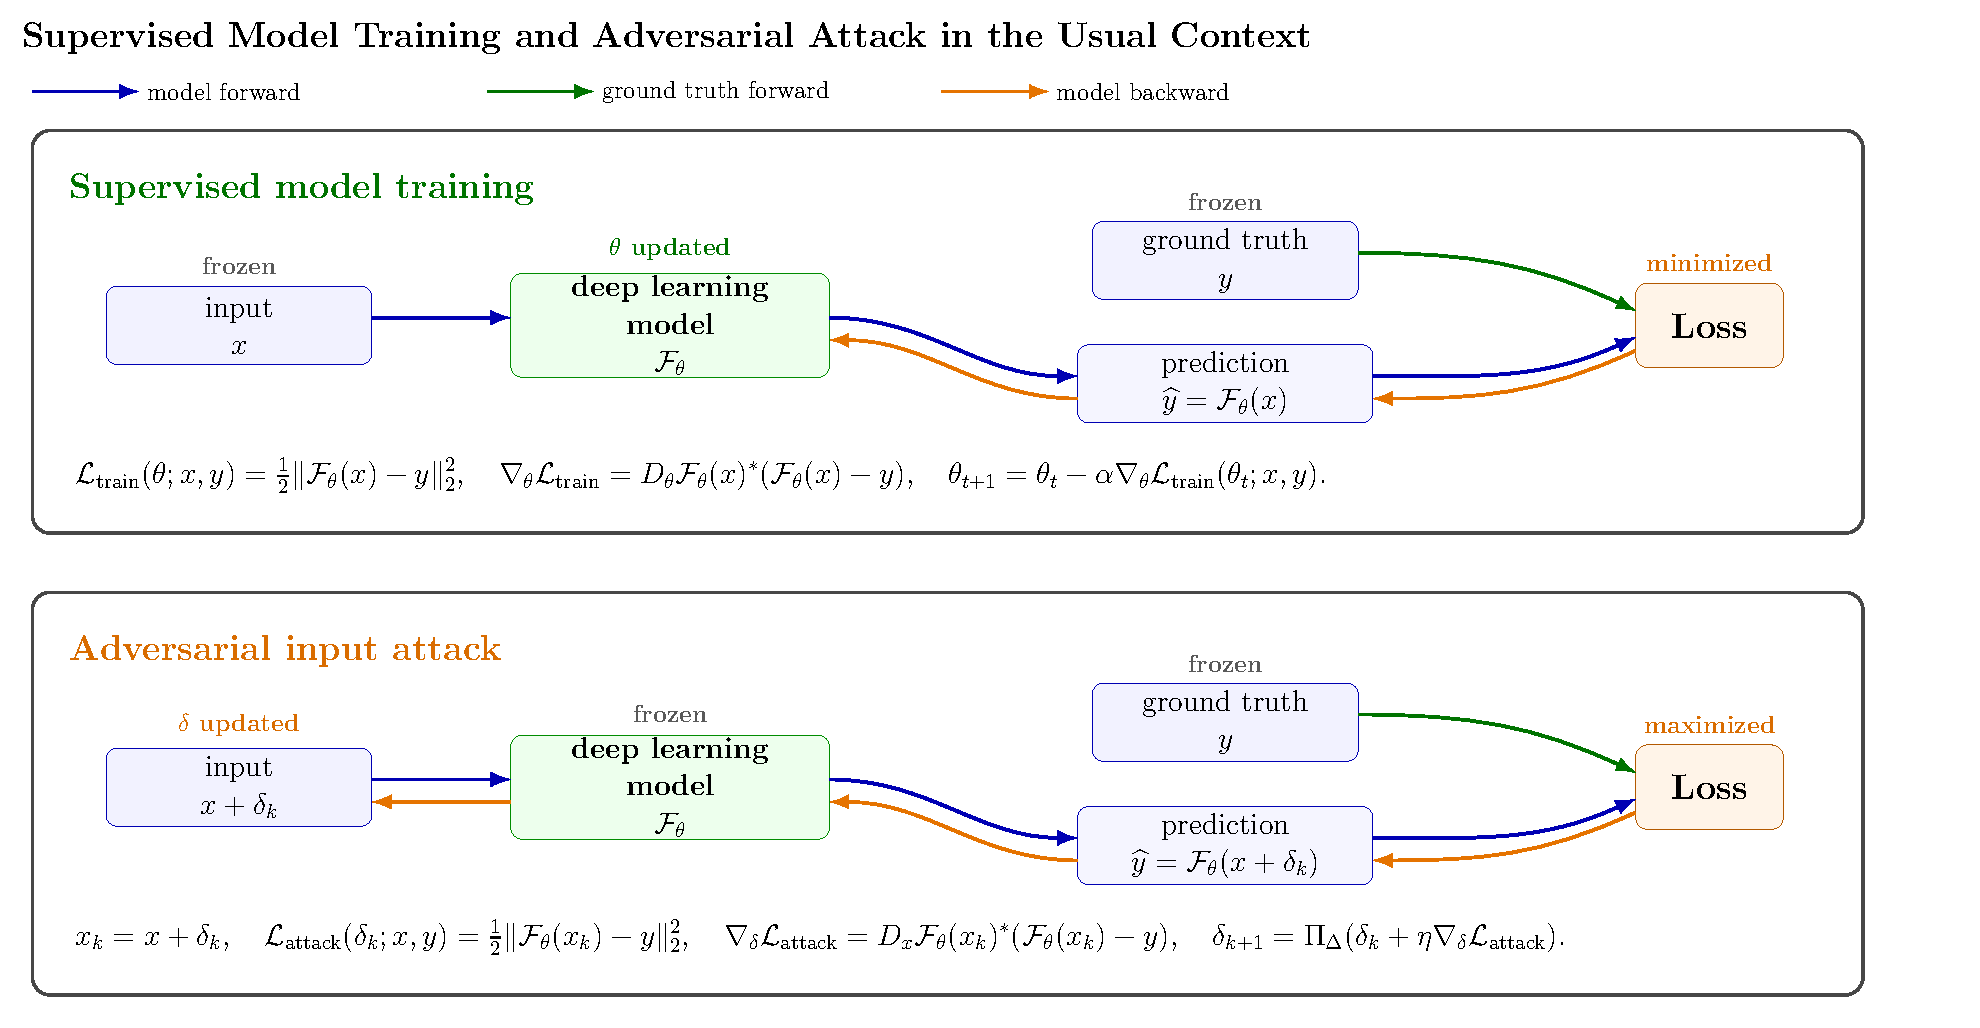
\includegraphics[width=0.94\textwidth]{figures/backpropagation_targets/compact/training_vs_attack_gradients.pdf}
  \caption{Training versus attack gradients. Training minimizes the loss by
  updating model parameters, whereas an adversarial attack maximizes the loss by
  updating the input perturbation.}
  \label{fig:training-vs-attack-gradients}
\end{figure}

\subsection*{PDE Operator Learning Attack and Training}

\begin{figure}[H]
  \centering
  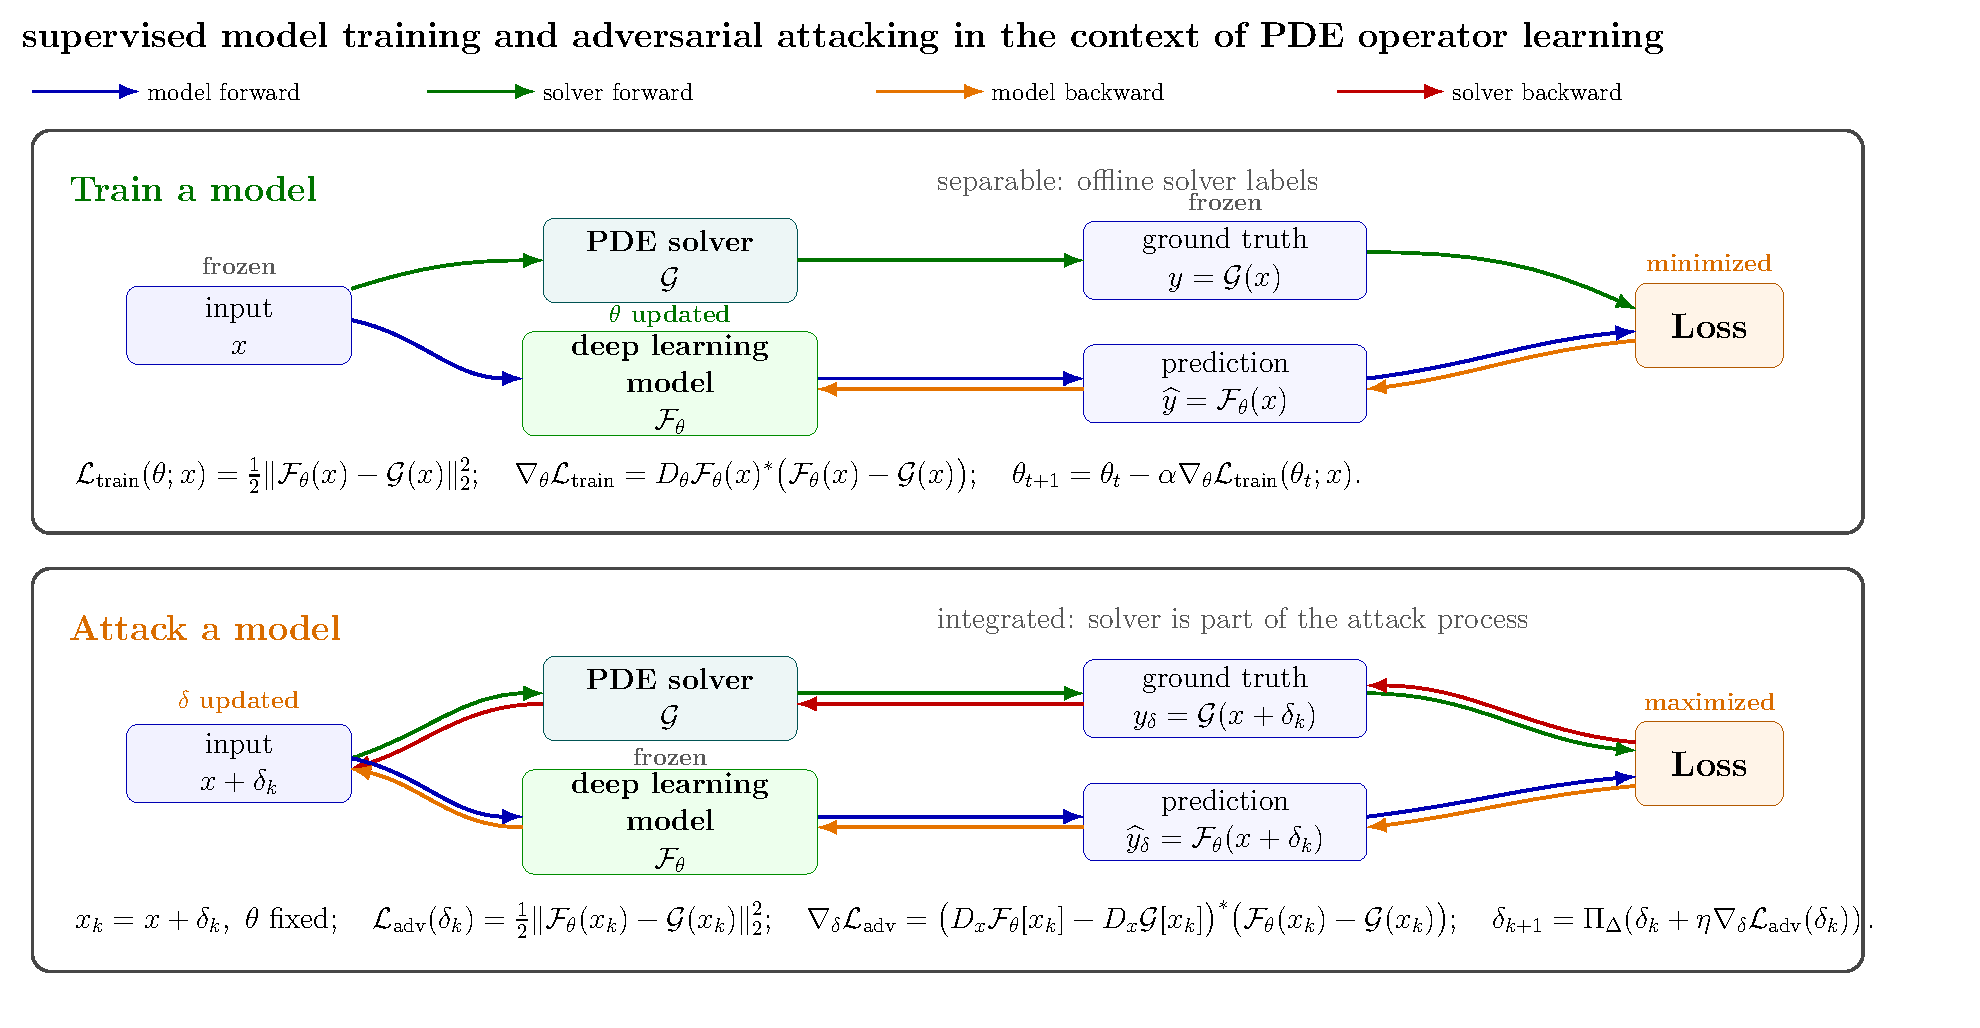
\includegraphics[width=0.94\textwidth]{figures/pde_solver_supervision/compact/pde_solver_training_attack.pdf}
  \caption{Supervised model training and adversarial attacking in PDE operator
  learning. The numerical solver maps the same input used by the model to the
  corresponding solver output, so it plays the role of a ground-truth oracle.}
  \label{fig:pde-solver-training-attack}
\end{figure}

\begin{figure}[H]
  \centering
  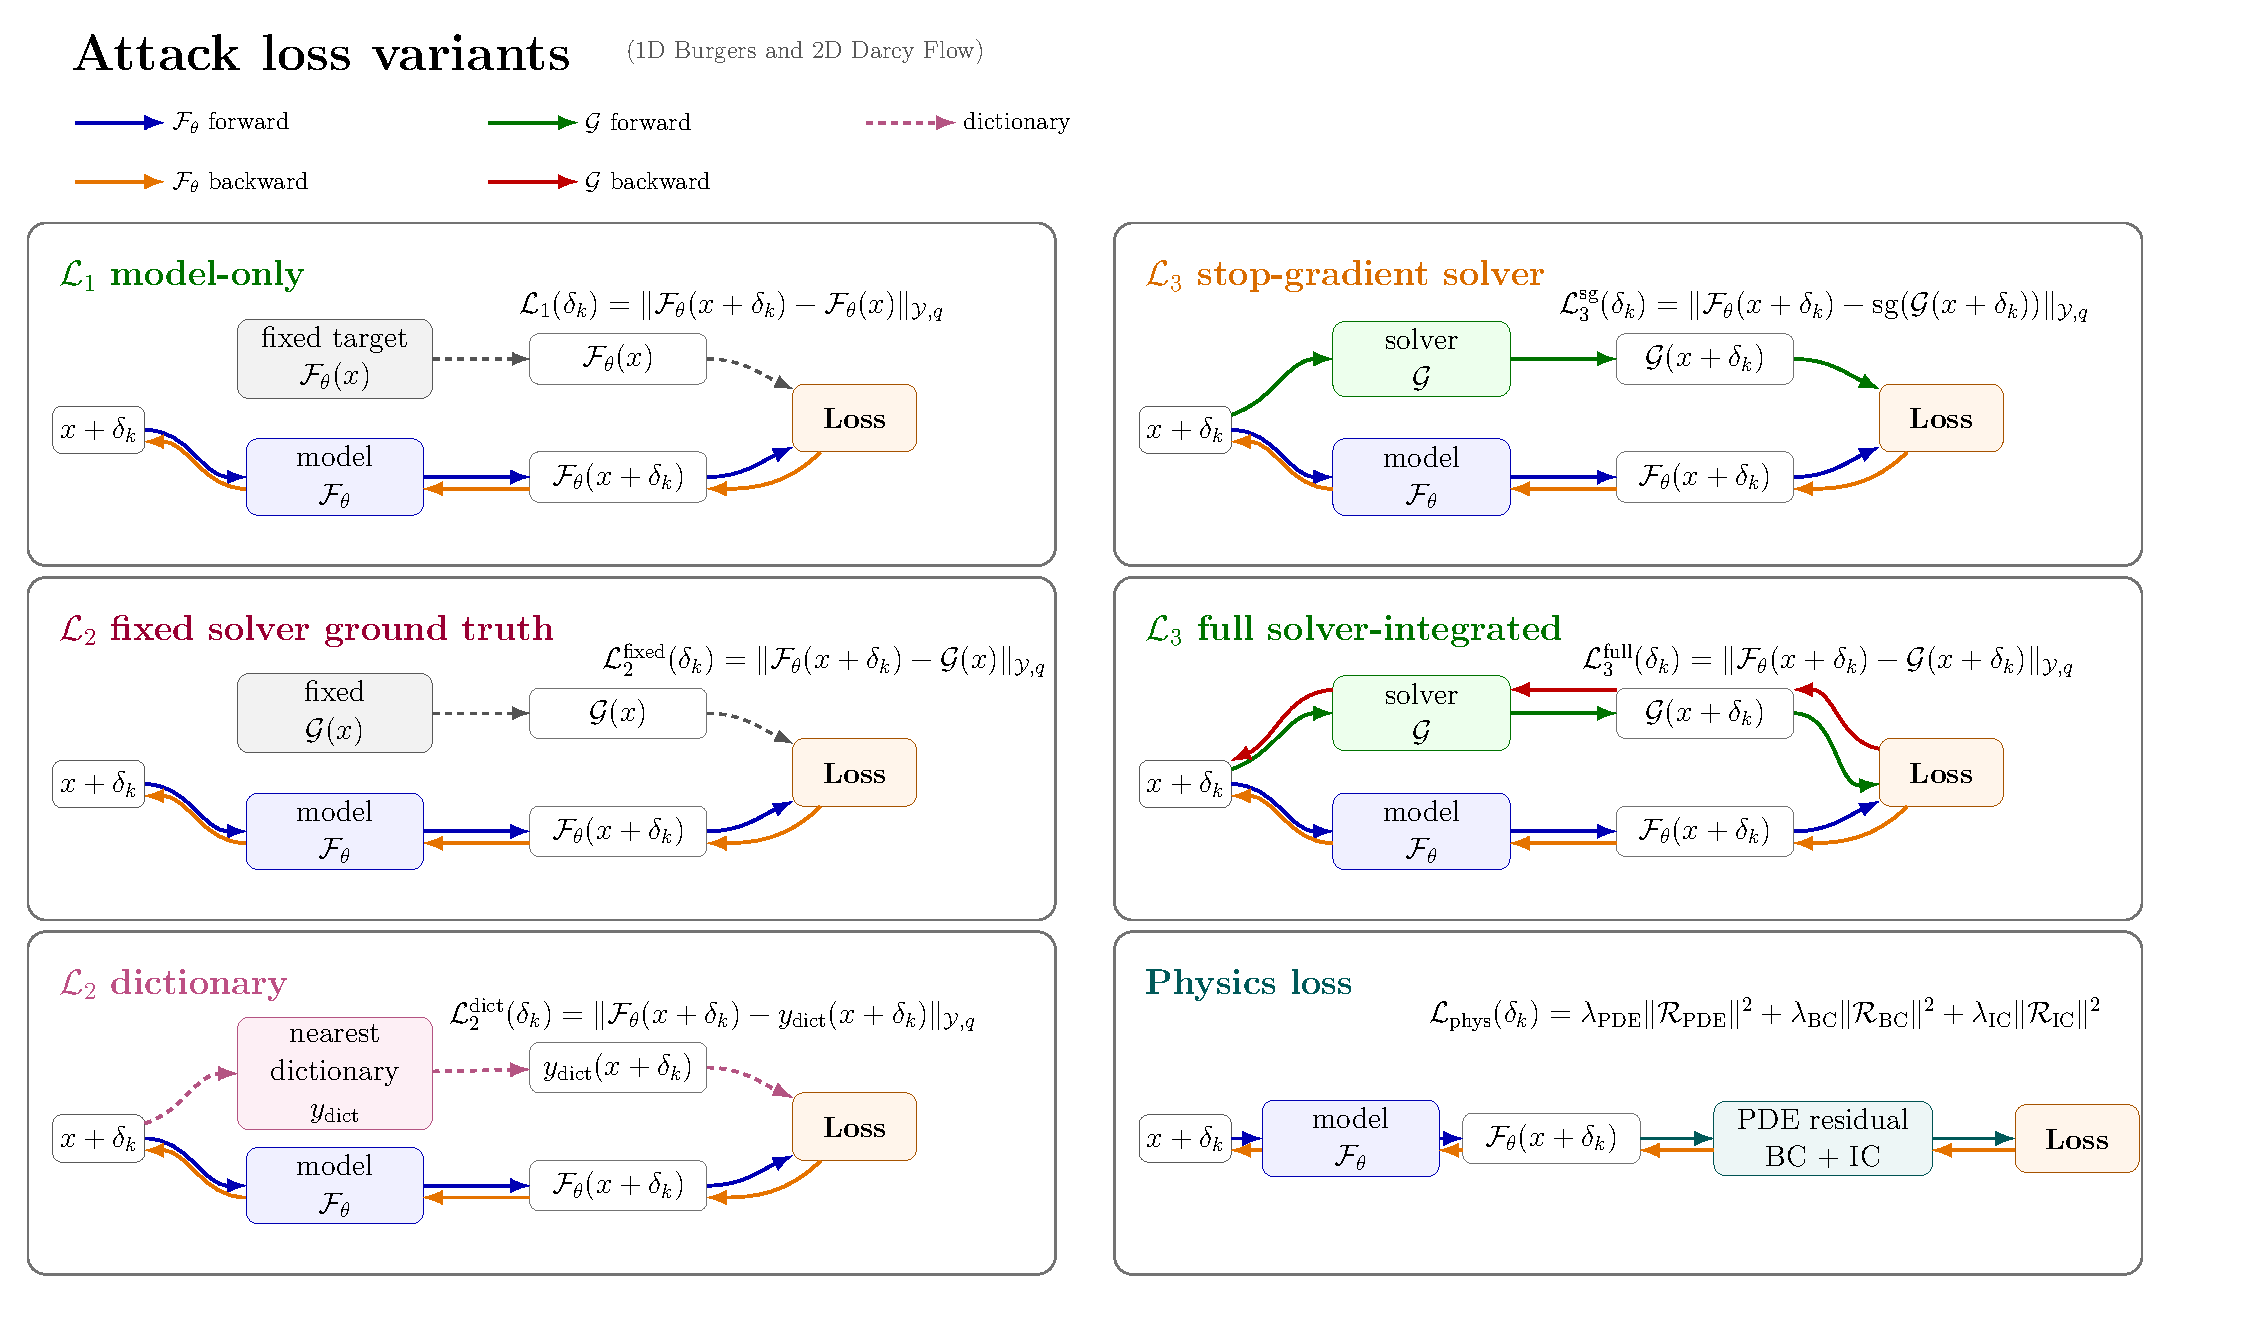
\includegraphics[width=0.94\textwidth]{figures/attack_loss_variants/non-compact/attack_loss_variants_twocol.pdf}
  \caption{Attack-loss variants arranged by solver integration. The variants
  range from model-only objectives, through fixed or dictionary targets, to
  stop-gradient and fully solver-integrated losses.}
  \label{fig:attack-loss-variants-twocol}
\end{figure}

\begin{figure}[H]
  \centering
  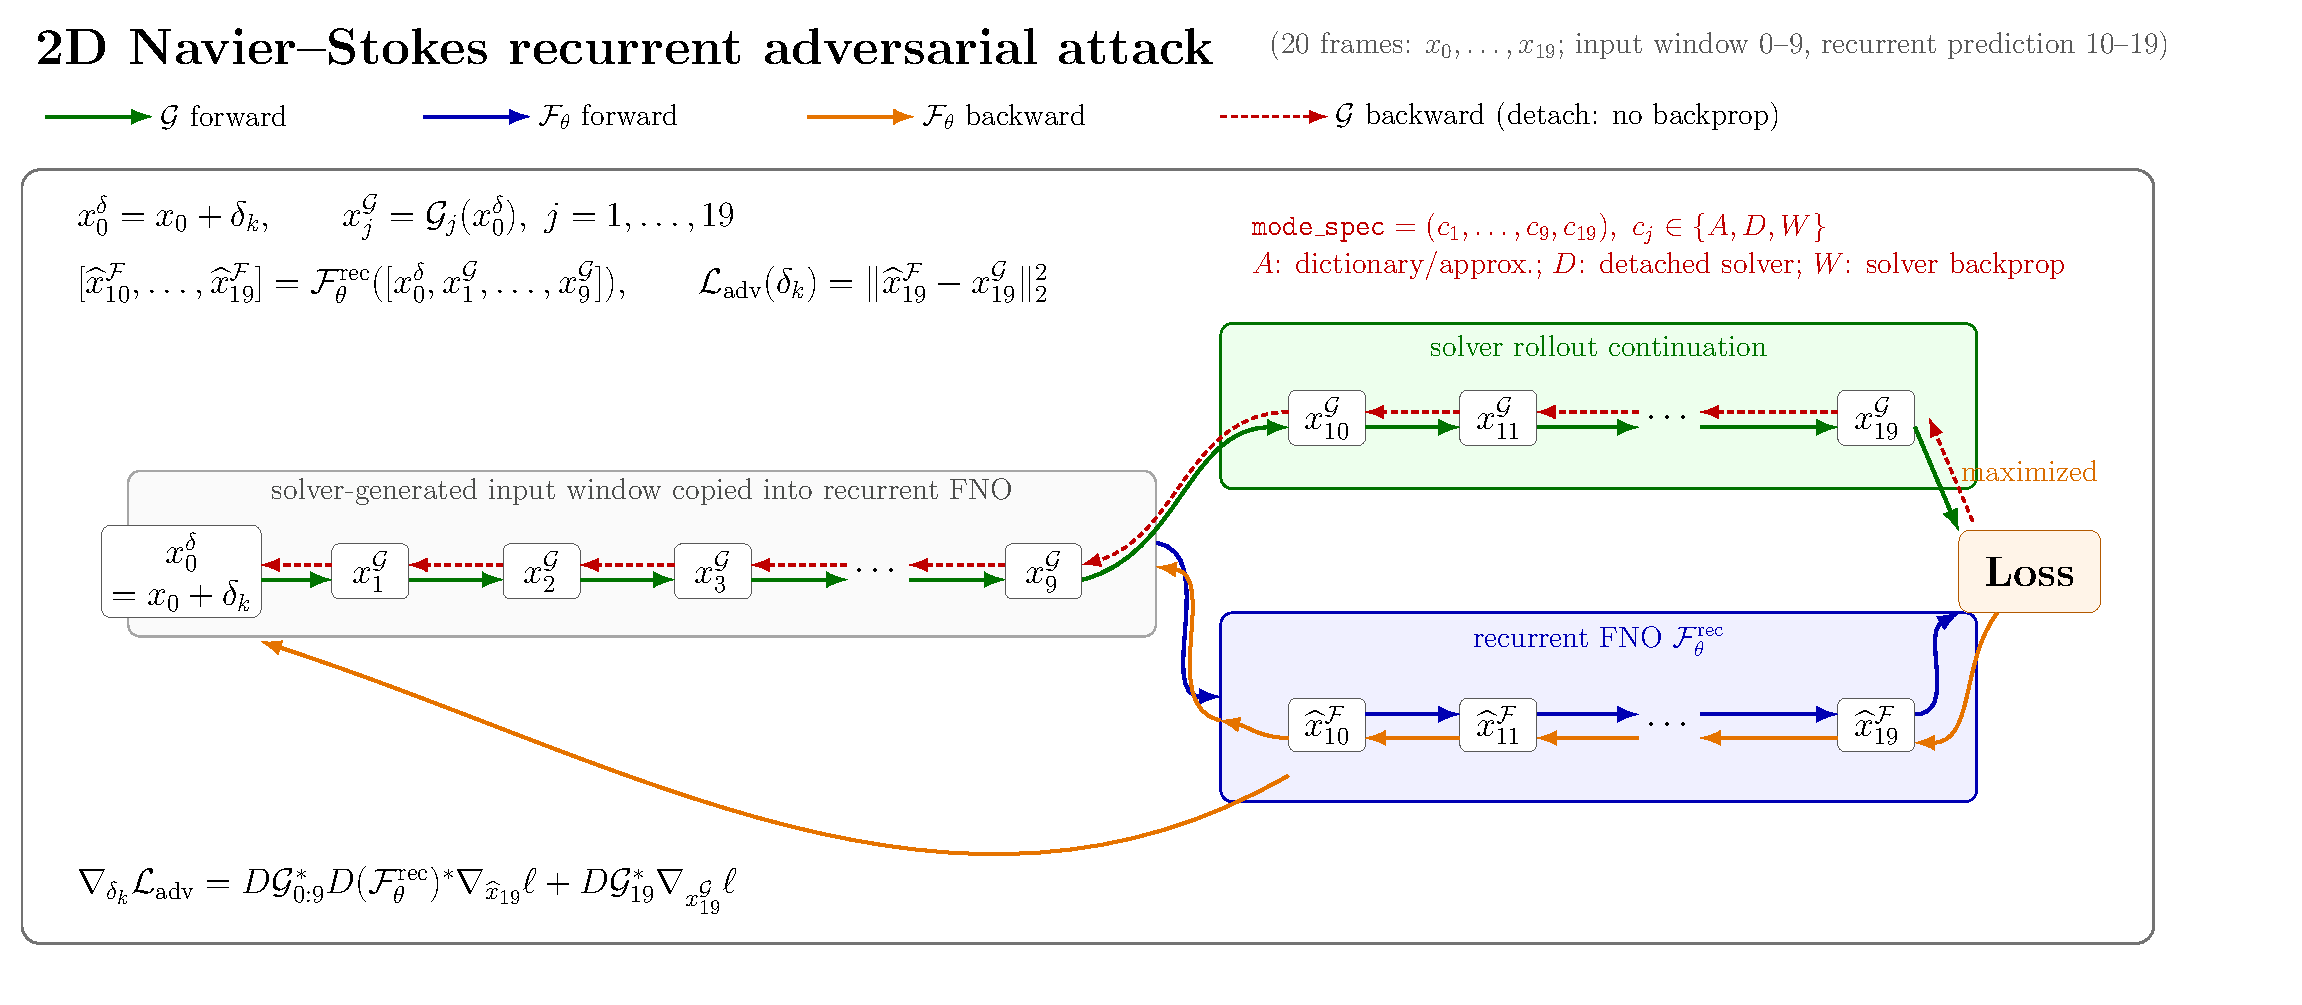
\includegraphics[width=0.94\textwidth]{figures/navier_stokes_recurrent/non-compact/ns_recurrent_adversarial_attack.pdf}
  \caption{Recurrent Navier--Stokes adversarial attack flow. The attack updates
  the initial vorticity input while the recurrent solver rollout supplies the
  target trajectory used in the loss.}
  \label{fig:ns-recurrent-adversarial-attack}
\end{figure}

\subsection*{Adversarial Training Pipelines}

\begin{figure}[H]
  \centering
  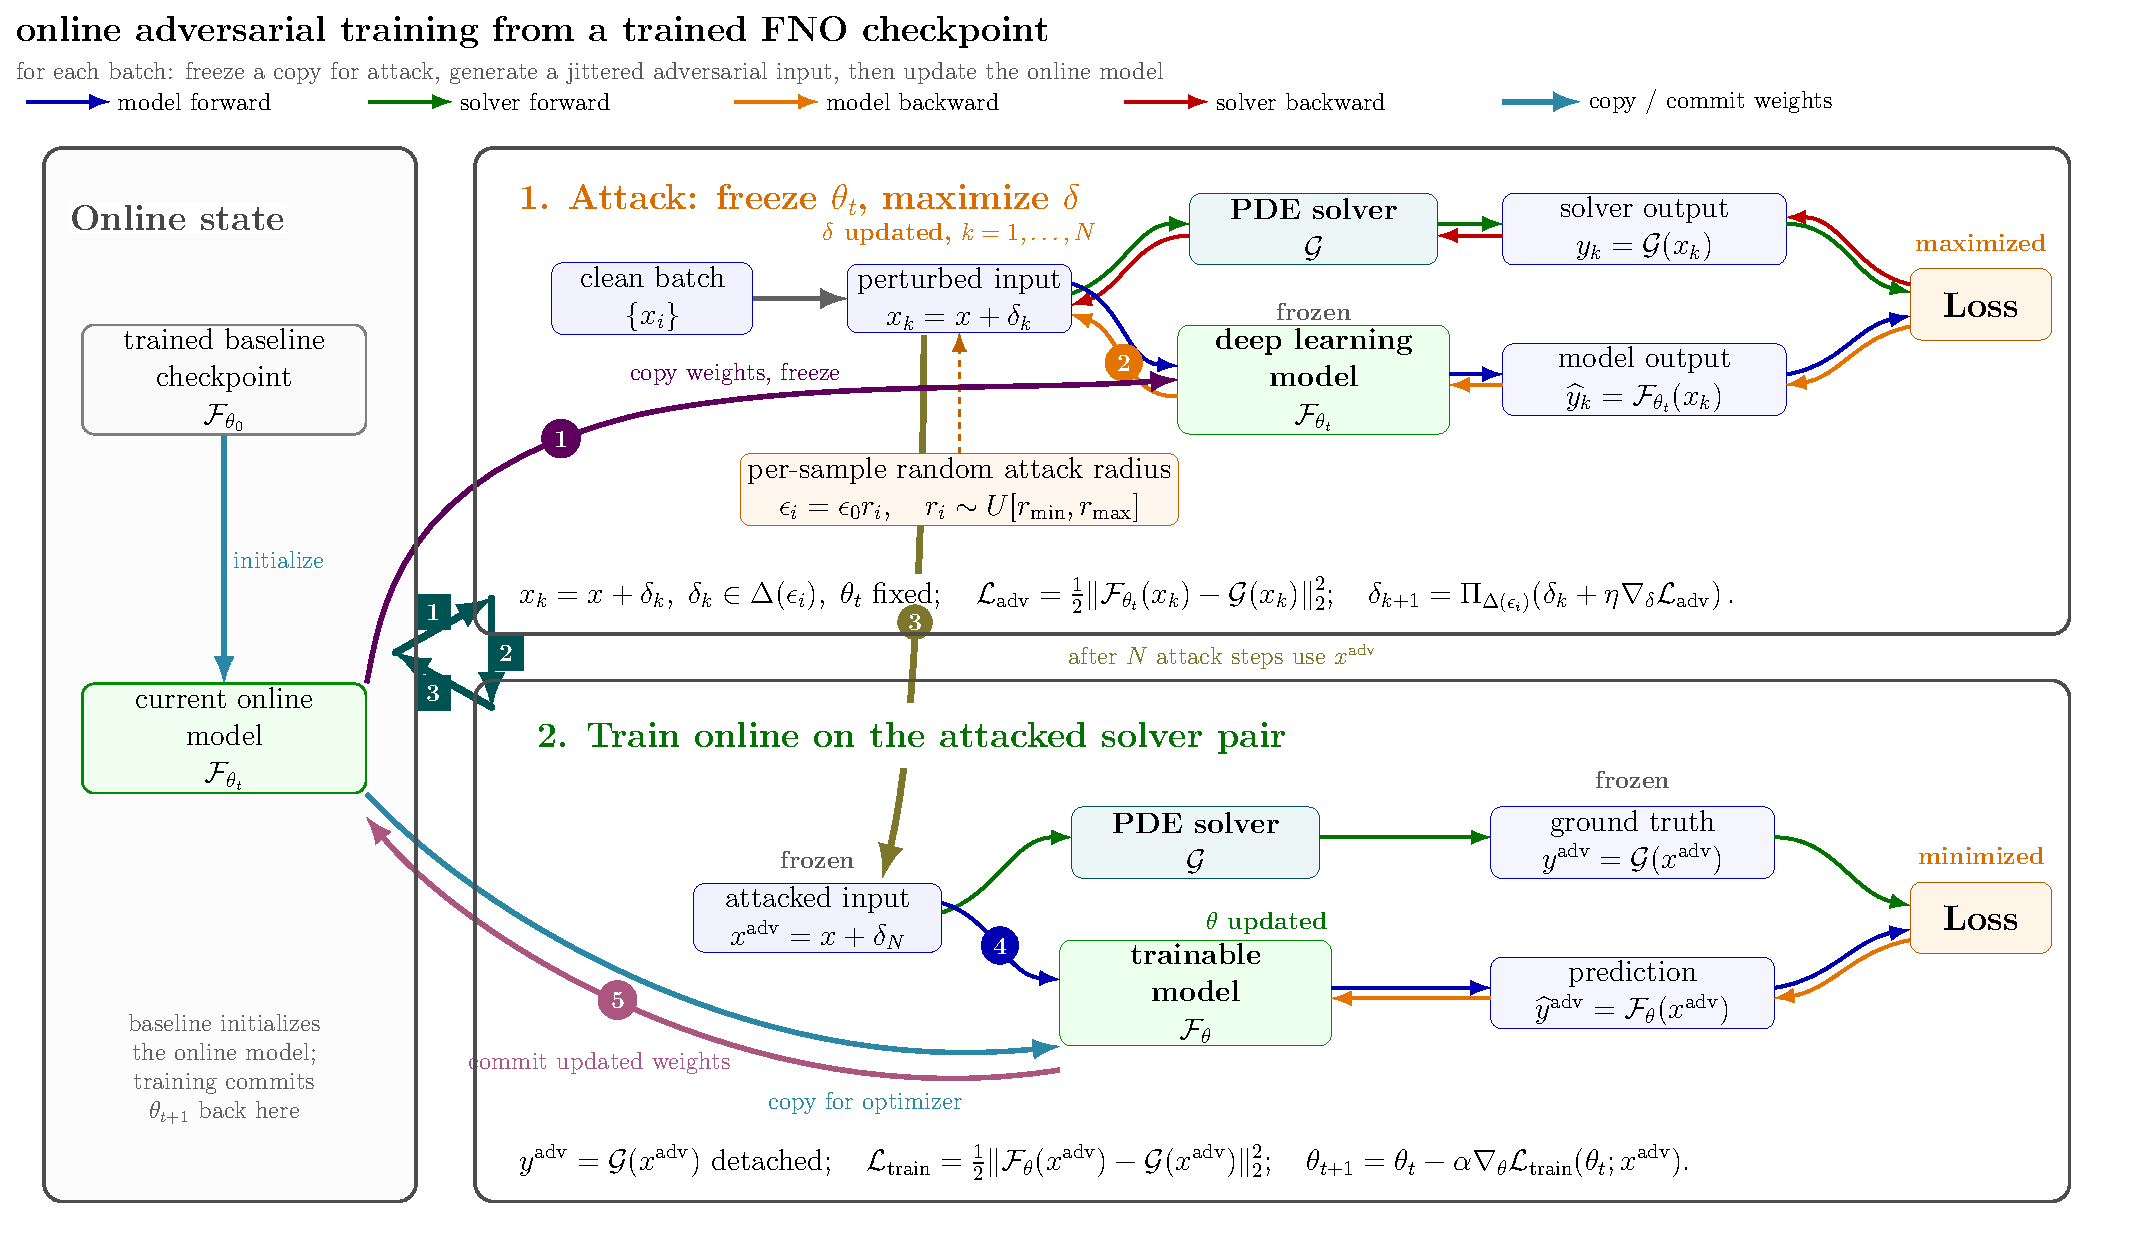
\includegraphics[width=0.92\textwidth]{figures/adversarial_training_pipeline/compact/adversarial_training_pipeline.pdf}
  \caption{Solver-integrated adversarial training pipeline. The current model
  is copied into the attack stage, adversarial inputs are generated, and the
  trainable model is updated on those attacked samples before becoming the next
  current model.}
  \label{fig:adversarial-training-pipeline}
\end{figure}

\begin{figure}[H]
  \centering
  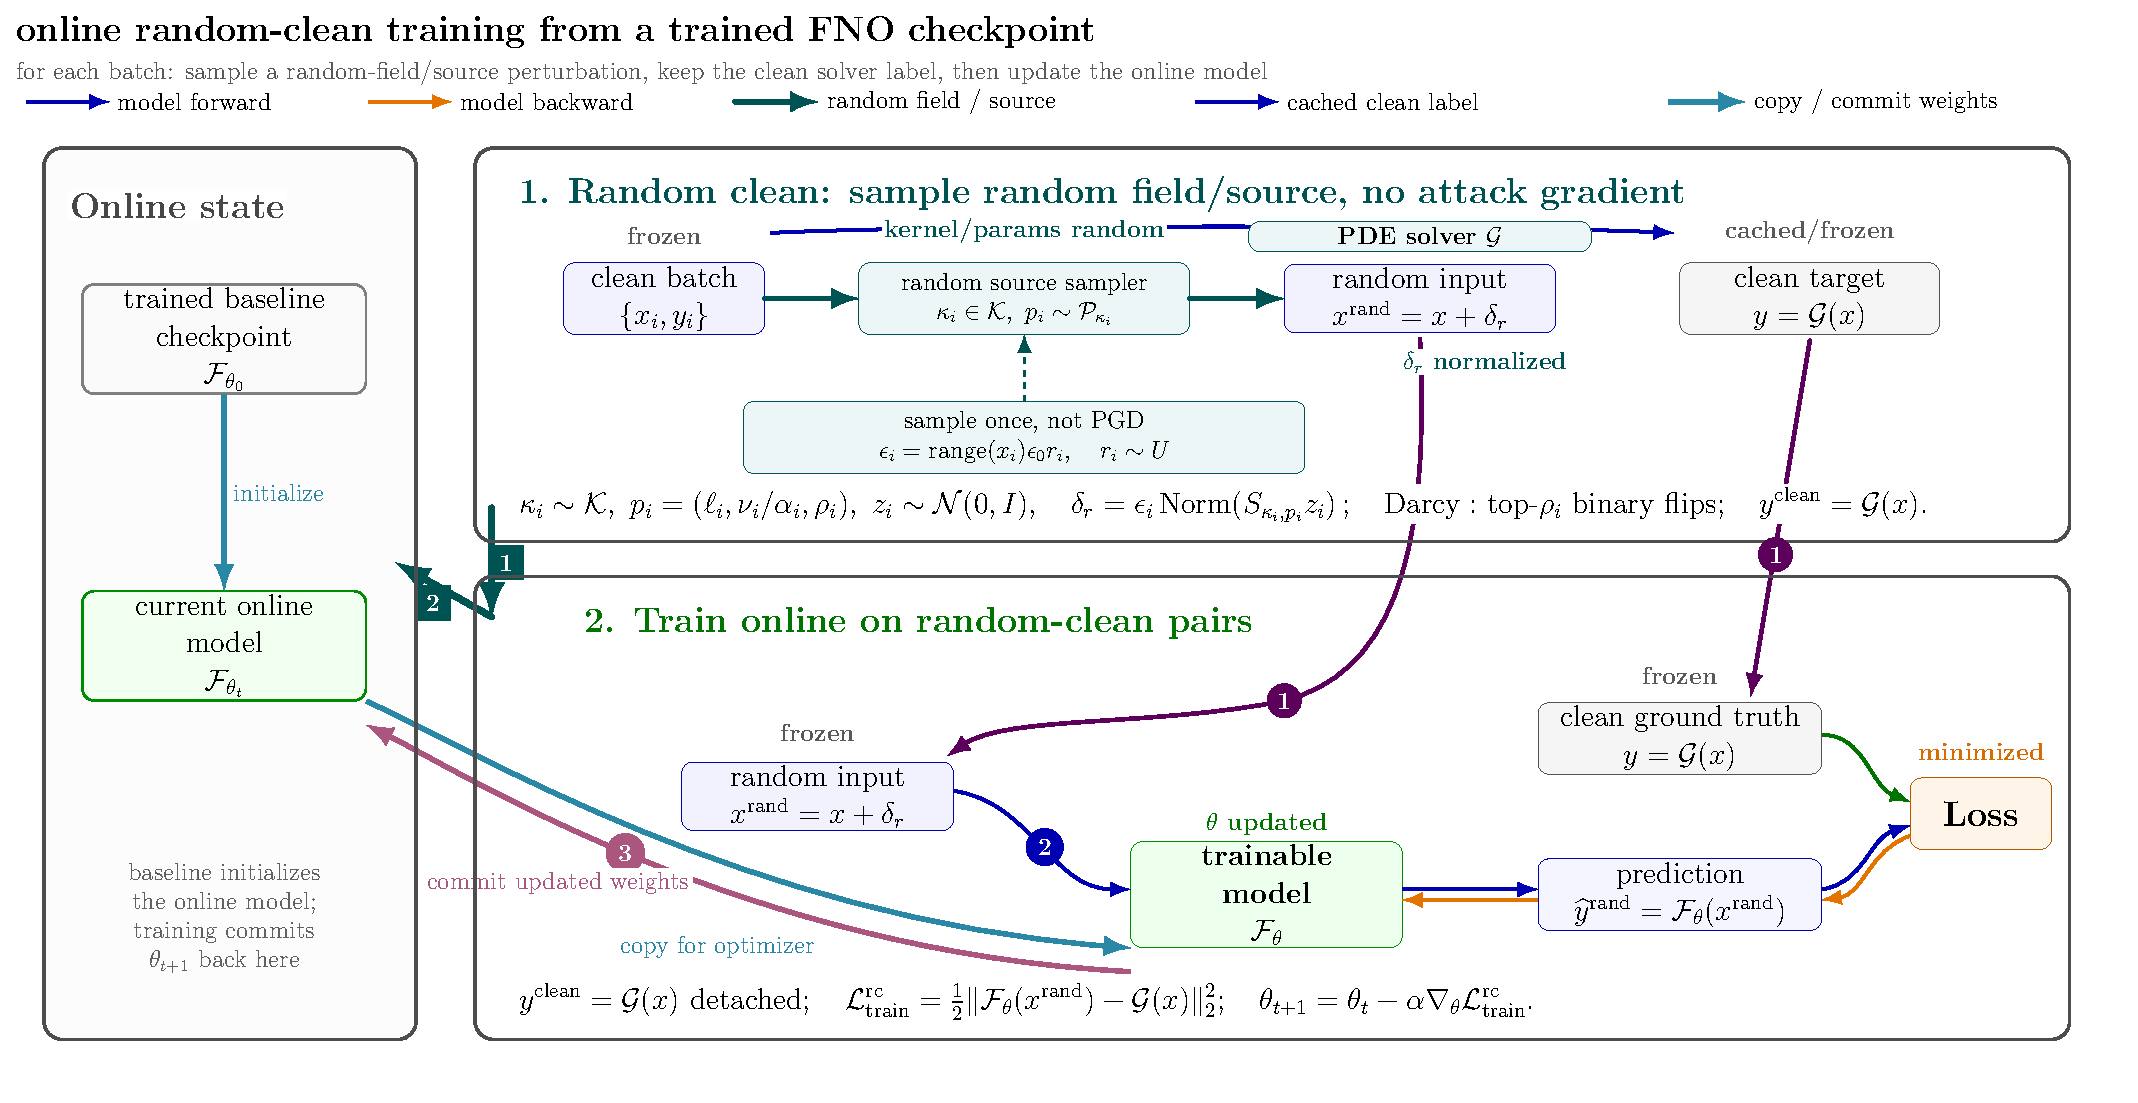
\includegraphics[width=0.92\textwidth]{figures/adversarial_training_pipeline/compact/random_clean_training_pipeline.pdf}
  \caption{Random-clean training pipeline. Perturbations are randomly sampled,
  and the perturbed inputs are trained against the original clean solver target.}
  \label{fig:random-clean-training-pipeline}
\end{figure}

\begin{figure}[H]
  \centering
  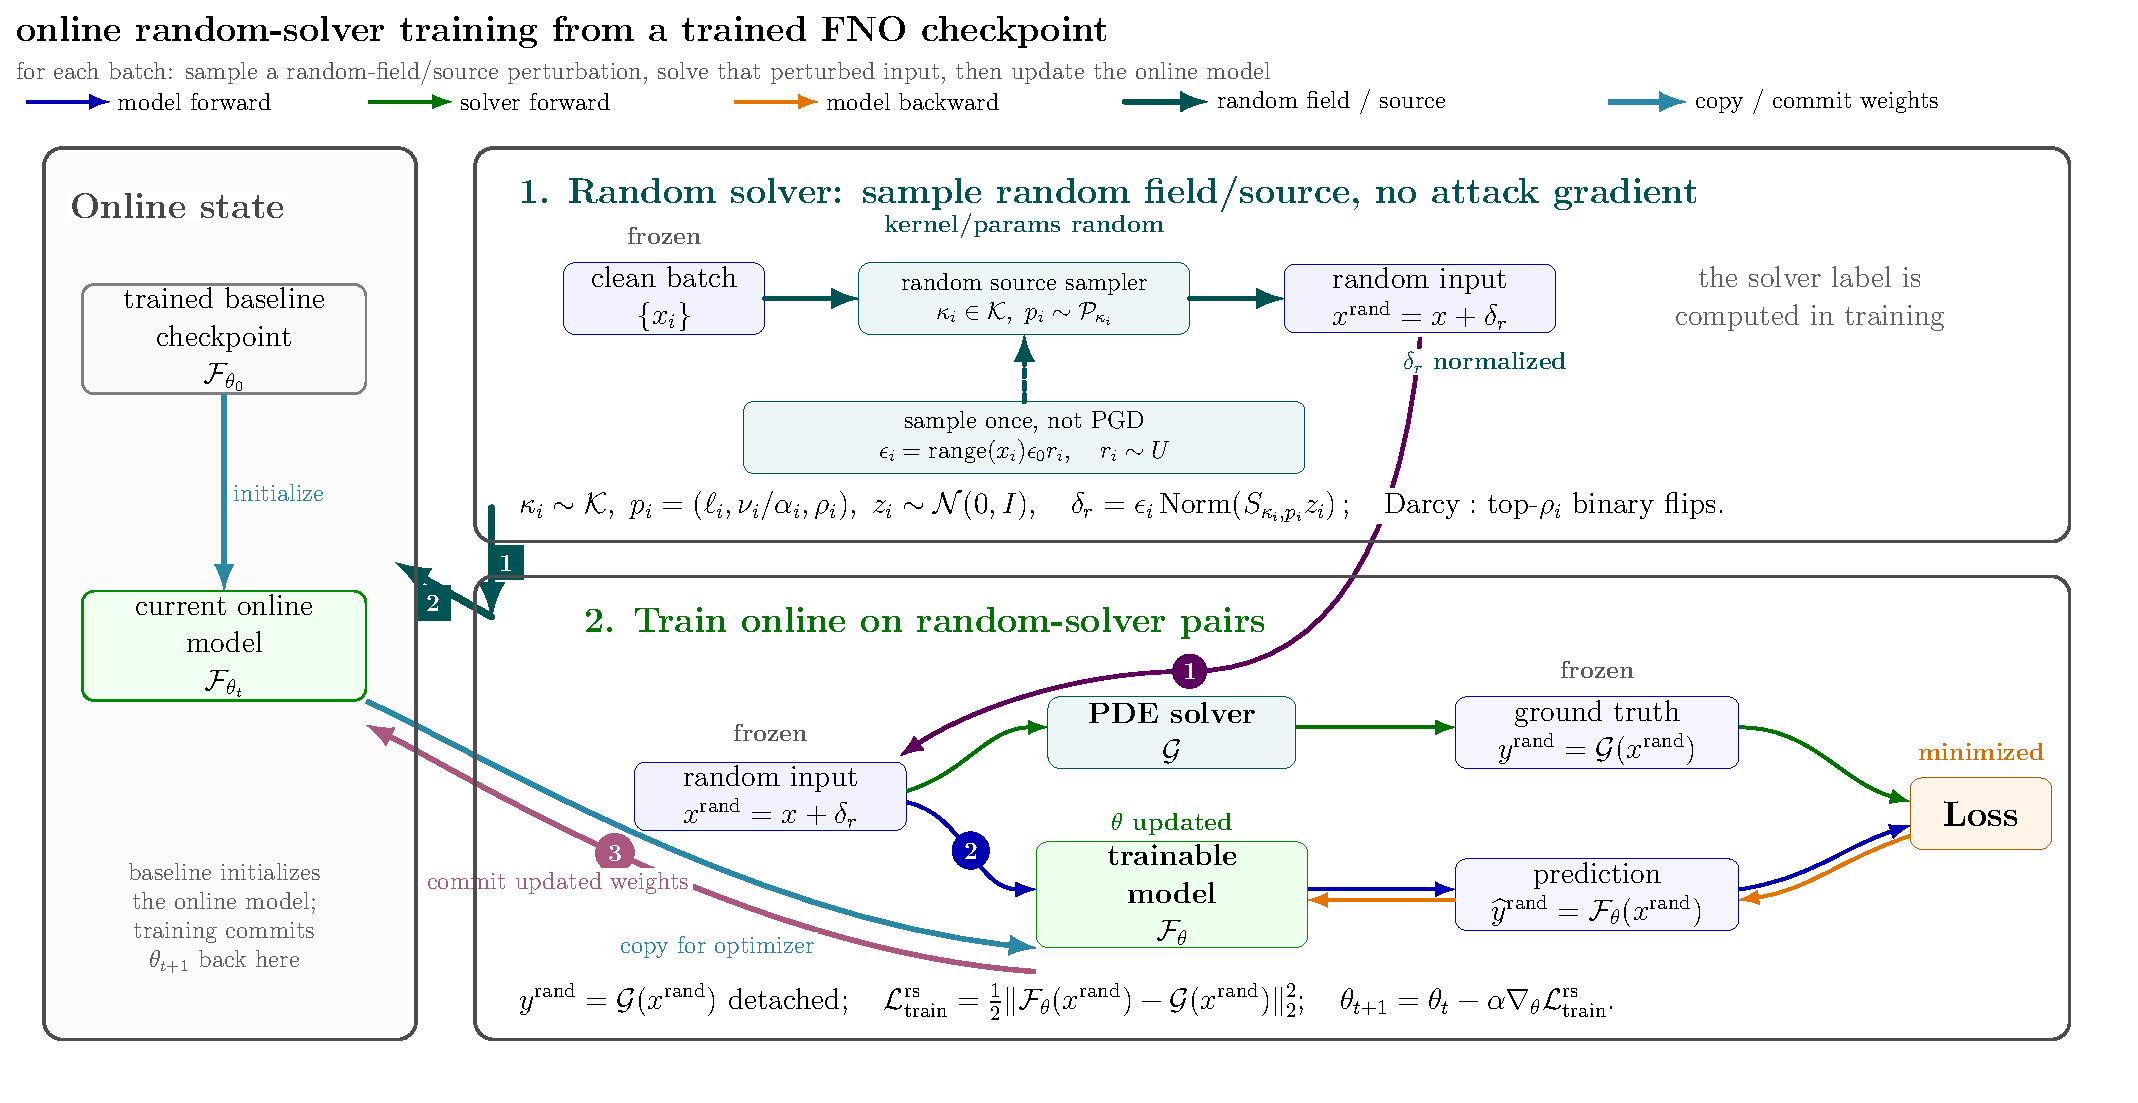
\includegraphics[width=0.92\textwidth]{figures/adversarial_training_pipeline/compact/random_solver_training_pipeline.pdf}
  \caption{Random-solver training pipeline. Perturbations are randomly sampled,
  and each perturbed input is relabeled by the solver output at that perturbed
  input.}
  \label{fig:random-solver-training-pipeline}
\end{figure}

\subsection*{PGD visualization}

\begin{figure}[H]
  \centering
  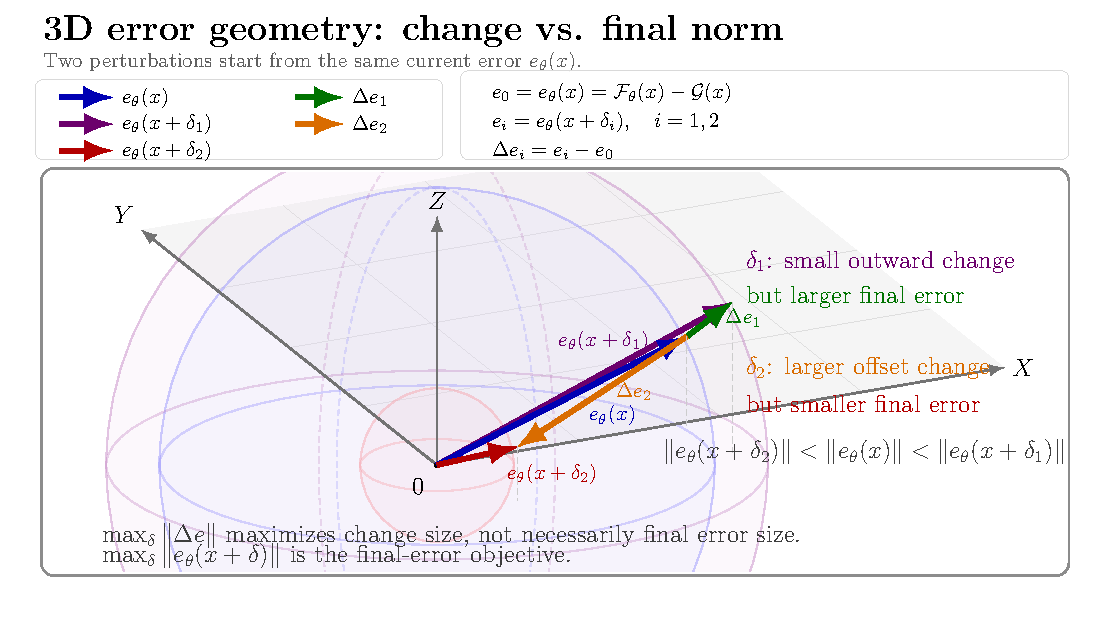
\includegraphics[width=0.86\textwidth]{figures/error_vector_geometry/compact/error_difference_vs_final_norm.pdf}
  \caption{Error-vector geometry for adversarial loss increase. The figure
  contrasts final error norm growth with the error-difference direction used by
  local Jacobian-error diagnostics.}
  \label{fig:error-difference-vs-final-norm}
\end{figure}

\begin{figure}[H]
  \centering
  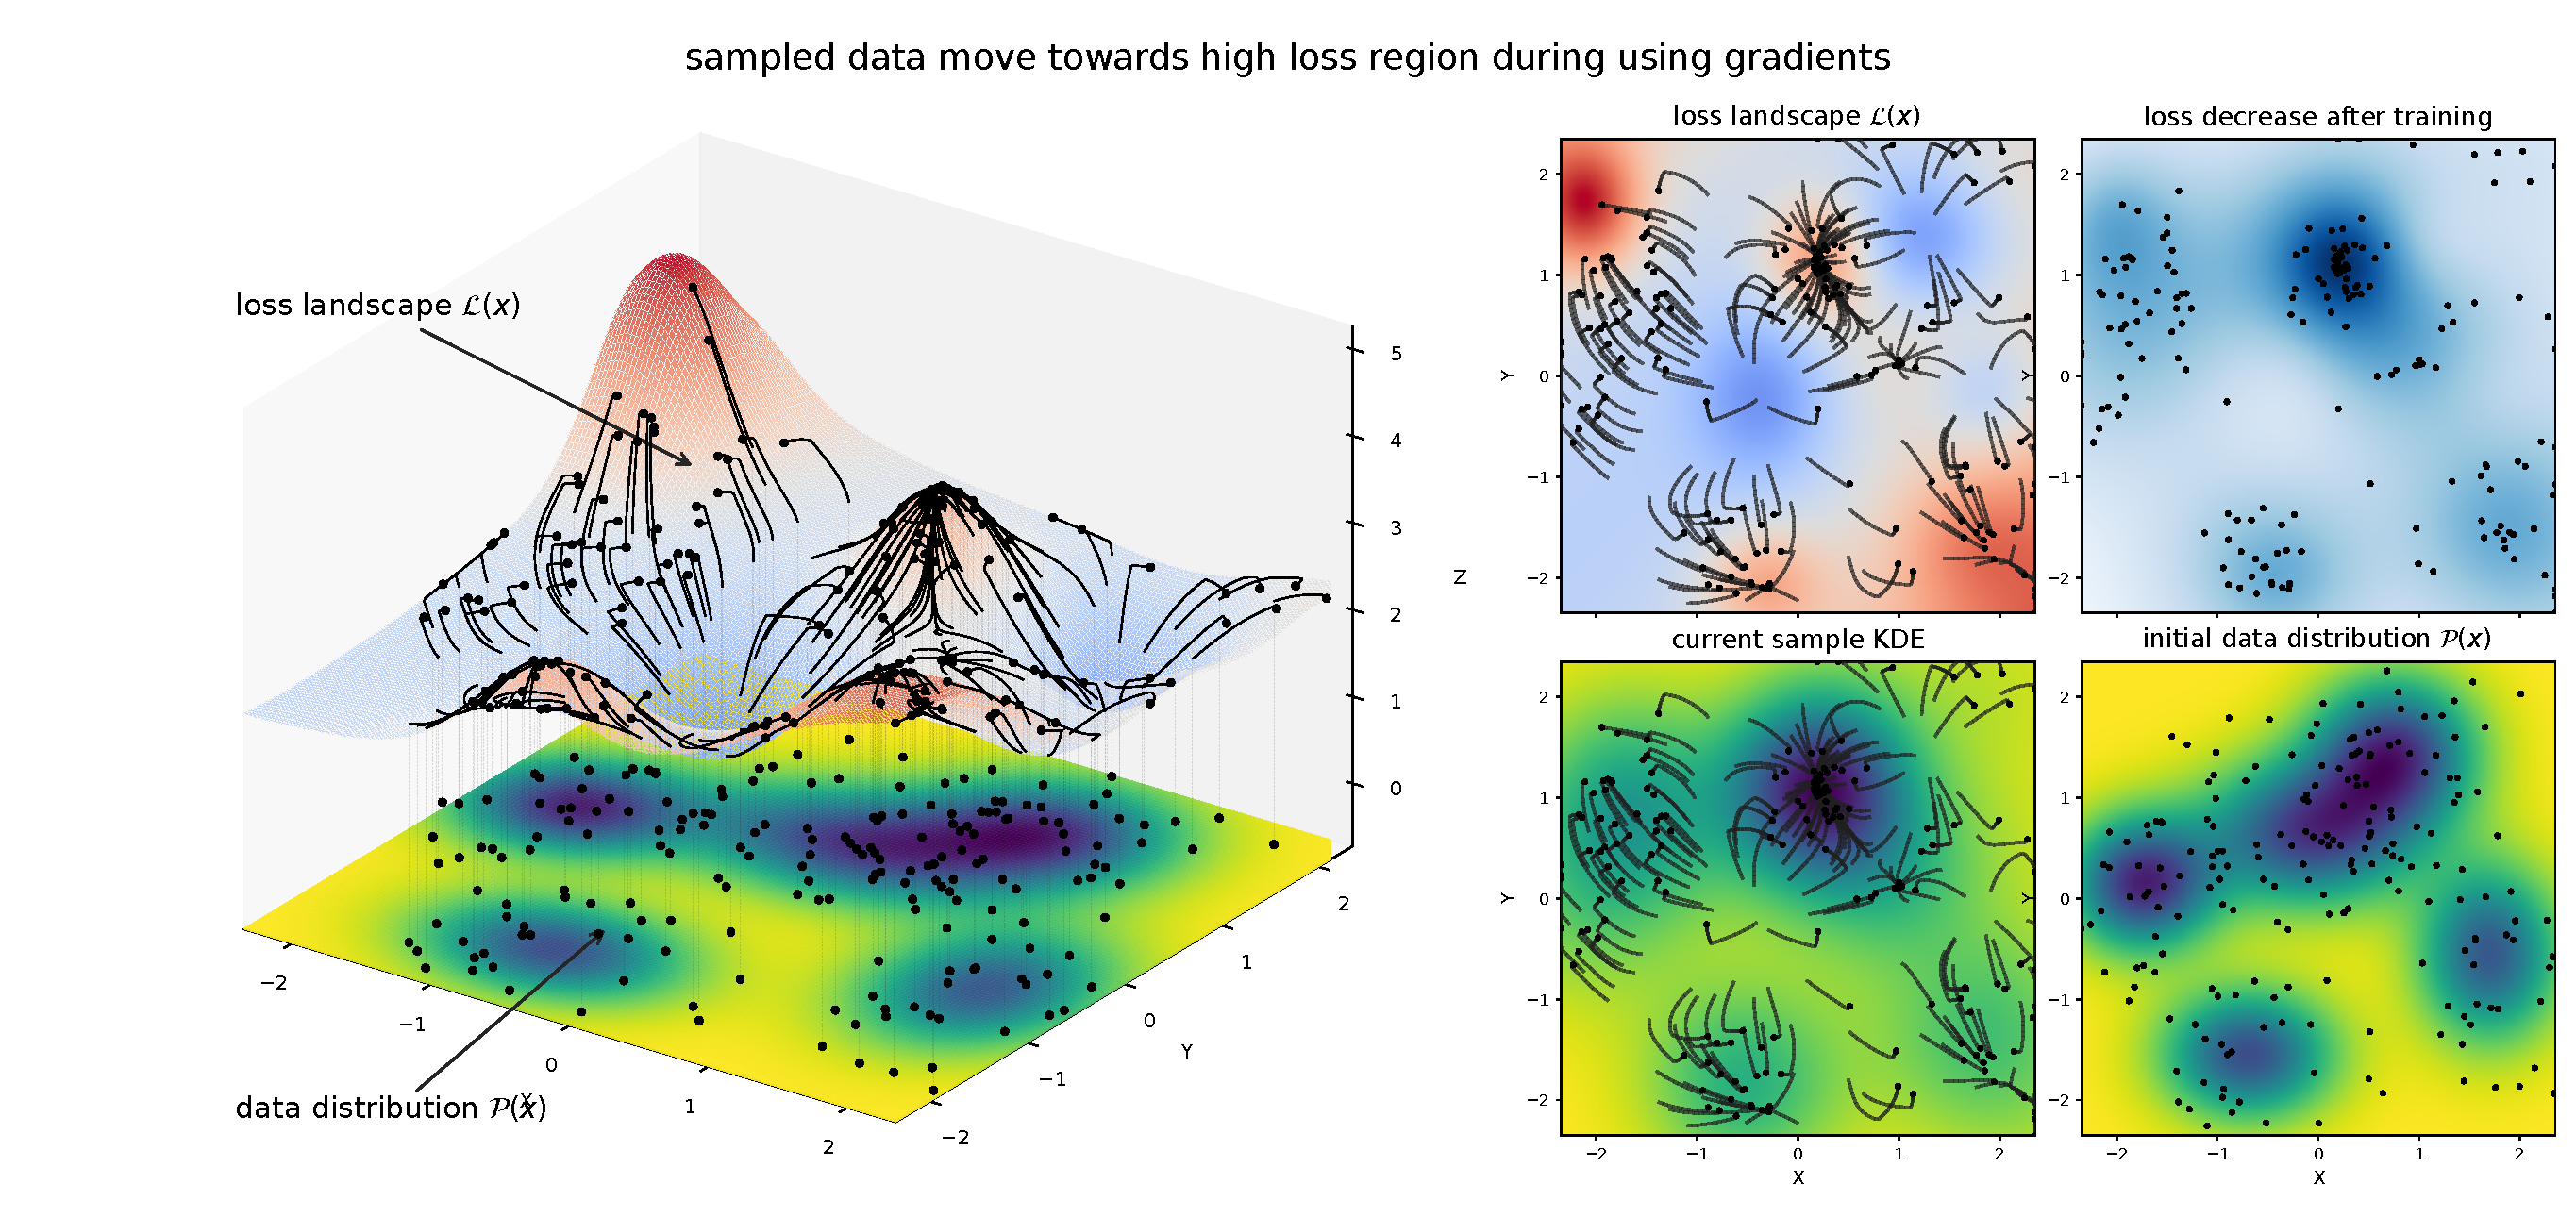
\includegraphics[width=0.98\textwidth]{figures/loss_landscape/non-compact/loss_landscape.pdf}
  \caption{Low-dimensional PGD visualization of high-dimensional
  function-space sampling. Samples drawn from the dataset distribution
  \(\mathcal{P}(x)\) move along gradients of the loss landscape
  \(\mathcal{L}(x)\), blending data density with loss information and
  concentrating samples in high-loss regions.}
  \label{fig:loss-landscape-pgd-visualization}
\end{figure}

\clearpage

\endgroup

\begingroup
\captionsetup[figure]{skip=2pt}
\setlength{\intextsep}{5pt}
\setlength{\textfloatsep}{5pt}
\setlength{\floatsep}{5pt}
\newcommand{\appendixattackfig}[3]{%
\begin{figure}[H]
  \centering
  \includegraphics[width=0.96\textwidth,height=0.82\textheight,keepaspectratio]{#1}
  \caption{#2}
  \label{#3}
\end{figure}
}
\newcommand{\appendixattackfigcompact}[3]{%
\begin{figure}[H]
  \centering
  \includegraphics[width=\textwidth,height=0.455\textheight,keepaspectratio]{#1}
  \caption{#2}
  \label{#3}
\end{figure}
}
\newcommand{\appendixattackfighalf}[3]{%
\begin{figure}[H]
  \centering
  \includegraphics[width=0.98\textwidth,height=0.405\textheight,keepaspectratio]{#1}
  \caption{#2}
  \label{#3}
\end{figure}
}
\newcommand{\appendixattackfigwidehalf}[3]{%
\begin{figure}[H]
  \centering
  \captionsetup{skip=1pt}
  \includegraphics[width=\textwidth,height=0.405\textheight,keepaspectratio]{#1}
  \caption{#2}
  \label{#3}
\end{figure}
}
\newcommand{\appendixattackfigwidehalflarge}[3]{%
\begin{figure}[H]
  \centering
  \captionsetup{skip=1pt}
  \includegraphics[width=\textwidth,height=0.405\textheight,keepaspectratio]{#1}
  \caption{#2}
  \label{#3}
\end{figure}
}
\newcommand{\appendixattackfigdarcygenhalf}[3]{%
\begin{figure}[H]
  \centering
  \captionsetup{skip=1pt}
  \includegraphics[width=\textwidth,height=0.455\textheight,keepaspectratio]{#1}
  \caption{#2}
  \label{#3}
\end{figure}
}
\newcommand{\appendixattackfigportraitwide}[3]{%
\begin{figure}[H]
  \centering
  \includegraphics[width=0.99\textwidth,height=0.74\textheight,keepaspectratio]{#1}
  \caption{#2}
  \label{#3}
\end{figure}
}
\newcommand{\appendixattackfigportraitwidelarge}[3]{%
\begin{figure}[H]
  \centering
  \captionsetup{skip=1pt}
  \includegraphics[width=0.99\textwidth,height=0.82\textheight,keepaspectratio]{#1}
  \caption{#2}
  \label{#3}
\end{figure}
}
\newcommand{\appendixtrainingfigportraitwide}[3]{%
\begin{figure}[H]
  \centering
  \captionsetup{skip=1pt}
  \includegraphics[width=0.99\textwidth,height=0.80\textheight,keepaspectratio]{#1}
  \caption{#2}
  \label{#3}
\end{figure}
}
\newcommand{\appendixattackfigstacked}[3]{%
\begin{figure}[H]
  \centering
  \captionsetup{skip=1pt}
  \includegraphics[width=0.99\textwidth,height=0.38\textheight,keepaspectratio]{#1}
  \caption{#2}
  \label{#3}
\end{figure}
}
\newcommand{\appendixattackfigfullportrait}[3]{%
\begin{figure}[H]
  \centering
  \captionsetup{skip=1pt}
  \includegraphics[width=\textwidth,height=0.88\textheight,keepaspectratio]{#1}
  \caption{#2}
  \label{#3}
\end{figure}
}
\newcommand{\appendixattackfigfullwidth}[3]{%
\begin{figure}[H]
  \centering
  \captionsetup{skip=1pt}
  \includegraphics[width=\textwidth,height=0.88\textheight,keepaspectratio]{#1}
  \caption{#2}
  \label{#3}
\end{figure}
}
\newcommand{\appendixdomainheading}[1]{%
  \refstepcounter{appendixdomain}%
  \par\medskip
  \noindent{\normalsize\bfseries \theappendixdomain\ #1}\par\smallskip
}

% Do not force a new page here; this appendix should follow the diagram
% appendix without an extra page break.
\appendixsection{Solver-Integrated Attack and Training Figure Appendix}{app:si-attack-training-figures}

\appendixsubsection{Solver-Integrated Adversarial Attack}

\appendixdomainheading{Burgers}

\noindent\textbf{Burgers: FNO final prediction and perturbation fields.}

\clearpage

\appendixattackfigcompact
  {figures/adversarial_attack_appendix/attack/burgers/fno/final_prediction_delta/slide13_burgers_fno_l2_pgd_loss_variants_final_frame.png}
  {Burgers FNO $L_2$ PGD attack variants, including final perturbed inputs,
  model/solver predictions, residuals, and loss curves. Only optimizing Loss 3
  maximizes the true model--solver loss; optimizing the other losses often does
  not maximize the true discrepancy between the solver and the model.}
  {fig:app-g-burgers-fno-l2-final}

\appendixattackfigcompact
  {figures/adversarial_attack_appendix/attack/burgers/fno/final_prediction_delta/slide15_burgers_fno_linf_pgd_loss_variants_final_frame.png}
  {Burgers FNO $L_\infty$ PGD attack variants, including final perturbed
  inputs, model/solver predictions, residuals, and loss curves.}
  {fig:app-g-burgers-fno-linf-final}

\clearpage

\noindent\textbf{Burgers: FNO loss progression.}

\appendixattackfig
  {figures/adversarial_attack_appendix/attack/burgers/fno/loss_progression/slide18_burgers_fno_l2_loss_progression_mean_std.png}
  {Burgers FNO $L_2$ attack loss progression with mean and standard-deviation
  bands across PGD steps.}
  {fig:app-g-burgers-fno-l2-loss}

\appendixattackfig
  {figures/adversarial_attack_appendix/attack/burgers/fno/loss_progression/burgers_fno_linf_eps0p3_alpha0p03_loss_progression_mean_std_linear.png}
  {Burgers FNO $L_\infty$ attack loss progression with mean and
  standard-deviation bands at $\varepsilon=0.3$ and $\alpha=0.03$.}
  {fig:app-g-burgers-fno-linf-eps03-loss}

\FloatBarrier
\noindent\textbf{Burgers: DeepONet final prediction and perturbation fields.}


\appendixattackfig
  {figures/adversarial_attack_appendix/attack/burgers/deeponet/final_prediction_delta/slide19_burgers_final_state_comparison_steepest_add.png}
  {Burgers final-state comparison for the Steepest Add optimizer, showing the
  clean baseline, attacked inputs, final predictions, solver outputs, residuals,
  and loss-specific panels. In Burgers, the Delta perturbations optimized by
  loss 3 are often visibly higher-frequency.}
  {fig:app-g-burgers-steepest-add-final}

\appendixattackfigcompact
  {figures/adversarial_attack_appendix/attack/burgers/deeponet/final_prediction_delta/slide20_burgers_deeponet_l2_pgd_loss_variants_final_frame.png}
  {Burgers DeepONet $L_2$ PGD attack variants with final prediction and
  perturbation comparisons. Only optimizing Loss 3 maximizes the true
  model--solver loss; optimizing the other losses often does not maximize the
  true discrepancy between the solver and the model.}
  {fig:app-g-burgers-deeponet-l2-final}

\appendixattackfigcompact
  {figures/adversarial_attack_appendix/attack/burgers/deeponet/final_prediction_delta/slide22_burgers_deeponet_linf_pgd_loss_variants_final_frame.png}
  {Burgers DeepONet $L_\infty$ PGD attack variants with final prediction and
  perturbation comparisons.}
  {fig:app-g-burgers-deeponet-linf-final}

\noindent\textbf{Burgers: DeepONet loss progression.}

\appendixattackfig
  {figures/adversarial_attack_appendix/attack/burgers/deeponet/loss_progression/slide17_burgers_deeponet_l2_loss_progression_mean_std.png}
  {Burgers DeepONet $L_2$ attack loss progression with mean and
  standard-deviation bands.}
  {fig:app-g-burgers-deeponet-l2-loss}

\appendixattackfig
  {figures/adversarial_attack_appendix/attack/burgers/deeponet/loss_progression/slide25_burgers_deeponet_linf_loss_progression_mean_std.png}
  {Burgers DeepONet $L_\infty$ attack loss progression with mean and
  standard-deviation bands at $\varepsilon=0.45$.}
  {fig:app-g-burgers-deeponet-linf-loss}

\clearpage
\noindent\textbf{Burgers: optimizer and local SVD diagnostics.}

\noindent\textbf{Boundary and update diagnostics.}

\appendixattackfig
  {figures/adversarial_attack_appendix/attack/burgers/optimizer_diagnostics/burgers_loss3_q_mean_boundary_markers_no_std.png}
  {Burgers Loss 3 mean curves for the $p=q=2$ attack setting, with first mean
  boundary-ratio hit markers, shown without standard-deviation bands. The
  plotted quantity is the sample mean of the Loss 3 objective under output
  norm $q=2$; it is not an additional metric. In this $p=q=2$ geometry, raw
  replace and steepest replace coincide with the corresponding power-replace
  update and reach the
  perturbation boundary very quickly, whereas raw add and steepest add move
  toward the boundary step by step. In a few settings, such as
  $(\varepsilon,\alpha)=(8,2.4)$, $(2,0.2)$, $(2,0.4)$, and $(2,0.8)$, raw add or
  steepest add can obtain a slightly larger final loss than the replacement
  update, but they usually do so more slowly. With small $\alpha$, the stepwise
  add methods are especially slow to reach the boundary, while the replacement
  update reaches it early, continues optimizing on the boundary for a few steps,
  and quickly reaches a strong loss.}
  {fig:app-g-burgers-qmean-boundary-markers}

\appendixattackfig
  {figures/adversarial_attack_appendix/attack/burgers/optimizer_diagnostics/burgers_mean_boundary_ratio_alpha_epsilon_grid.png}
  {Burgers mean boundary-ratio trajectories by $\alpha$ and $\varepsilon$ setting,
  with mean and standard-deviation bands.}
  {fig:app-g-burgers-boundary-ratio-grid}

\appendixattackfig
  {figures/adversarial_attack_appendix/attack/burgers/optimizer_diagnostics/burgers_mean_delta_angle_alpha_epsilon_grid.png}
  {Burgers mean delta-angle trajectories from the previous step by $\alpha$ and
  $\varepsilon$ setting. Each curve measures the angular change between the
  optimized perturbation vector $\delta$ after one attack step and the
  perturbation from the previous step. The two replace methods show much larger
  angular changes because they replace the perturbation at each step instead of
  gradually accumulating $\alpha$-scaled gradient increments; this may explain
  why replace-style updates are more effective in this Burgers setting.}
  {fig:app-g-burgers-delta-angle-grid}

\noindent\textbf{Local SVD singular-vector diagnostic.}

\appendixattackfig
  {figures/adversarial_attack_appendix/attack/burgers/svd_diagnostics/burgers_local_svd_top8_right_singular_vectors_sample47_fno_deeponet_solver.png}
  {Local Burgers SVD diagnostic at sample 47, comparing the top eight right
  singular-vector shapes of trained models and the solver. FNO right singular
  vectors closely track the solver, while DeepONet right singular vectors remain
  much less aligned, indicating a mismatch in local model--solver behavior.}
  {fig:app-g-burgers-local-svd-right-vectors}

\FloatBarrier
\appendixdomainheading{Darcy Flow}

\noindent\textbf{Final prediction and perturbation fields.}

\appendixattackfig
  {figures/adversarial_attack_appendix/attack/darcy_flow/final_prediction_delta/slide27_darcy_flow_multi_key_loss_comparison_final_frame.png}
  {Darcy Flow multi-key loss comparison with coefficient perturbations, model
  predictions, solver solutions, residuals, and loss progression. Optimizing
  Loss 3 produces a larger model--solver output discrepancy than optimizing the
  other losses. Here Loss 4 denotes the physics-residual loss,
  $\mathcal{L}_{\mathrm{phys}}$.}
  {fig:app-g-darcy-multikey-final}

\clearpage
\noindent\textbf{Loss progression and optimizer comparison.}

\appendixattackfigstacked
  {figures/adversarial_attack_appendix/attack/darcy_flow/loss_progression/slide28_darcy_flow_optimizer_method_comparison_true_loss3.png}
  {Darcy Flow optimizer-method comparison by optimized objective, evaluated
  with the true loss-3 metric. The replace-style optimizer converges very
  quickly and shows a practical advantage in this Darcy Flow benchmark. Here
  loss 4 denotes the physics-residual loss, $\mathcal{L}_{\mathrm{phys}}$.}
  {fig:app-g-darcy-optimizer-loss}

\FloatBarrier
\appendixdomainheading{Navier--Stokes}

\noindent\textbf{Periodic-boundary evidence and recurrent attack diagnostics.}

\appendixattackfigstacked
  {figures/adversarial_attack_appendix/attack/navier_stokes/periodic_boundary_evidence/slide30_ns2d_recurrent_attack_heatmaps_loss_progression.png}
  {Navier--Stokes recurrent model-check heatmaps and loss progression. This
  diagnostic tests variants with reduced solver integration, implemented by
  detaching or approximating key intermediate frames in the recurrent solver
  process. Reducing solver integration often prevents the optimized attack from
  reaching the maximum achievable loss.}
  {fig:app-g-ns-recurrent-heatmaps}

\appendixattackfigfullportrait
  {figures/adversarial_attack_appendix/attack/navier_stokes/periodic_boundary_evidence/figure24_ns2d_final_state_steepest_add_eps32_alpha10_loss_switching.png}
  {Navier--Stokes final-state comparison for the Steepest Add attack at
  $\varepsilon=32$ and $\alpha=10$. The rows compare loss 1, loss 2, loss 3, and
  several loss-3 backpropagation variants, including detached or substituted
  gradient paths. We clearly observe that loss 3 generates relatively
  higher-frequency perturbations, while the perturbations generated by loss 2
  remain much lower-frequency.}
  {fig:app-g-ns-steepest-add-final}

\appendixattackfigportraitwidelarge
  {figures/adversarial_attack_appendix/attack/navier_stokes/periodic_boundary_evidence/slide35_ns2d_explicit_warp_diagnostic_loss_warp_before_after.png}
  {Navier--Stokes explicit-warp diagnostic, comparing the attack-loss behavior when
  the model and solver outputs are evaluated with and without the warp.}
  {fig:app-g-ns-explicit-warp}

\appendixattackfigportraitwidelarge
  {figures/adversarial_attack_appendix/attack/navier_stokes/periodic_boundary_evidence/slide36_ns2d_final_state_comparison_warp_methods_eps32_alpha10.png}
  {Navier--Stokes final-state comparison across warp methods at $\varepsilon=32$
  and $\alpha=10$, showing how warp choices change the model--solver output
  mismatch after the attack. We tested several warp variants that deform the
  model and solver outputs toward each other, motivated by the possibility that
  their textures may be similar but shifted or locally warped. These variants
  did not produce a distinctive outcome, and the final perturbations remain
  qualitatively similar.}
  {fig:app-g-ns-warp-methods}

\appendixattackfig
  {figures/adversarial_attack_appendix/attack/navier_stokes/periodic_boundary_evidence/slide37_ns2d_attack_progress_gradient_hessian_diagnostics.png}
  {Navier--Stokes attack-progress and periodic-boundary diagnostic. The
  perturbation, gradients, model/PDE outputs, and Hessian-related components
  show that the added perturbation remains compatible with the periodic boundary
  structure of the PDE input. This figure is built by combining the attack-time
  gradient fields with the final generated perturbation; the tiled boundary
  panels show that the edges match periodically, confirming that the generated
  attack respects the periodic boundary condition.}
  {fig:app-g-ns-gradient-hessian}

\noindent\textbf{Final prediction, delta fields, and forcing perturbations.}

\appendixattackfig
  {figures/adversarial_attack_appendix/attack/navier_stokes/final_prediction_delta/ns2d_auto_field_comparison_alpha50_alpha2p5_right_columns.png}
  {Navier--Stokes auto-field comparison after the norm-$2$ attack at
  $\varepsilon=78.6432$, 100 attack steps, and sample index 1. Columns 1--2 use
  $\alpha=50.0$, while columns 3--4 use $\alpha=2.5$. In each two-column block,
  the first row shows the perturbed initial field $x_0$ and the FNO model
  prediction at $t=19$; the second row shows the software solver output and the
  model-minus-solver residual. The residual panels show that the attacked
  perturbation can make the FNO prediction differ sharply from the solver
  solution.}
  {fig:app-g-ns-auto-field-alpha-comparison}

\appendixattackfig
  {figures/adversarial_attack_appendix/attack/navier_stokes/final_prediction_delta/slide40_ns2d_attack_vs_original_grid_alpha50.png}
  {Navier--Stokes attack-versus-original multi-sample grid with $\alpha=50$.}
  {fig:app-g-ns-alpha50-grid}

\appendixattackfig
  {figures/adversarial_attack_appendix/attack/navier_stokes/final_prediction_delta/slide41_ns2d_attack_vs_original_grid_alpha10.png}
  {Navier--Stokes attack-versus-original multi-sample grid with $\alpha=10$.}
  {fig:app-g-ns-alpha10-grid}

\appendixattackfigfullwidth
  {figures/adversarial_attack_appendix/attack/navier_stokes/final_prediction_delta/slide43_ns2d_external_forcing_attack_perturbations.png}
  {Navier--Stokes external-forcing attack perturbations across forcing
  families. In sample average, the gradient-generated perturbations become
  strongly aligned with the imposed forcing patterns, showing that the attack
  perturbation is not arbitrary noise but is correlated with the forcing
  structure of the Navier--Stokes system.}
  {fig:app-g-ns-external-forcing}

\noindent\textbf{Loss progression.}

\appendixattackfig
  {figures/adversarial_attack_appendix/attack/navier_stokes/loss_progression/slide42_ns2d_attack_loss_trace_comparison.png}
  {Navier--Stokes attack loss trace comparison. The gradient-backpropagated
  attack objectives and loss variants drive the attack loss upward quickly, and
  several methods reach much larger final losses, demonstrating that the
  proposed loss/backpropagation choices can produce strong loss growth during
  the attack.}
  {fig:app-g-ns-loss-trace}

\FloatBarrier
\appendixdomainheading{Cross-Benchmark Attack Diagnostics}

\noindent\textbf{Epsilon sweeps.}

\appendixattackfig
  {figures/adversarial_attack_appendix/attack/cross_benchmark/epsilon_sweeps/epsilon_vs_loss_delta_best_all_loglog_powerlaw_annotated.png}
  {Cross-benchmark attack epsilon sweep showing the best-envelope absolute
  loss increase for Burgers, Darcy Flow, and recurrent Navier--Stokes settings
  on log-log axes. The attacks are applied to trained models before
  adversarial training, across different adversarial-attack budgets. The
  approximately linear trends on the log-log plot indicate an approximate
  power-law relation between attack budget and loss increase. The annotations
  next to the curves report the fitted power laws \(y=Cx^A\).}
  {fig:app-g-cross-benchmark-epsilon-loss}

\appendixattackfig
  {figures/adversarial_attack_appendix/attack/cross_benchmark/00_three_system_optimizer_mean_curves.png}
  {Cross-benchmark Loss 3 optimizer ablation for Burgers, Darcy Flow, and
  recurrent Navier--Stokes. Burgers and recurrent Navier--Stokes use continuous
  \(p=q=2\) attacks. Since \(s_2(g)=g/\|g\|_2\),
  raw-replace and steepest-replace coincide:
  \(\delta_{k+1}=\varepsilon g/\|g\|_2\); add rules remain different,
  \(\Pi(\delta_k+\alpha g)\) versus
  \(\Pi(\delta_k+\alpha g/\|g\|_2)\), so NS shows three visible curves. Darcy
  Flow uses a binary Hamming flip budget. With \(a_i\in\{3,12\}\),
  the positive flip score satisfies
  \(\gamma_i=g_i(a_{\mathrm{opp}}-a_i)=9|g_i|\), so raw and steepest top-\(K\)
  rankings coincide for both add and replace. Thus Darcy shows two visible
  trajectories, not missing optimizer runs.}
  {fig:app-g-cross-benchmark-optimizer-ablation}

\FloatBarrier
\appendixsubsection{Solver-Integrated Adversarial Training}

\appendixdomainheading{Burgers}

\noindent\textbf{Generalization curves.}

\appendixattackfig
  {figures/adversarial_attack_appendix/training/burgers/generalization_curves/slide48_burgers_adversarial_training_selected_time_relative_l2_no_random_clean.png}
  {Burgers adversarial-training selected-time relative $L_2$ summary, plotted
  over the \(0\)--\(8\,{\rm h}\) wall-clock window. Wall-clock time is used because different
  adversarial-training strategies have different per-epoch costs: solver
  integration provides more information but also introduces additional
  computation, so time-normalized comparison is the fairest efficiency measure.
  The random-clean variant is omitted because, in Burgers, it makes the
  adversarial-training loss increase rather than decrease by an extremely large
  amount; including it would compress and obscure the other curves, so the later
  Burgers training figures omit random clean as well. On the train and test
  curves, Loss 3 does not show a clear advantage over the other methods.}
  {fig:app-g-burgers-training-selected-time}

\clearpage
\appendixtrainingfigportraitwide
  {figures/adversarial_attack_appendix/training/burgers/generalization_curves/slide49_burgers_adversarial_training_generalization_relative_l2_datasets_01_25.png}
  {Burgers adversarial-training generalization relative $L_2$ curves for
  datasets 1--25 versus wall-clock time. Loss 3 gives the clearest
  generalization advantage; random solver is usually second best but begins to
  overfit after roughly four hours. We hypothesize this occurs because random
  solver uses fixed, non-adaptive deltas whose statistics do not change during
  training, whereas Loss 3 attack deltas are regenerated against the current
  model--solver mismatch and can shift toward higher frequencies as the model
  improves.}
  {fig:app-g-burgers-training-gen-1-25}

\appendixtrainingfigportraitwide
  {figures/adversarial_attack_appendix/training/burgers/generalization_curves/slide50_burgers_adversarial_training_generalization_relative_l2_datasets_26_50.png}
  {Burgers adversarial-training generalization relative $L_2$ curves for
  datasets 26--50 versus wall-clock time. Loss 3 is most consistently
  beneficial on held-out generalization cases.}
  {fig:app-g-burgers-training-gen-26-50}

\clearpage
\appendixtrainingfigportraitwide
  {figures/adversarial_attack_appendix/training/burgers/training_diagnostics/slide51_burgers_adversarial_training_attack_loss_gain_1000epochs.png}
  {Burgers Loss 3 adversarial-training attack loss and gain over 1,000 epochs,
  including different epsilon budget buckets. Within these buckets, the Loss 3
  adversarial-attack loss increase decreases over training, indicating stronger
  robustness.}
  {fig:app-g-burgers-training-loss-gain}

\appendixtrainingfigportraitwide
  {figures/adversarial_attack_appendix/training/burgers/training_diagnostics/slide52_burgers_adversarial_training_delta_frequency_content.png}
  {Burgers Loss 3 adversarial-training perturbation frequency content over
  epochs. As training progresses, Loss 3 shifts toward higher-frequency
  perturbations, unlike Loss 1 and Loss 2; this supports Loss 3 self-adaptivity,
  since a more robust model requires sharper perturbations to enlarge the
  model--solver error.}
  {fig:app-g-burgers-training-frequency}

\clearpage
\begin{figure}[H]
  \centering
  \captionsetup{skip=1pt}
  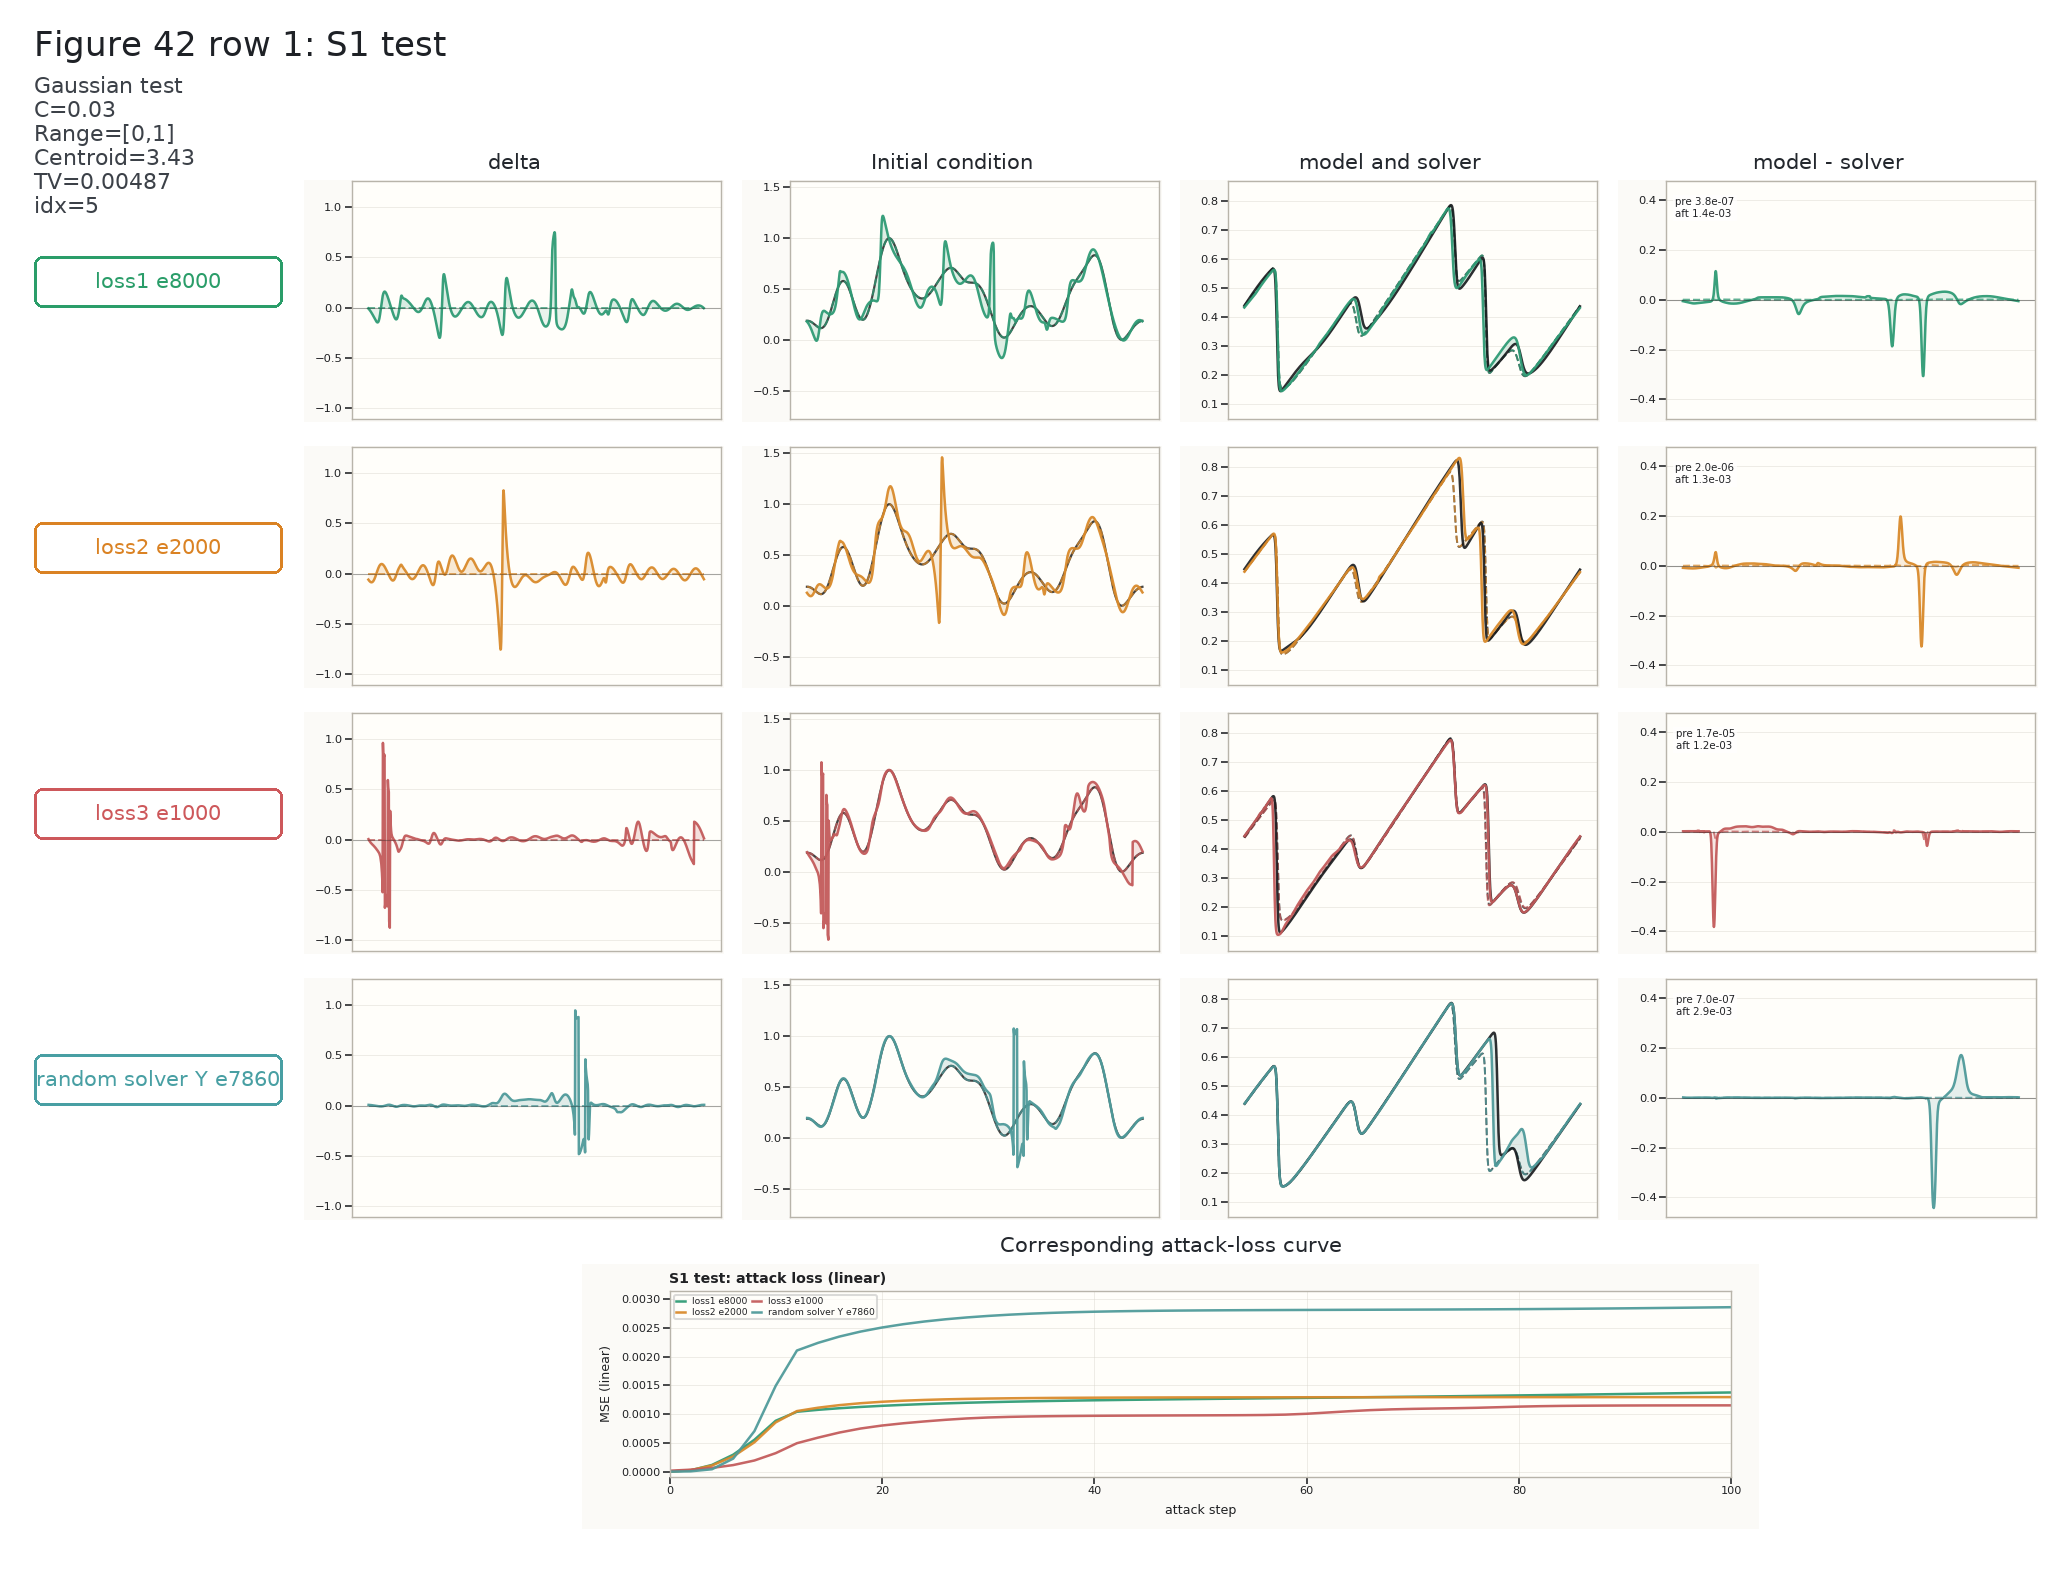
\includegraphics[width=0.99\textwidth,height=0.82\textheight,keepaspectratio]{figures/adversarial_attack_appendix/training/burgers/training_diagnostics/slide53_burgers_training_delta_sample_grid_rearranged_row1.png}
  \caption{Burgers post-training perturbation sample grid comparing the models obtained
  from Loss 1, Loss 2, Loss 3, and random-solver adversarial training, shown as
  route 1 of 6. Baseline and random clean are not plotted; the displayed models
  are evaluated on the same selected initial conditions. After training, all
  models are attacked with the same Loss 3 adversarial attack, so the labels
  denote the training objective rather than different evaluation objectives.}
  \label{fig:app-g-burgers-training-delta-grid}
\end{figure}

\clearpage
\begin{figure}[H]\ContinuedFloat
  \centering
  \captionsetup{skip=1pt}
  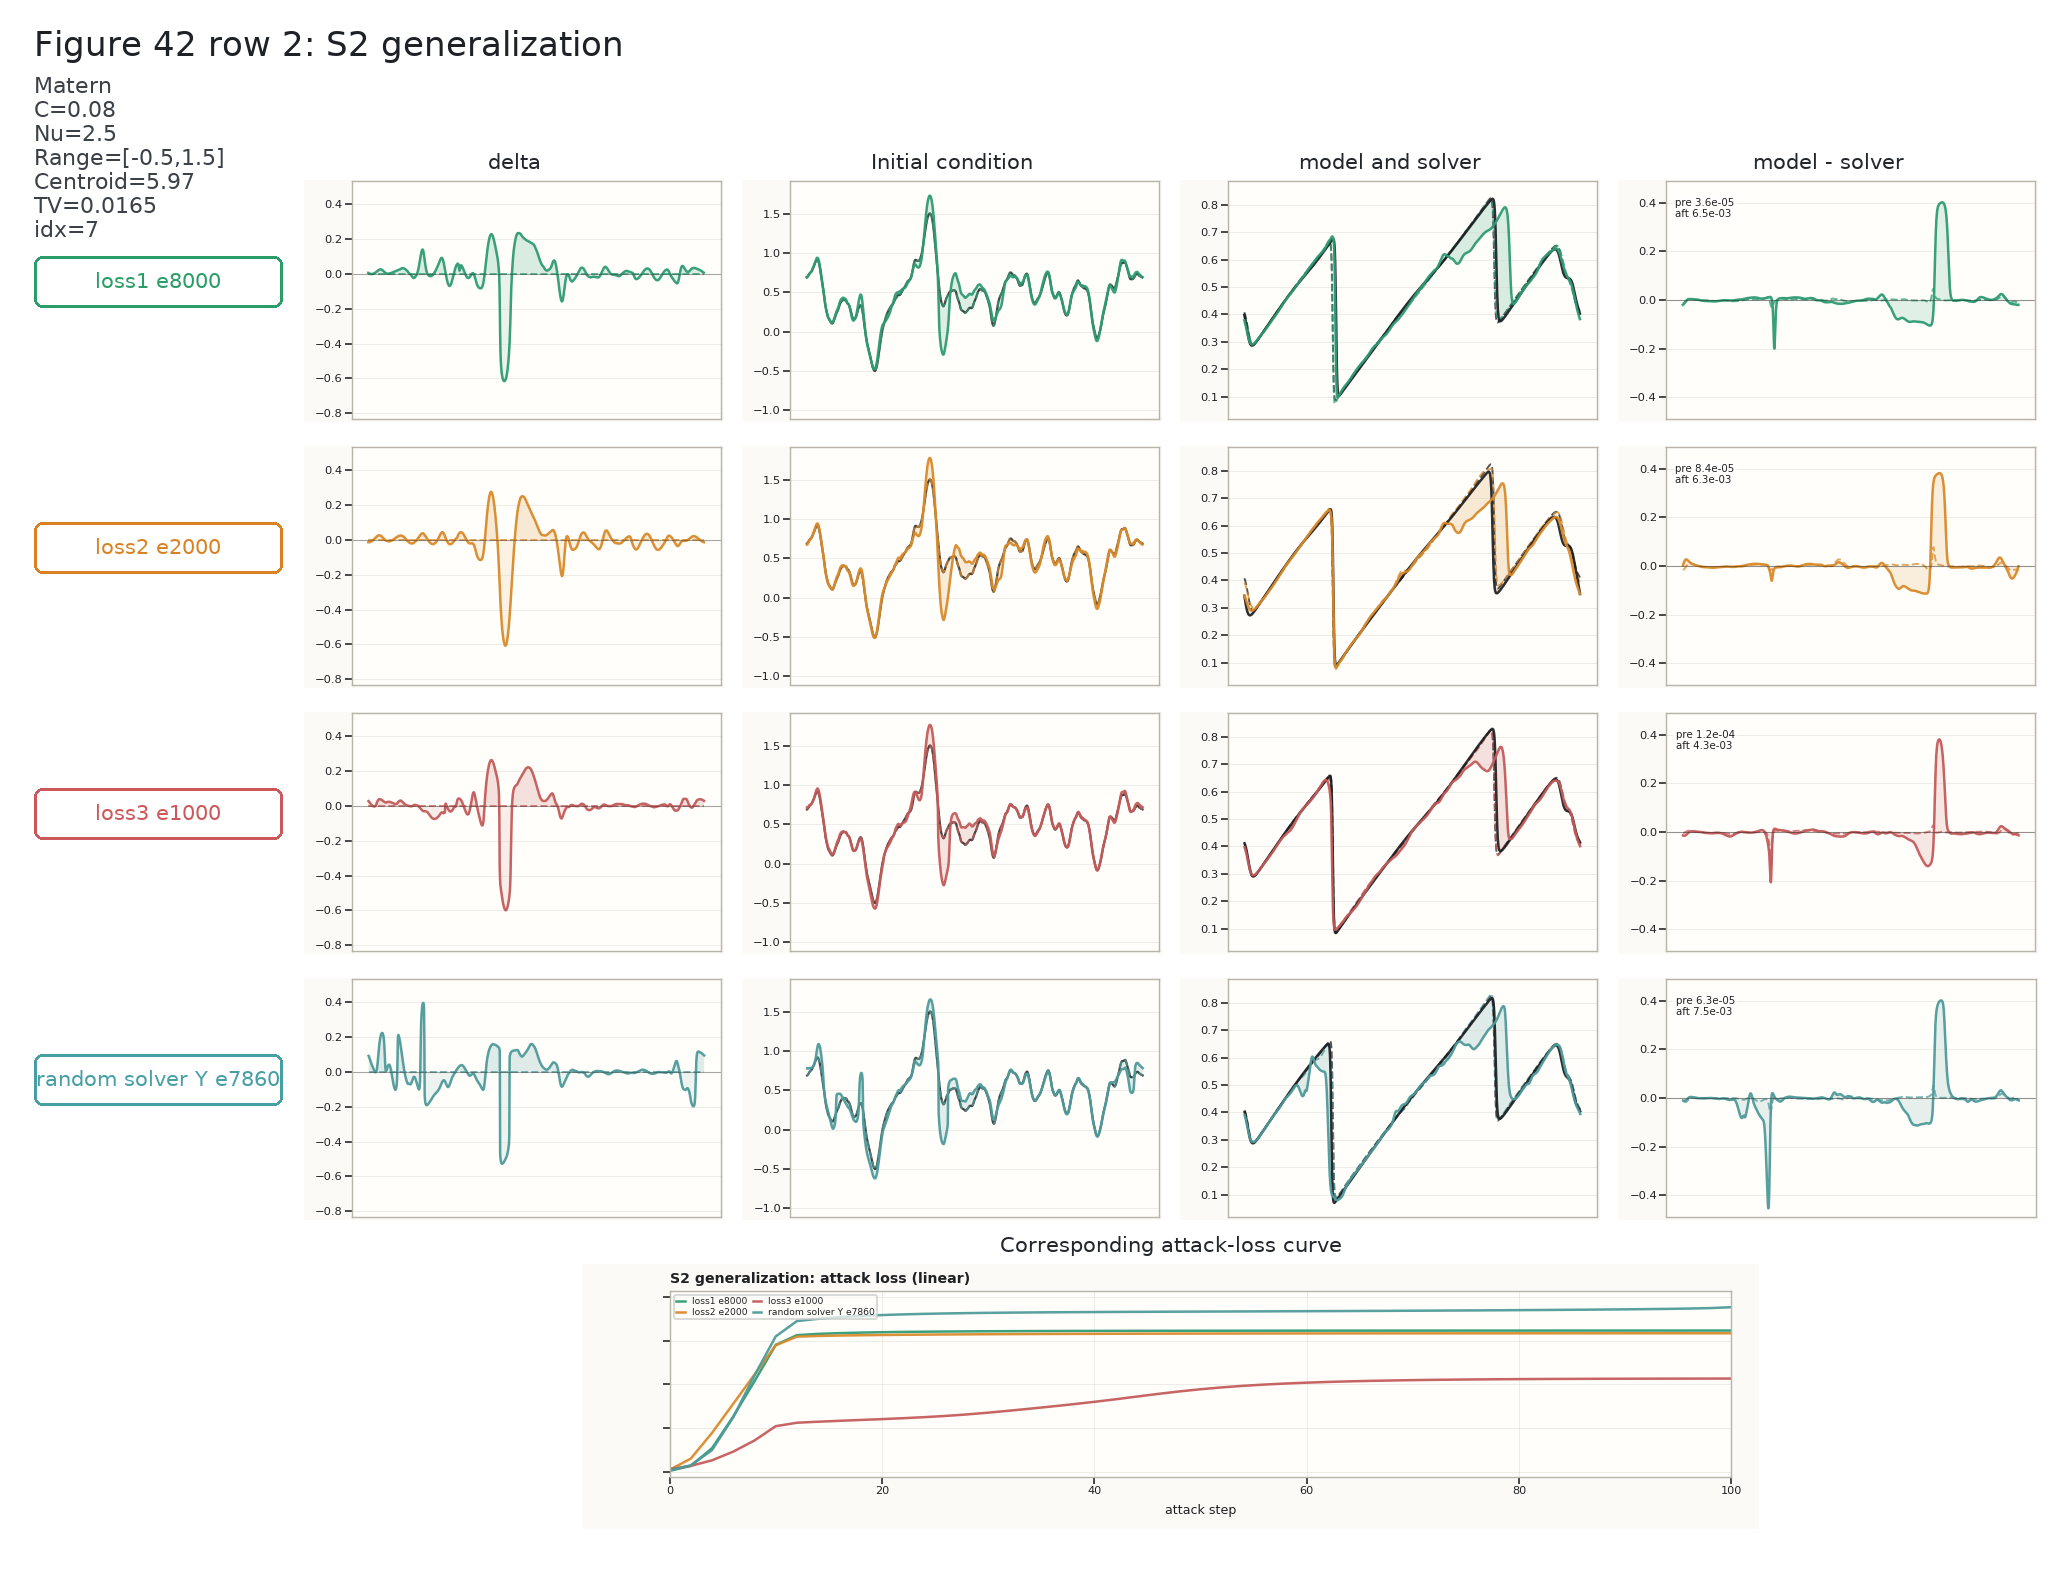
\includegraphics[width=0.99\textwidth,height=0.82\textheight,keepaspectratio]{figures/adversarial_attack_appendix/training/burgers/training_diagnostics/slide53_burgers_training_delta_sample_grid_rearranged_row2.png}
  \caption{Burgers post-training perturbation sample grid, route 2 of 6.}
\end{figure}

\clearpage
\begin{figure}[H]\ContinuedFloat
  \centering
  \captionsetup{skip=1pt}
  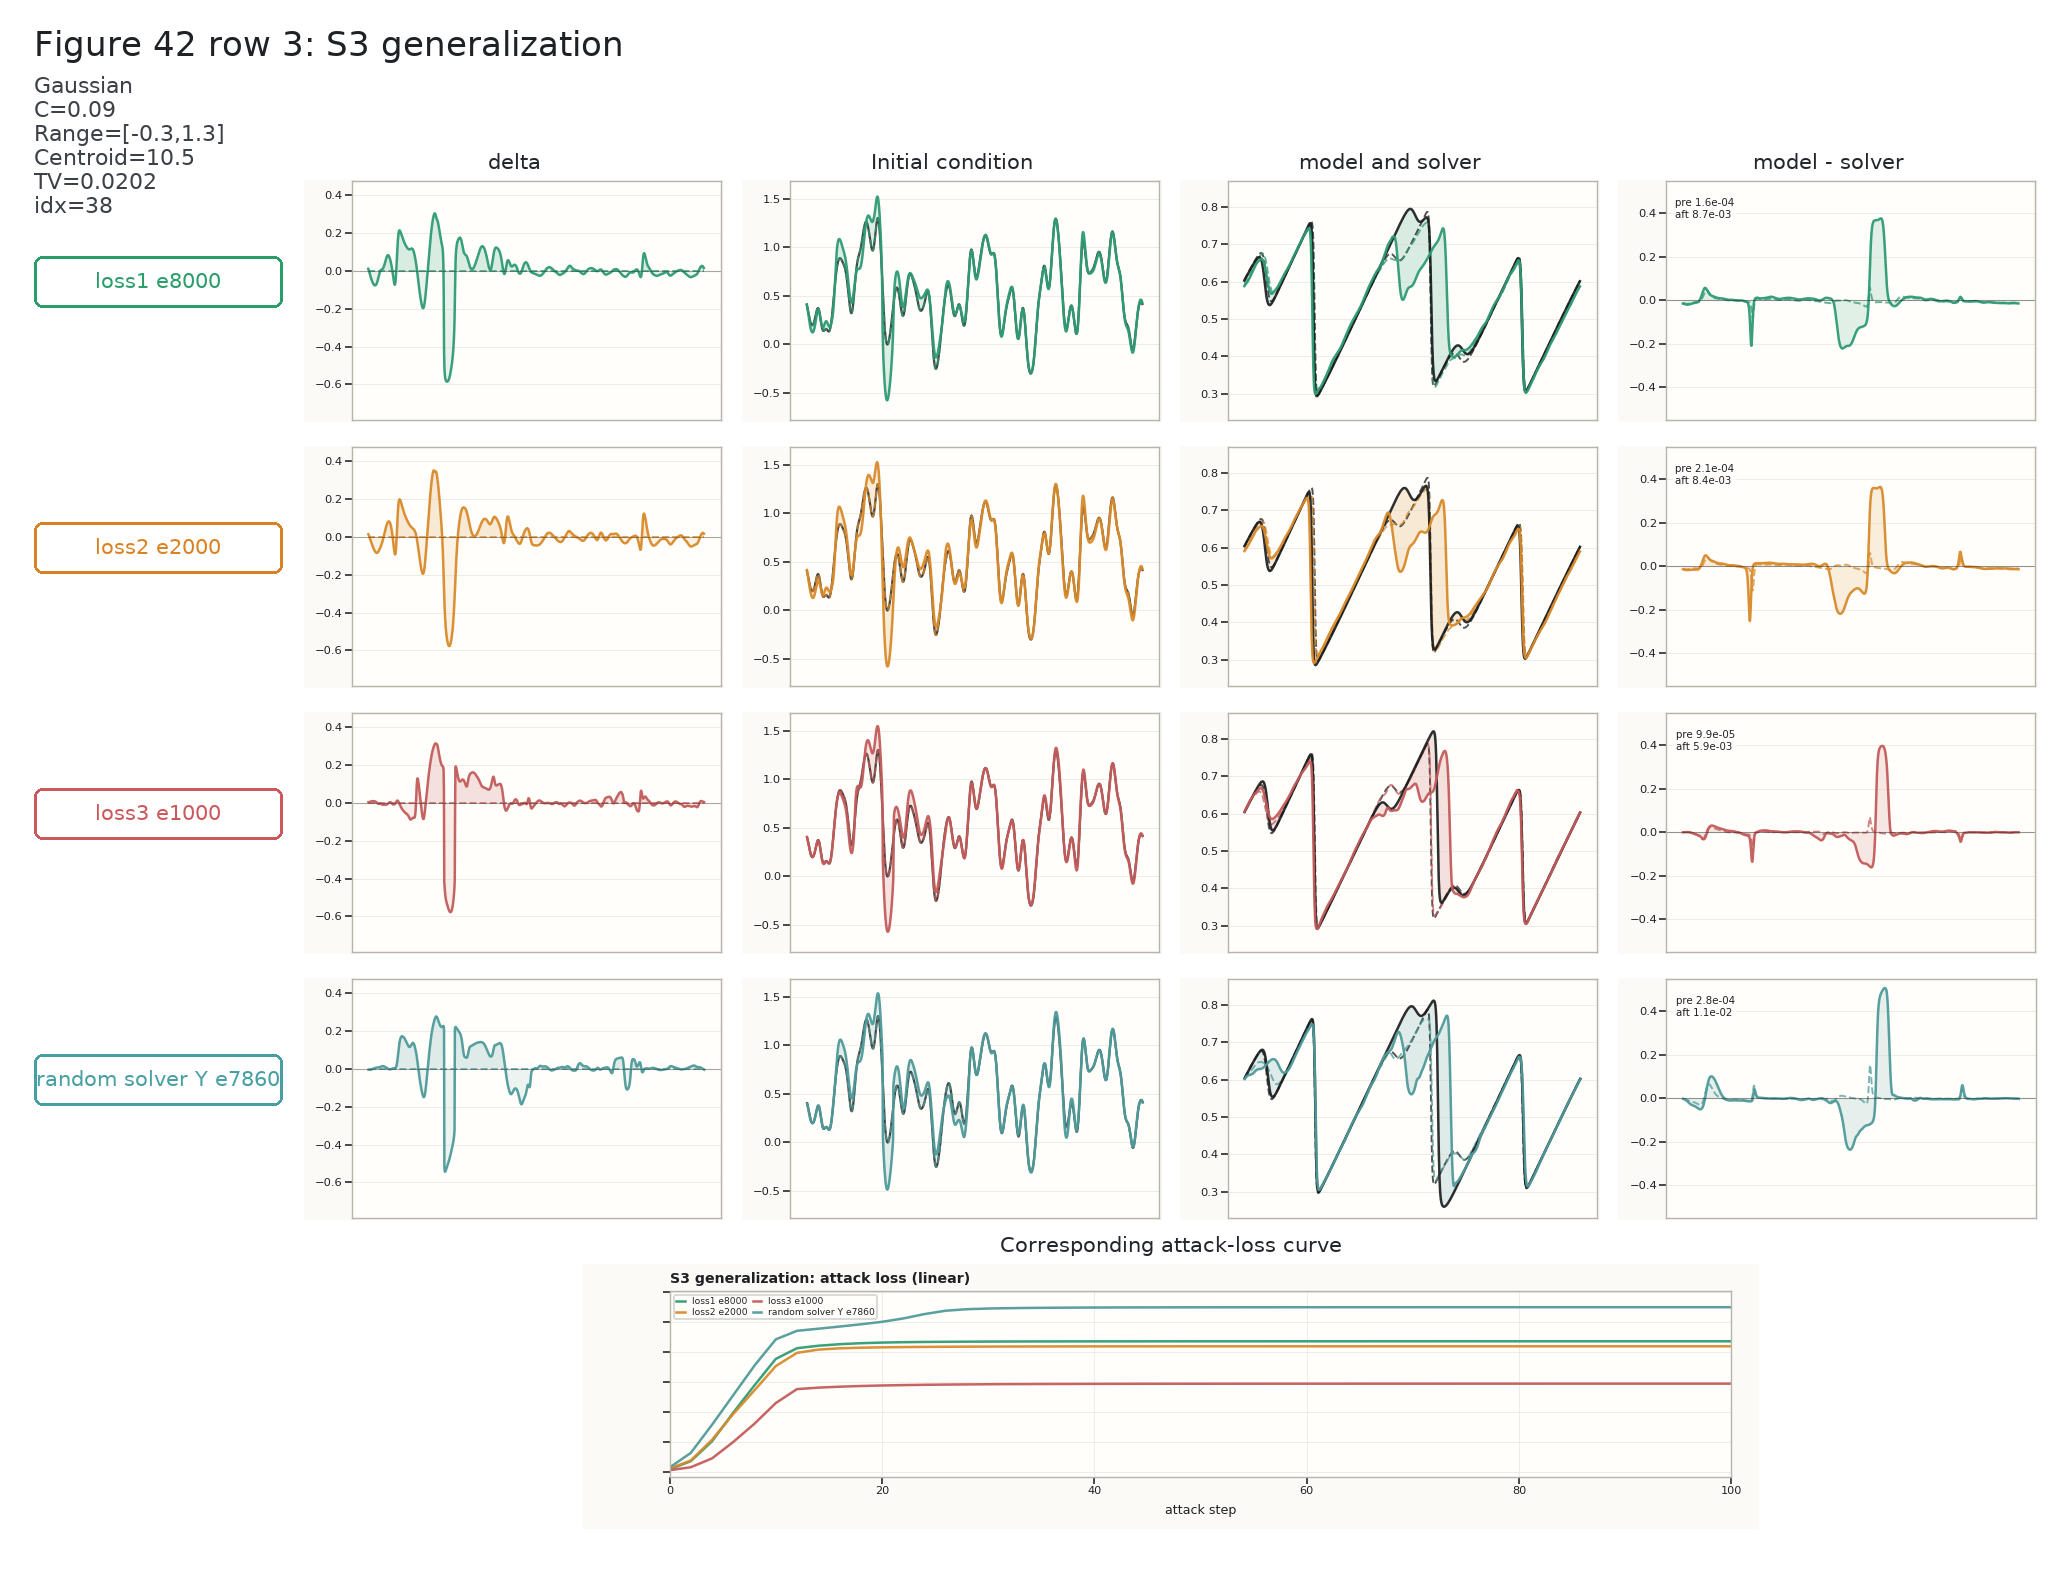
\includegraphics[width=0.99\textwidth,height=0.82\textheight,keepaspectratio]{figures/adversarial_attack_appendix/training/burgers/training_diagnostics/slide53_burgers_training_delta_sample_grid_rearranged_row3.png}
  \caption{Burgers post-training perturbation sample grid, route 3 of 6.}
\end{figure}

\clearpage
\begin{figure}[H]\ContinuedFloat
  \centering
  \captionsetup{skip=1pt}
  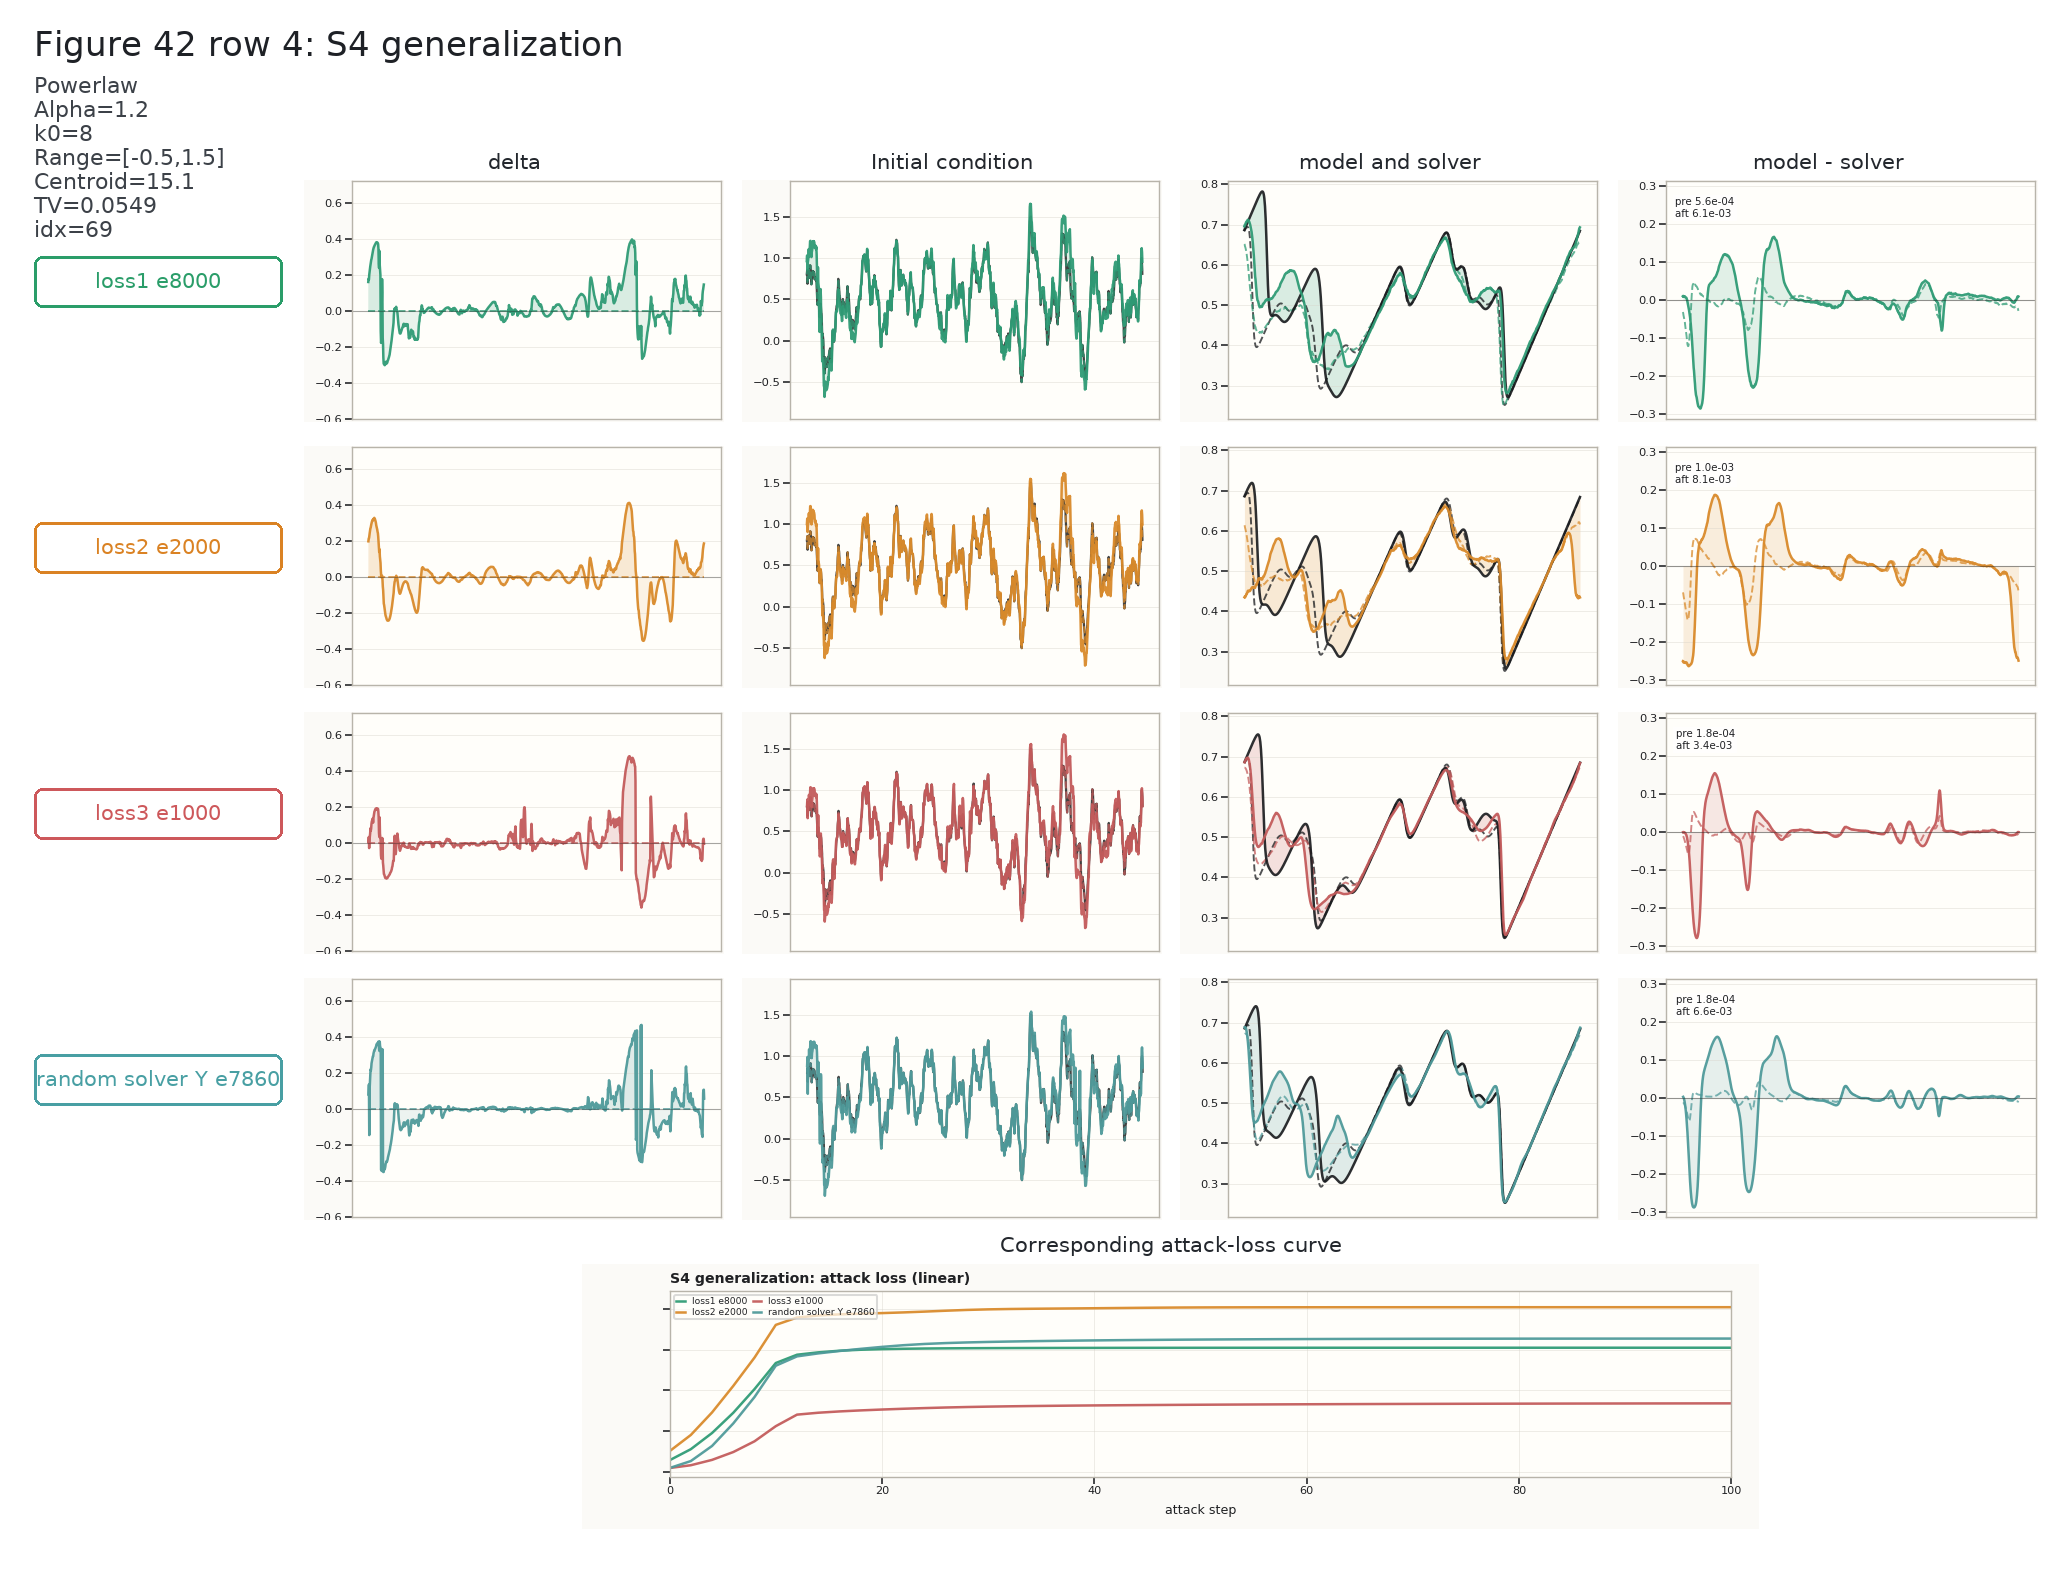
\includegraphics[width=0.99\textwidth,height=0.82\textheight,keepaspectratio]{figures/adversarial_attack_appendix/training/burgers/training_diagnostics/slide53_burgers_training_delta_sample_grid_rearranged_row4.png}
  \caption{Burgers post-training perturbation sample grid, route 4 of 6.}
\end{figure}

\clearpage
\begin{figure}[H]\ContinuedFloat
  \centering
  \captionsetup{skip=1pt}
  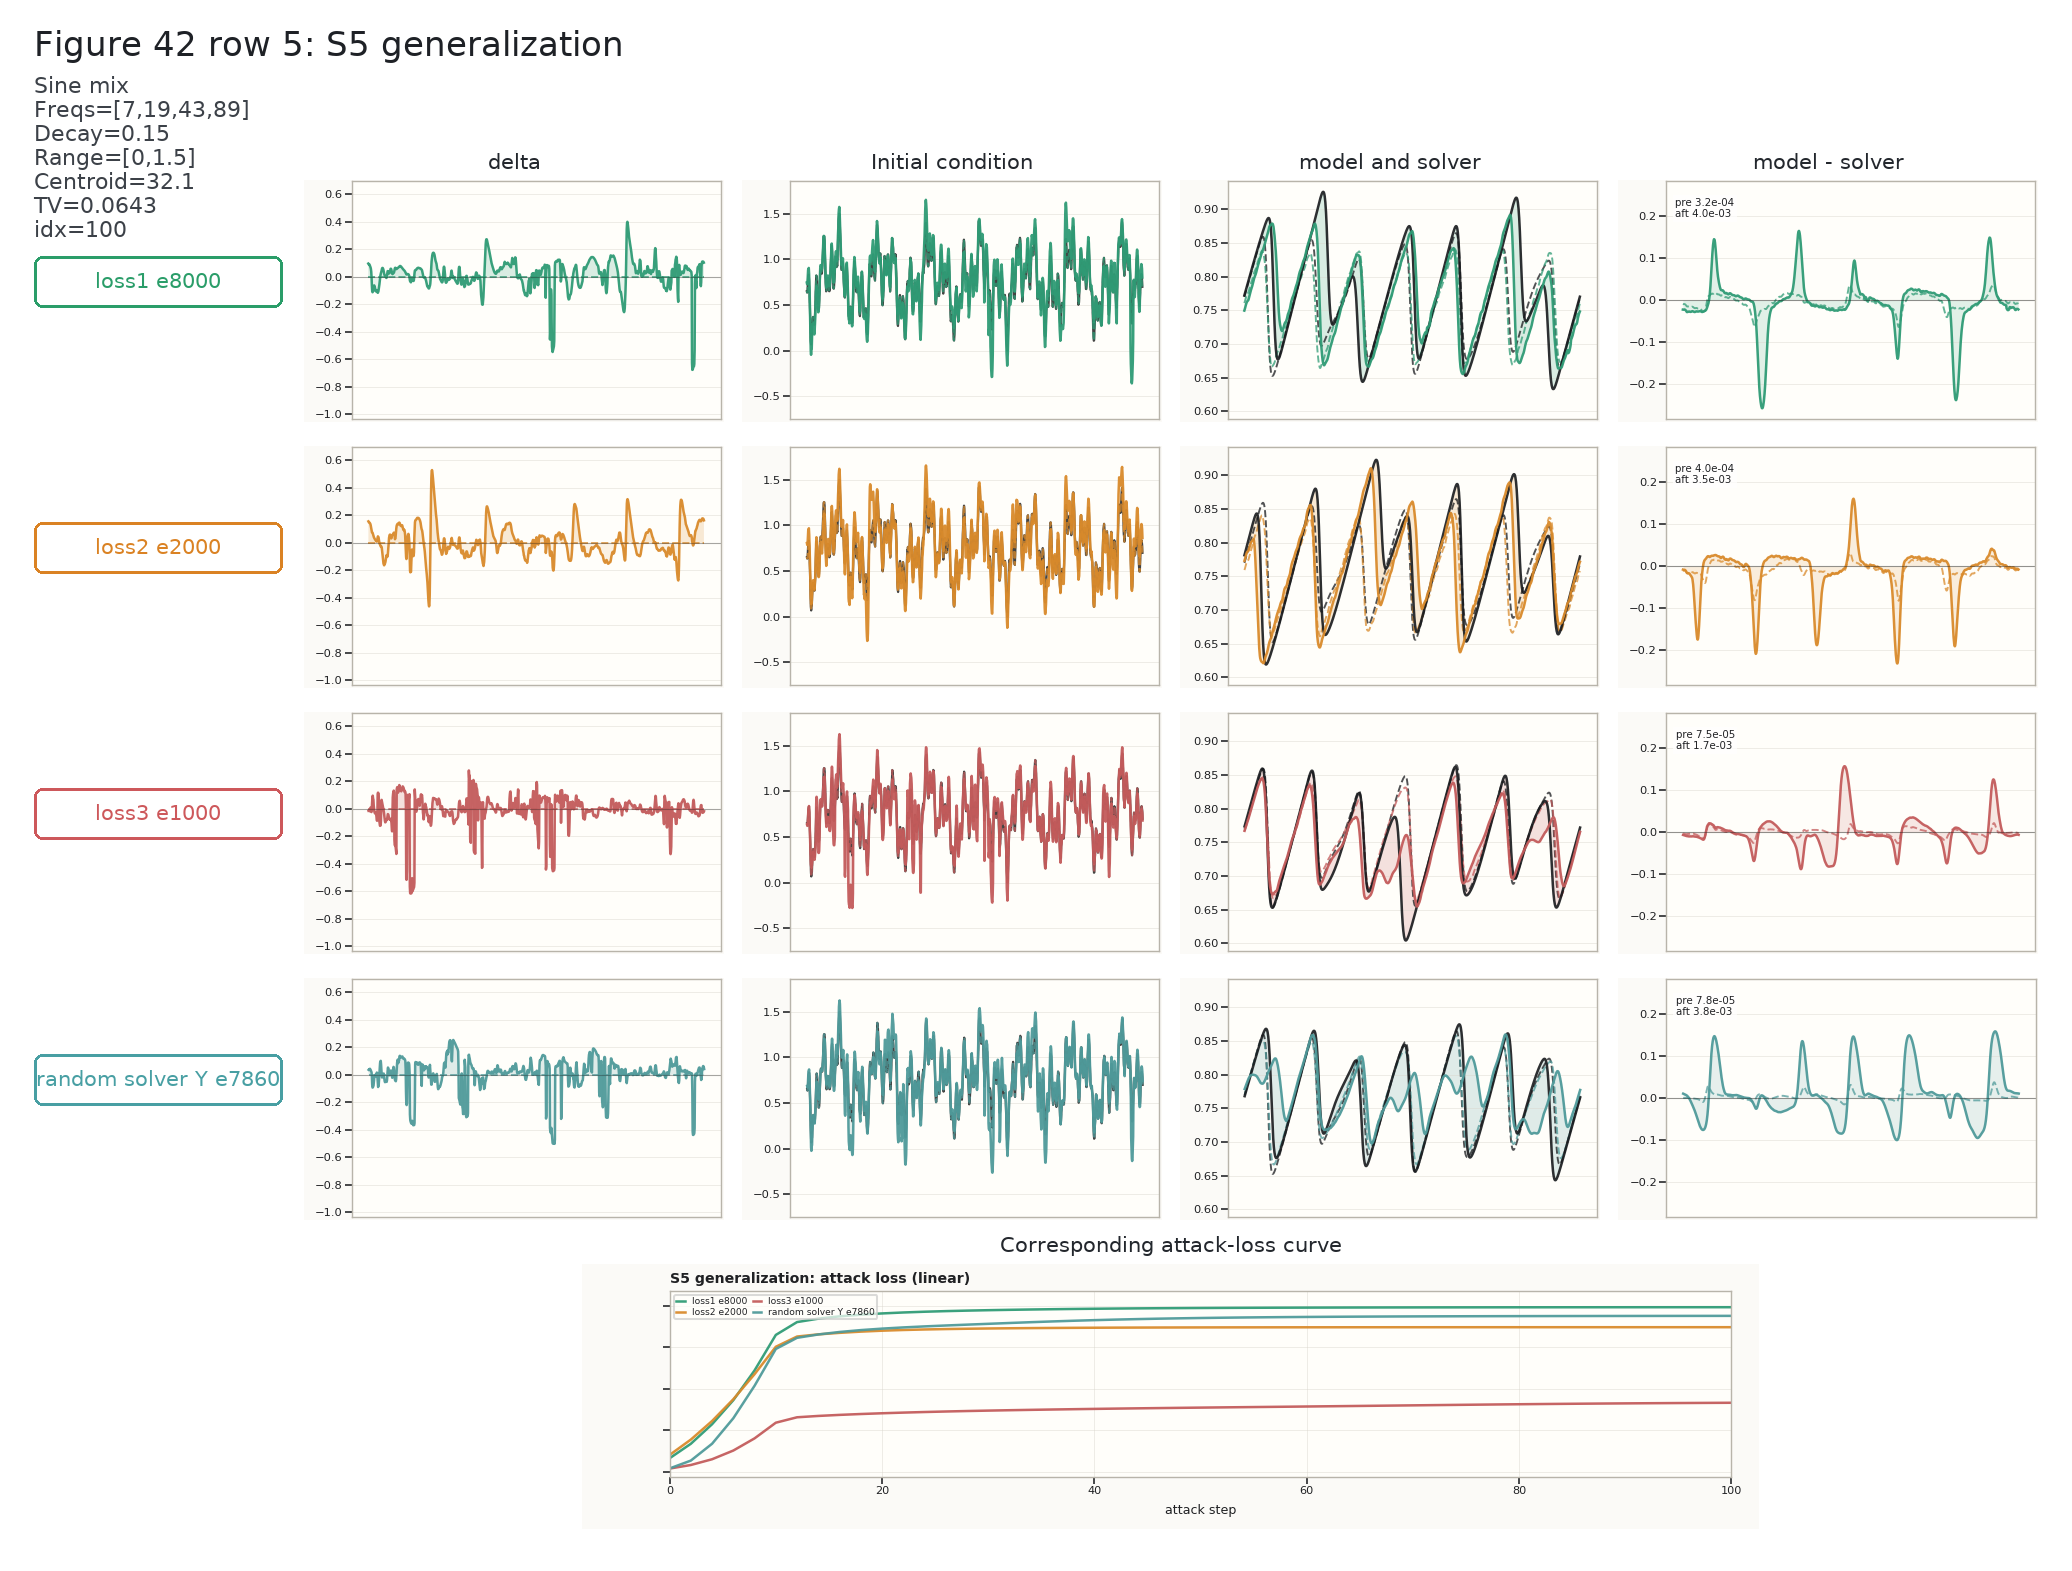
\includegraphics[width=0.99\textwidth,height=0.82\textheight,keepaspectratio]{figures/adversarial_attack_appendix/training/burgers/training_diagnostics/slide53_burgers_training_delta_sample_grid_rearranged_row5.png}
  \caption{Burgers post-training perturbation sample grid, route 5 of 6.}
\end{figure}

\clearpage
\begin{figure}[H]\ContinuedFloat
  \centering
  \captionsetup{skip=1pt}
  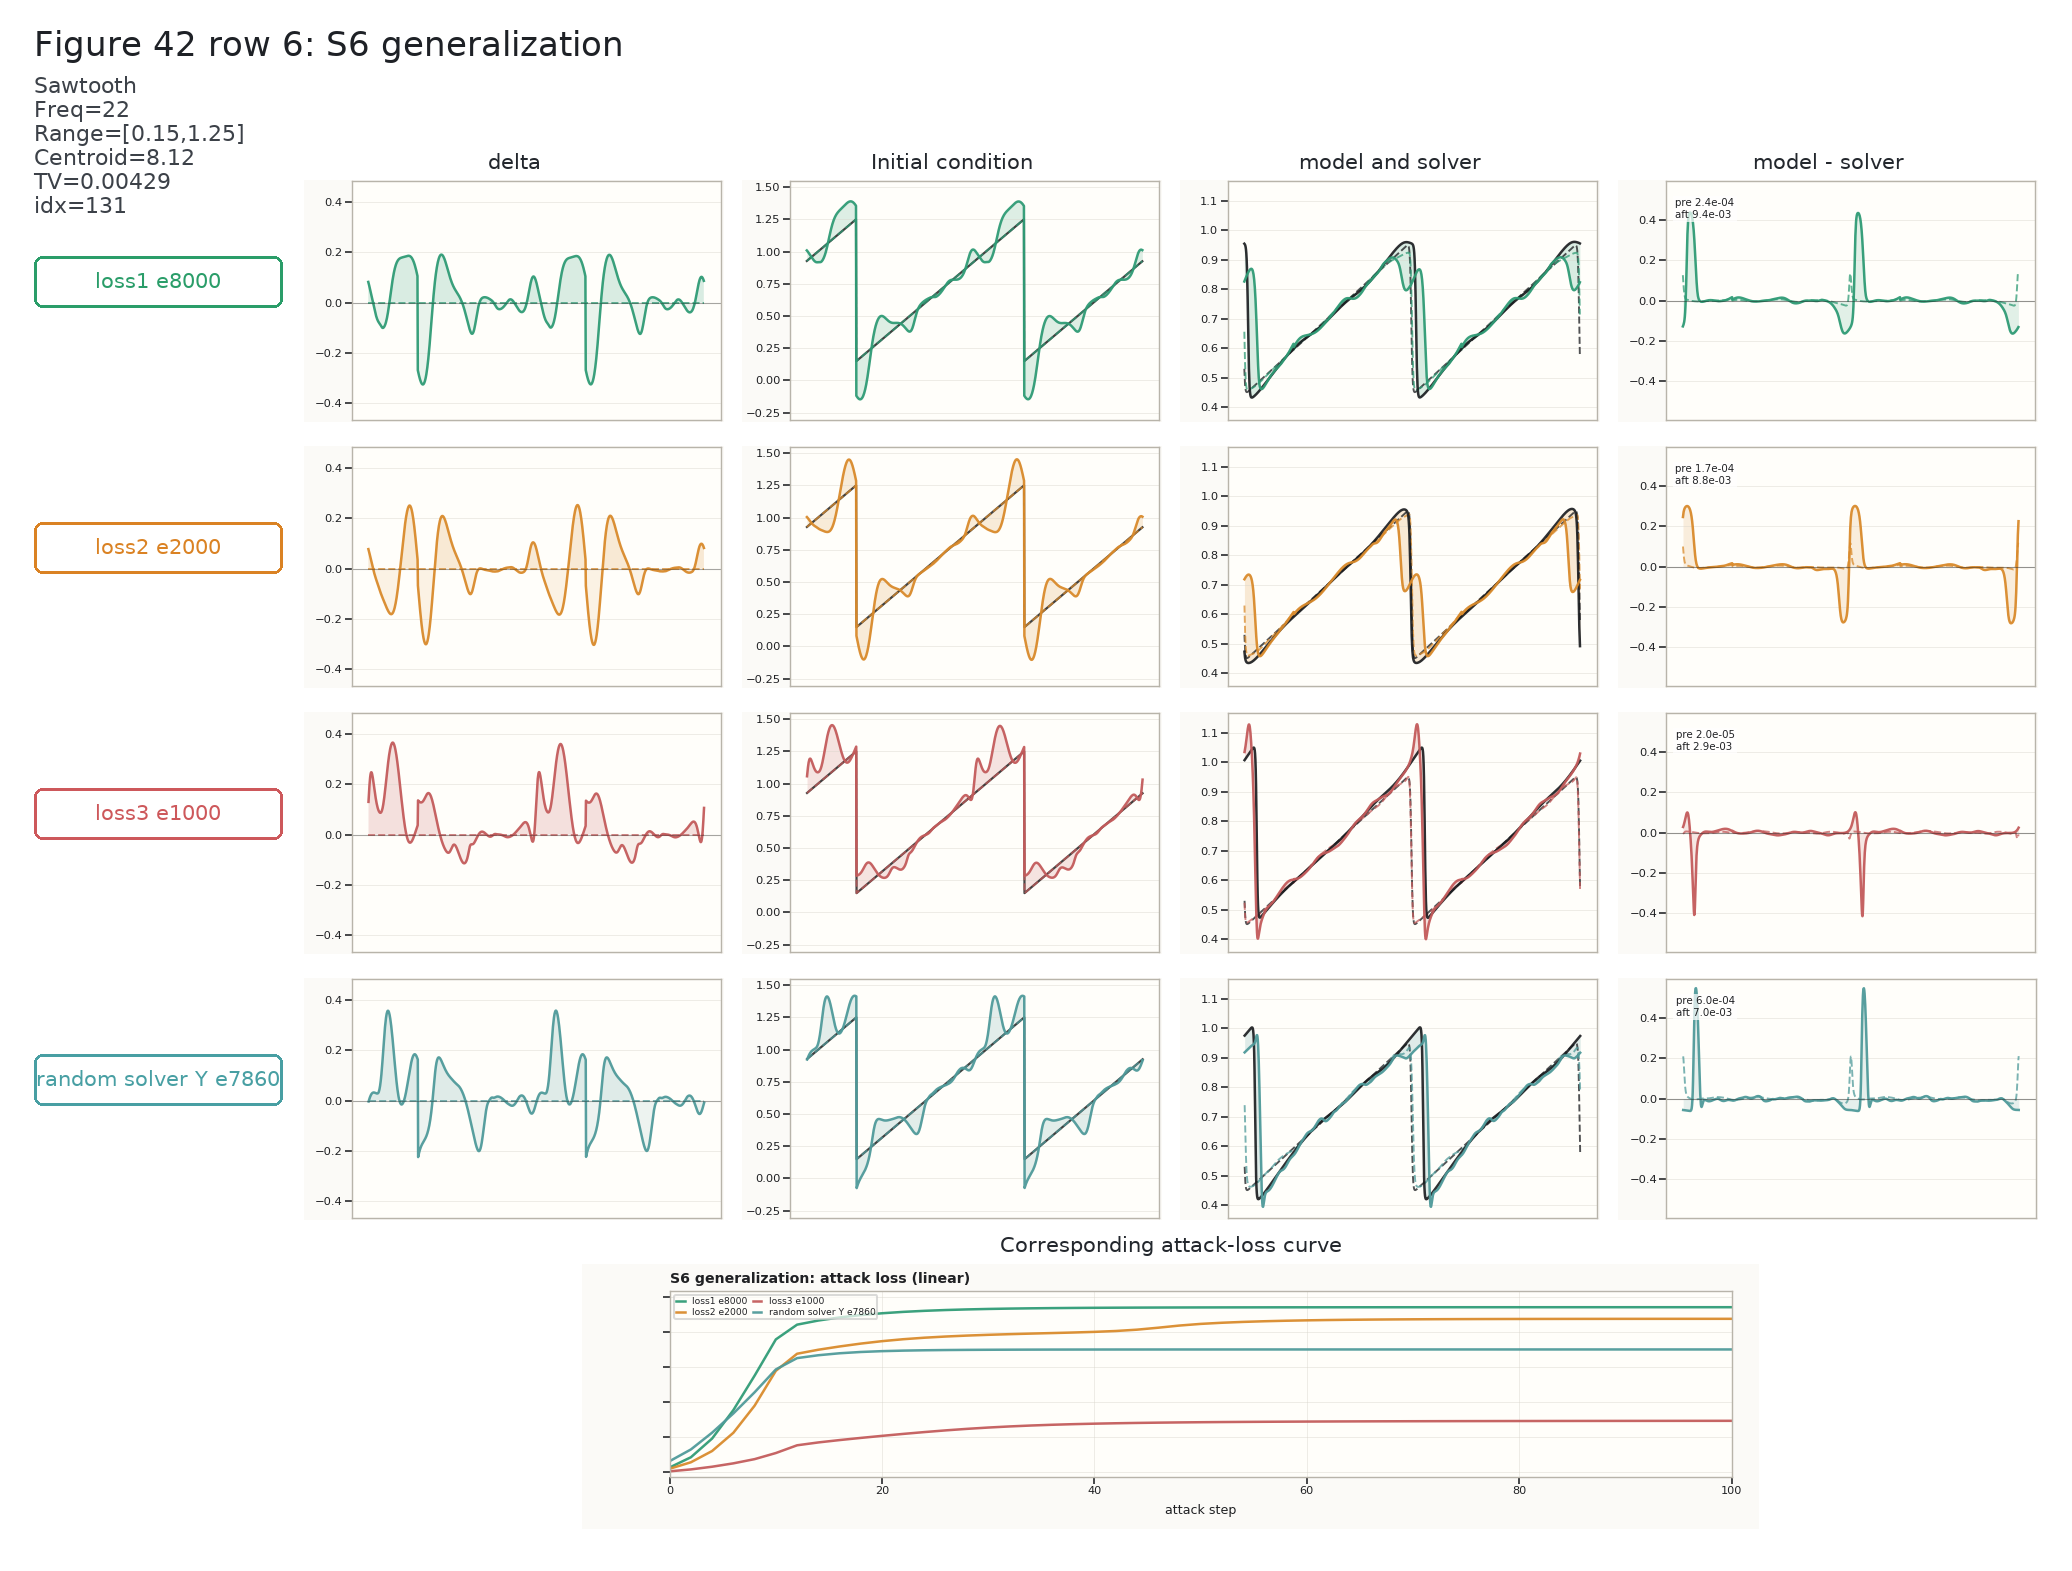
\includegraphics[width=0.99\textwidth,height=0.82\textheight,keepaspectratio]{figures/adversarial_attack_appendix/training/burgers/training_diagnostics/slide53_burgers_training_delta_sample_grid_rearranged_row6.png}
  \caption{Burgers post-training perturbation sample grid, route 6 of 6. The
  Loss 3-trained model has a smaller final loss increase, indicating the
  strongest robustness among these adversarial training variants.}
\end{figure}

\clearpage
\noindent\textbf{Epsilon attack sweep.}

\appendixattackfig
  {figures/adversarial_attack_appendix/training/burgers/epsilon_attack_sweeps/burgers_epsilon_vs_loss_increase_best_envelope_loglog.png}
  {Burgers adversarial-training epsilon attack sweep under the same adversarial
  attack budget, showing the absolute final attack loss increase over the
  initial loss on log-log axes. Among the trained methods, Burgers loss 3 has
  the smallest loss increase across attack budgets, showing that it is the most
  robust model under the matched adversarial attack objective.}
  {fig:app-g-burgers-training-epsilon-loss-increase}

\clearpage
\appendixdomainheading{Darcy Flow}

\noindent\textbf{Training diagnostics and perturbation samples.}

\appendixattackfig
  {figures/adversarial_attack_appendix/training/darcy_flow/training_diagnostics/slide57_darcy_flow_binary_loss3_attack_sample_grid.png}
  {Darcy Flow binary loss-3 training sample grid, including coefficient,
  perturbation, model, solver, residual, and loss-growth panels.}
  {fig:app-g-darcy-training-binary-loss3-sample-grid}

\noindent\textbf{Generalization curves.}

\appendixattackfigfullwidth
  {figures/adversarial_attack_appendix/training/darcy_flow/generalization_curves/slide54_darcy_flow_six_method_relative_l2_mean_curves.png}
  {Darcy Flow six-method relative $L_2$ train, test, and generalization mean
  curves. Loss 3 gives the strongest improvement on the generalization data. On
  the training and test splits, Loss 3 performs worse than the other methods.}
  {fig:app-g-darcy-training-mean-curves}

\clearpage

\appendixattackfigfullwidth
  {figures/adversarial_attack_appendix/training/darcy_flow/generalization_curves/slide55_darcy_flow_generalization_relative_l2_datasets_01_25.png}
  {Darcy Flow generalization relative $L_2$ curves for datasets 1--25. Across
  these held-out cases, Loss 3 generally reaches lower generalization loss and
  decreases faster than the competing training strategies.}
  {fig:app-g-darcy-training-gen-1-25}

\clearpage

\appendixattackfigfullwidth
  {figures/adversarial_attack_appendix/training/darcy_flow/generalization_curves/slide56_darcy_flow_generalization_relative_l2_datasets_26_50.png}
  {Darcy Flow generalization relative $L_2$ curves for datasets 26--50. These
  panels show the same pattern: the Loss 3 training objective tends to improve
  generalization more consistently and often reduces loss more quickly.}
  {fig:app-g-darcy-training-gen-26-50}

\clearpage
\noindent\textbf{Epsilon attack sweep.}

\appendixattackfig
  {figures/adversarial_attack_appendix/training/darcy_flow/epsilon_attack_sweeps/darcy_flow_epsilon_vs_loss_increase_best_envelope_loglog.png}
  {Darcy Flow adversarial-training epsilon attack sweep under the same attack
  budget. After training, the Loss 3 model has the smallest loss increase under
  the matched adversarial attack, indicating that it is the most robust among
  the compared Darcy Flow models.}
  {fig:app-g-darcy-training-epsilon-loss-increase}

\FloatBarrier
\appendixdomainheading{Navier--Stokes}

\appendixattackfig
  {figures/adversarial_attack_appendix/training/navier_stokes/generalization/slide59_ns2d_fno2d_generalizability_delta_rmse_bar_chart.png}
  {Navier--Stokes/FNO2d generalizability $\Delta$RMSE bar chart. Because
  Navier--Stokes adversarial training requires very large GPU memory and
  wall-clock time, we did not have enough compute for a complete systematic
  comparison. Instead, we ran six rounds of Loss 3 adversarial training on the
  FNO2d dataset and evaluated the trained model against the baseline on broad
  generalization datasets. Most cases show lower MSE after training, while a few
  increase, supporting the effectiveness of the method while also showing its
  practical limitation on memory- and time-intensive problems.}
  {fig:app-g-ns-training-delta-rmse}

\endgroup

\FloatBarrier

